\subsubsection{Two-dimensional case}
We are interested in estimating the exit time of a particle from a domain $D\subset\mathbb{R}^2$. Given $W(t)$ a  vector of two independent Brownian motions, we consider the equation \eqref{eq:GeneralModel}. In this case, $f\colon \mathbb{R}^2 \rightarrow \mathbb{R}^2, g\colon \mathbb{R}^2 \rightarrow \mathbb{R}^{2\times 2}$. We compute the mean exit time and the exit probability using DEM and CEM and compare results with the numerical solution of the PDE's presented in \ref{sec:PDEs}.


\vspace{2mm}
\noindent \textbf{Estimation of the exit time.} We consider a simple case of \eqref{eq:GeneralModel} in $D = [-1,1]^2$, where
\begin{equation*}
	f = 0 \in \R^2, \; g = \sigma I\in \R^{2\times 2}, \sigma \in \mathbb{R}.
\end{equation*}
Moreover, we consider $\partial D$ to be a killing boundary. The solution in this case is a Brownian motion. In this case, the partial differential equation \eqref{eq:PDETau} reduces to
\begin{equation}\label{eq:PDETau2DKilling}
	\left \{
  	\begin{aligned}
	- \sigma^2 \Delta \bar \tau &= 2, && \text{in } D, \\
	\bar \tau &= 0, && \text{on } \partial D.
	\end{aligned} \right.
\end{equation}
This is the Poisson equation, hence it is possible to solve it numerically with the Finite Elements Method or the finite differences avoiding a high computational cost. We use the Finite Elements Method adopting a regular mesh with equal constant spacing in the $x$ and $y$ directions, obtaining a solution as in Figure \ref{fig:TauExact2DKill}. In order to verify the orders of convergence of DEM and CEM, we set $T = 3$, $\sigma = 1$, $X_0 = (0,0)^T$, with $M = 10^4$ and $N = 2^i,i=3,\dots,9$. We then compare the Montecarlo estimation with the value of $\bar\tau$ in $(0,0)$, obtained by an evaluation of the Finite Elements solution. The orders of convergence for this numerical experiment are shown in Figure \ref{fig:KillTwoD}. The results confirm the theoretical orders of convergence for DEM and CEM, with an average order of 0.55 for DEM and 0.93 for CEM, which corrects to 0.98 if the last point is not taken into account.

\begin{figure}[t]
    \centering
    \begin{subfigure}{0.49\linewidth}
        \centering
        \resizebox{1\linewidth}{!}{% This file was created by matlab2tikz.
%
%The latest updates can be retrieved from
%  http://www.mathworks.com/matlabcentral/fileexchange/22022-matlab2tikz-matlab2tikz
%where you can also make suggestions and rate matlab2tikz.
%
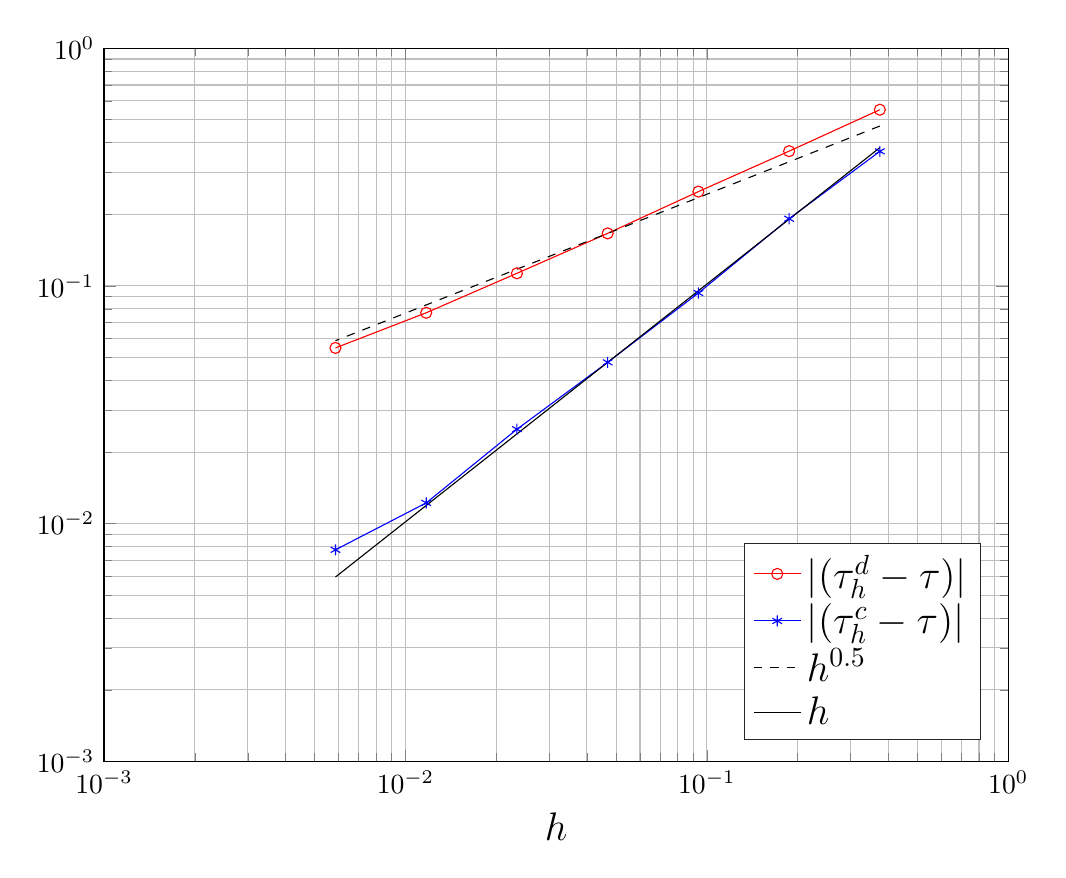
\begin{tikzpicture}

\begin{axis}[%
width=4.521in,
height=3.566in,
at={(0.758in,0.481in)},
scale only axis,
xmode=log,
xmin=0.001,
xmax=1,
xminorticks=true,
xlabel={$h$},
xlabel style={font=\Large},
xmajorgrids,
xminorgrids,
ymode=log,
ymin=0.001,
ymax=1,
yminorticks=true,
ymajorgrids,
yminorgrids,
axis background/.style={fill=white},
legend pos = south east,
legend style={legend cell align=left,align=left,draw=white!15!black,font=\Large}
]
\addplot [color=red,solid,mark=o,mark options={solid}]
  table[row sep=crcr]{%
0.375	0.550863107686105\\
0.1875	0.368781857686105\\
0.09375	0.249241232686105\\
0.046875	0.166314670186105\\
0.0234375	0.112973263936105\\
0.01171875	0.077078732686105\\
0.005859375	0.054845920186105\\
};
\addlegendentry{$|\E(\tau_h^d - \tau)|$};

\addplot [color=blue,solid,mark=asterisk,mark options={solid}]
  table[row sep=crcr]{%
0.375	0.368013107686105\\
0.1875	0.191688107686105\\
0.09375	0.0933443576861051\\
0.046875	0.047697482686105\\
0.0234375	0.024953732686105\\
0.01171875	0.012223654561105\\
0.005859375	0.00776291237360505\\
};
\addlegendentry{$|\E(\tau_h^c - \tau)|$};

\addplot [color=black,dashed]
  table[row sep=crcr]{%
0.375	0.470408924397596\\
0.1875	0.33262934037221\\
0.09375	0.235204462198798\\
0.046875	0.166314670186105\\
0.0234375	0.117602231099399\\
0.01171875	0.0831573350930525\\
0.005859375	0.0588011155496995\\
};
\addlegendentry{$h^{0.5}$};

\addplot [color=black,solid]
  table[row sep=crcr]{%
0.375	0.38157986148884\\
0.1875	0.19078993074442\\
0.09375	0.0953949653722099\\
0.046875	0.047697482686105\\
0.0234375	0.0238487413430525\\
0.01171875	0.0119243706715262\\
0.005859375	0.00596218533576312\\
};
\addlegendentry{$h$};

\end{axis}
\end{tikzpicture}%
 }  
        \caption{Convergence of CEM and DEM.}
        \label{fig:KillTwoD}
    \end{subfigure}
    \begin{subfigure}{0.49\linewidth}
        \centering
        \resizebox{1\linewidth}{!}{% This file was created by matlab2tikz.
%
%The latest updates can be retrieved from
%  http://www.mathworks.com/matlabcentral/fileexchange/22022-matlab2tikz-matlab2tikz
%where you can also make suggestions and rate matlab2tikz.
%
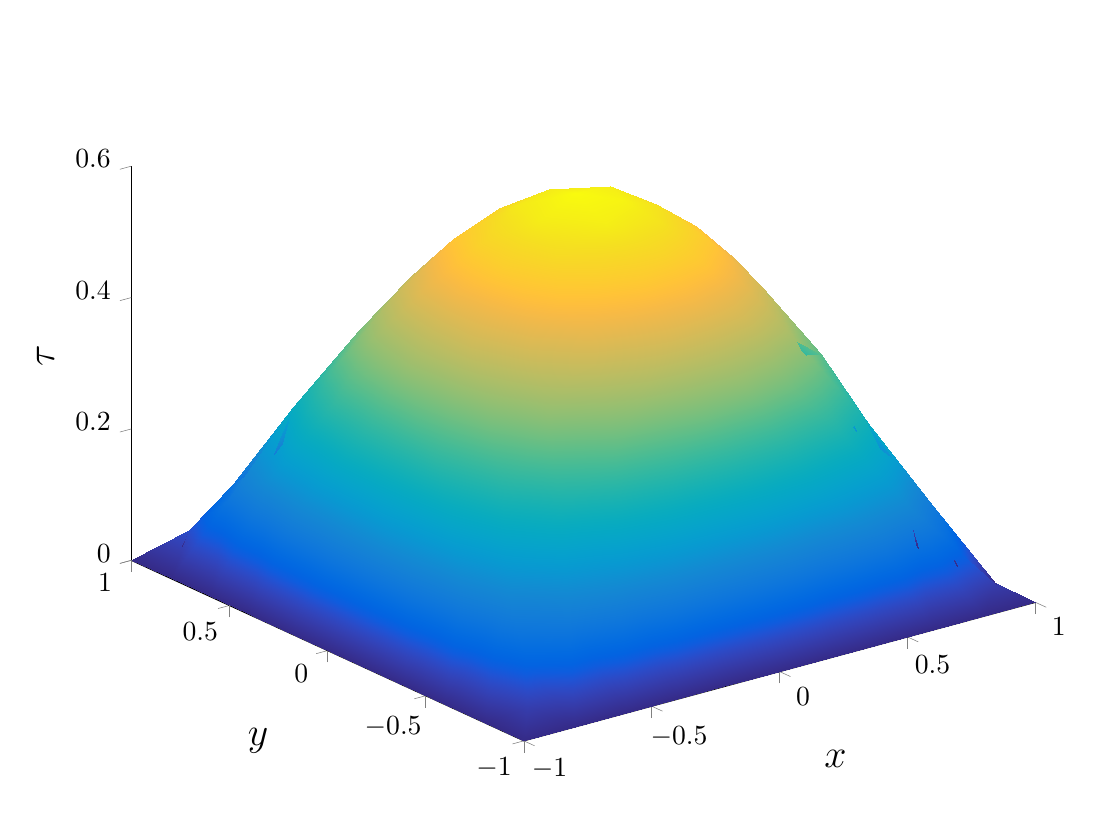
\begin{tikzpicture}

\begin{axis}[%
width=4.521in,
height=3.566in,
at={(0.758in,0.481in)},
scale only axis,
colormap={mymap}{[1pt] rgb(0pt)=(0.2081,0.1663,0.5292); rgb(1pt)=(0.211624,0.189781,0.577676); rgb(2pt)=(0.212252,0.213771,0.626971); rgb(3pt)=(0.2081,0.2386,0.677086); rgb(4pt)=(0.195905,0.264457,0.7279); rgb(5pt)=(0.170729,0.291938,0.779248); rgb(6pt)=(0.125271,0.324243,0.830271); rgb(7pt)=(0.0591333,0.359833,0.868333); rgb(8pt)=(0.0116952,0.38751,0.881957); rgb(9pt)=(0.00595714,0.408614,0.882843); rgb(10pt)=(0.0165143,0.4266,0.878633); rgb(11pt)=(0.0328524,0.443043,0.871957); rgb(12pt)=(0.0498143,0.458571,0.864057); rgb(13pt)=(0.0629333,0.47369,0.855438); rgb(14pt)=(0.0722667,0.488667,0.8467); rgb(15pt)=(0.0779429,0.503986,0.838371); rgb(16pt)=(0.0793476,0.520024,0.831181); rgb(17pt)=(0.0749429,0.537543,0.826271); rgb(18pt)=(0.0640571,0.556986,0.823957); rgb(19pt)=(0.0487714,0.577224,0.822829); rgb(20pt)=(0.0343429,0.596581,0.819852); rgb(21pt)=(0.0265,0.6137,0.8135); rgb(22pt)=(0.0238905,0.628662,0.803762); rgb(23pt)=(0.0230905,0.641786,0.791267); rgb(24pt)=(0.0227714,0.653486,0.776757); rgb(25pt)=(0.0266619,0.664195,0.760719); rgb(26pt)=(0.0383714,0.674271,0.743552); rgb(27pt)=(0.0589714,0.683757,0.725386); rgb(28pt)=(0.0843,0.692833,0.706167); rgb(29pt)=(0.113295,0.7015,0.685857); rgb(30pt)=(0.145271,0.709757,0.664629); rgb(31pt)=(0.180133,0.717657,0.642433); rgb(32pt)=(0.217829,0.725043,0.619262); rgb(33pt)=(0.258643,0.731714,0.595429); rgb(34pt)=(0.302171,0.737605,0.571186); rgb(35pt)=(0.348167,0.742433,0.547267); rgb(36pt)=(0.395257,0.7459,0.524443); rgb(37pt)=(0.44201,0.748081,0.503314); rgb(38pt)=(0.487124,0.749062,0.483976); rgb(39pt)=(0.530029,0.749114,0.466114); rgb(40pt)=(0.570857,0.748519,0.44939); rgb(41pt)=(0.609852,0.747314,0.433686); rgb(42pt)=(0.6473,0.7456,0.4188); rgb(43pt)=(0.683419,0.743476,0.404433); rgb(44pt)=(0.71841,0.741133,0.390476); rgb(45pt)=(0.752486,0.7384,0.376814); rgb(46pt)=(0.785843,0.735567,0.363271); rgb(47pt)=(0.818505,0.732733,0.34979); rgb(48pt)=(0.850657,0.7299,0.336029); rgb(49pt)=(0.882433,0.727433,0.3217); rgb(50pt)=(0.913933,0.725786,0.306276); rgb(51pt)=(0.944957,0.726114,0.288643); rgb(52pt)=(0.973895,0.731395,0.266648); rgb(53pt)=(0.993771,0.745457,0.240348); rgb(54pt)=(0.999043,0.765314,0.216414); rgb(55pt)=(0.995533,0.786057,0.196652); rgb(56pt)=(0.988,0.8066,0.179367); rgb(57pt)=(0.978857,0.827143,0.163314); rgb(58pt)=(0.9697,0.848138,0.147452); rgb(59pt)=(0.962586,0.870514,0.1309); rgb(60pt)=(0.958871,0.8949,0.113243); rgb(61pt)=(0.959824,0.921833,0.0948381); rgb(62pt)=(0.9661,0.951443,0.0755333); rgb(63pt)=(0.9763,0.9831,0.0538)},
xmin=-1,
xmax=1,
tick align=outside,
xlabel={$x$},
xlabel style={font=\Large},
ymin=-1,
ymax=1,
ylabel={$y$},
ylabel style={font=\Large},
zmin=0,
zmax=0.6,
zlabel={$\tau$},
zlabel style={font=\Large},
view={-37.5}{30},
axis background/.style={fill=white},
axis x line*=bottom,
axis y line*=left,
axis z line*=left
]

\addplot3[area legend,solid,table/row sep=crcr,patch,shader=interp,forget plot,patch table={%
0	1	2\\
3	4	5\\
6	7	8\\
9	10	11\\
12	13	14\\
15	16	17\\
18	19	20\\
21	22	23\\
24	25	26\\
27	28	29\\
30	31	32\\
33	34	35\\
36	37	38\\
39	40	41\\
42	43	44\\
45	46	47\\
48	49	50\\
51	52	53\\
54	55	56\\
57	58	59\\
60	61	62\\
63	64	65\\
66	67	68\\
69	70	71\\
72	73	74\\
75	76	77\\
78	79	80\\
81	82	83\\
84	85	86\\
87	88	89\\
90	91	92\\
93	94	95\\
96	97	98\\
99	100	101\\
102	103	104\\
105	106	107\\
108	109	110\\
111	112	113\\
114	115	116\\
117	118	119\\
120	121	122\\
123	124	125\\
126	127	128\\
129	130	131\\
132	133	134\\
135	136	137\\
138	139	140\\
141	142	143\\
144	145	146\\
147	148	149\\
150	151	152\\
153	154	155\\
156	157	158\\
159	160	161\\
162	163	164\\
165	166	167\\
168	169	170\\
171	172	173\\
174	175	176\\
177	178	179\\
180	181	182\\
183	184	185\\
186	187	188\\
189	190	191\\
192	193	194\\
195	196	197\\
198	199	200\\
201	202	203\\
204	205	206\\
207	208	209\\
210	211	212\\
213	214	215\\
216	217	218\\
219	220	221\\
222	223	224\\
225	226	227\\
228	229	230\\
231	232	233\\
234	235	236\\
237	238	239\\
240	241	242\\
243	244	245\\
246	247	248\\
249	250	251\\
252	253	254\\
255	256	257\\
258	259	260\\
261	262	263\\
264	265	266\\
267	268	269\\
270	271	272\\
273	274	275\\
276	277	278\\
279	280	281\\
282	283	284\\
285	286	287\\
288	289	290\\
291	292	293\\
294	295	296\\
297	298	299\\
300	301	302\\
303	304	305\\
306	307	308\\
309	310	311\\
312	313	314\\
315	316	317\\
318	319	320\\
321	322	323\\
324	325	326\\
327	328	329\\
330	331	332\\
333	334	335\\
336	337	338\\
339	340	341\\
342	343	344\\
345	346	347\\
348	349	350\\
351	352	353\\
354	355	356\\
357	358	359\\
360	361	362\\
363	364	365\\
366	367	368\\
369	370	371\\
372	373	374\\
375	376	377\\
378	379	380\\
381	382	383\\
384	385	386\\
387	388	389\\
390	391	392\\
393	394	395\\
396	397	398\\
399	400	401\\
402	403	404\\
405	406	407\\
408	409	410\\
411	412	413\\
414	415	416\\
417	418	419\\
420	421	422\\
423	424	425\\
426	427	428\\
429	430	431\\
432	433	434\\
435	436	437\\
438	439	440\\
441	442	443\\
444	445	446\\
447	448	449\\
450	451	452\\
453	454	455\\
456	457	458\\
459	460	461\\
462	463	464\\
465	466	467\\
468	469	470\\
471	472	473\\
474	475	476\\
477	478	479\\
480	481	482\\
483	484	485\\
486	487	488\\
489	490	491\\
492	493	494\\
495	496	497\\
498	499	500\\
501	502	503\\
504	505	506\\
507	508	509\\
510	511	512\\
513	514	515\\
516	517	518\\
519	520	521\\
522	523	524\\
525	526	527\\
528	529	530\\
531	532	533\\
534	535	536\\
537	538	539\\
540	541	542\\
543	544	545\\
546	547	548\\
549	550	551\\
552	553	554\\
555	556	557\\
558	559	560\\
561	562	563\\
564	565	566\\
567	568	569\\
570	571	572\\
573	574	575\\
576	577	578\\
579	580	581\\
582	583	584\\
585	586	587\\
588	589	590\\
591	592	593\\
594	595	596\\
597	598	599\\
600	601	602\\
603	604	605\\
606	607	608\\
609	610	611\\
612	613	614\\
615	616	617\\
618	619	620\\
621	622	623\\
624	625	626\\
627	628	629\\
630	631	632\\
633	634	635\\
636	637	638\\
639	640	641\\
642	643	644\\
645	646	647\\
648	649	650\\
651	652	653\\
654	655	656\\
657	658	659\\
660	661	662\\
663	664	665\\
666	667	668\\
669	670	671\\
672	673	674\\
675	676	677\\
678	679	680\\
681	682	683\\
684	685	686\\
687	688	689\\
690	691	692\\
693	694	695\\
696	697	698\\
699	700	701\\
702	703	704\\
705	706	707\\
708	709	710\\
711	712	713\\
714	715	716\\
717	718	719\\
720	721	722\\
723	724	725\\
726	727	728\\
729	730	731\\
732	733	734\\
735	736	737\\
738	739	740\\
741	742	743\\
744	745	746\\
747	748	749\\
750	751	752\\
753	754	755\\
756	757	758\\
759	760	761\\
762	763	764\\
765	766	767\\
768	769	770\\
771	772	773\\
774	775	776\\
777	778	779\\
780	781	782\\
783	784	785\\
786	787	788\\
789	790	791\\
792	793	794\\
795	796	797\\
798	799	800\\
801	802	803\\
804	805	806\\
807	808	809\\
810	811	812\\
813	814	815\\
816	817	818\\
819	820	821\\
822	823	824\\
825	826	827\\
828	829	830\\
831	832	833\\
834	835	836\\
837	838	839\\
840	841	842\\
843	844	845\\
846	847	848\\
849	850	851\\
852	853	854\\
855	856	857\\
858	859	860\\
861	862	863\\
864	865	866\\
867	868	869\\
870	871	872\\
873	874	875\\
876	877	878\\
879	880	881\\
882	883	884\\
885	886	887\\
888	889	890\\
891	892	893\\
894	895	896\\
897	898	899\\
900	901	902\\
903	904	905\\
906	907	908\\
909	910	911\\
912	913	914\\
915	916	917\\
918	919	920\\
921	922	923\\
924	925	926\\
927	928	929\\
930	931	932\\
933	934	935\\
}]
table[row sep=crcr, point meta=\thisrow{c}] {%
x	y	z	c\\
-0.8	1	0	0\\
-1	1	0	0\\
-0.870979864217162	0.874090623781756	0.0503358598117232	0.0503358598117232\\
-0.6	1	0	0\\
-0.8	1	0	0\\
-0.715759069893515	0.851783447512538	0.1063700540631	0.1063700540631\\
-0.4	1	0	0\\
-0.6	1	0	0\\
-0.553557227232278	0.85599352174284	0.134555464783061	0.134555464783061\\
-0.2	1	0	0\\
-0.4	1	0	0\\
-0.256371139537587	0.844436132195903	0.177771244732144	0.177771244732144\\
0	1	0	0\\
-0.2	1	0	0\\
-0.123171927132804	0.882407229449651	0.141599115239887	0.141599115239887\\
0.2	1	0	0\\
0	1	0	0\\
0.138576080047019	0.836444863570092	0.192526814683977	0.192526814683977\\
0.4	1	0	0\\
0.2	1	0	0\\
0.314746867281053	0.841650113118016	0.176869739222543	0.176869739222543\\
0.6	1	0	0\\
0.4	1	0	0\\
0.500557557249754	0.834821560479383	0.161211039480775	0.161211039480775\\
1	0.8	0	0\\
1	1	0	0\\
0.913245437763783	0.903908655259532	0.029200764250968	0.029200764250968\\
0.8	1	0	0\\
0.6	1	0	0\\
0.6908636124721	0.827426566529025	0.127146907841705	0.127146907841705\\
1	1	0	0\\
0.8	1	0	0\\
0.913245437763783	0.903908655259532	0.029200764250968	0.029200764250968\\
0.913245437763783	0.903908655259532	0.029200764250968	0.029200764250968\\
0.8	1	0	0\\
0.853111865010539	0.81689479082676	0.0774114970720003	0.0774114970720003\\
1	0.6	0	0\\
1	0.8	0	0\\
0.913257156072776	0.71766207885242	0.0641486951792736	0.0641486951792736\\
1	0.4	0	0\\
1	0.6	0	0\\
0.858172452446661	0.489687445107711	0.140968616362916	0.140968616362916\\
1	0.2	0	0\\
1	0.4	0	0\\
0.801876020058965	0.306586241275605	0.217067338383388	0.217067338383388\\
1	-0.2	0	0\\
1	0	0	0\\
0.842830738889788	-0.109162193087545	0.186555603301951	0.186555603301951\\
1	-0.4	0	0\\
1	-0.2	0	0\\
0.839553137409186	-0.294644298019888	0.180743581899484	0.180743581899484\\
1	-0.6	0	0\\
1	-0.4	0	0\\
0.825961266928206	-0.490102064147121	0.170054775004226	0.170054775004226\\
0.8	-1	0	0\\
1	-1	0	0\\
0.903543131650638	-0.913183857559471	0.0292439041425551	0.0292439041425551\\
1	-0.8	0	0\\
1	-0.6	0	0\\
0.822757598423982	-0.688930059869196	0.130359222949275	0.130359222949275\\
1	-1	0	0\\
1	-0.8	0	0\\
0.903543131650638	-0.913183857559471	0.0292439041425551	0.0292439041425551\\
0.903543131650638	-0.913183857559471	0.0292439041425551	0.0292439041425551\\
1	-0.8	0	0\\
0.815246907920555	-0.852962033044177	0.07802448667025	0.07802448667025\\
0.6	-1	0	0\\
0.8	-1	0	0\\
0.716262971529556	-0.913440138799354	0.0643591564167846	0.0643591564167846\\
0.4	-1	0	0\\
0.6	-1	0	0\\
0.486610676987292	-0.860815662729556	0.139125923998322	0.139125923998322\\
0.2	-1	0	0\\
0.4	-1	0	0\\
0.30415666992098	-0.806486553345674	0.212859546091864	0.212859546091864\\
-0.2	-1	0	0\\
0	-1	0	0\\
-0.108836774839956	-0.842631178463089	0.186853940747798	0.186853940747798\\
-0.4	-1	0	0\\
-0.2	-1	0	0\\
-0.295155054484333	-0.839202734226978	0.181080208857889	0.181080208857889\\
-0.6	-1	0	0\\
-0.4	-1	0	0\\
-0.491181950150036	-0.827450133500077	0.168514322976903	0.168514322976903\\
-1	-0.8	0	0\\
-1	-1	0	0\\
-0.913179600822541	-0.903978796898105	0.0292292069096813	0.0292292069096813\\
-0.8	-1	0	0\\
-0.6	-1	0	0\\
-0.689383148912005	-0.825669061227738	0.128443225229467	0.128443225229467\\
-1	-1	0	0\\
-0.8	-1	0	0\\
-0.913179600822541	-0.903978796898105	0.0292292069096813	0.0292292069096813\\
-0.913179600822541	-0.903978796898105	0.0292292069096813	0.0292292069096813\\
-0.8	-1	0	0\\
-0.852930471573381	-0.817084814175369	0.0774874322644484	0.0774874322644484\\
-1	-0.6	0	0\\
-1	-0.8	0	0\\
-0.913349182557632	-0.71824277938499	0.0639981239363015	0.0639981239363015\\
-1	-0.4	0	0\\
-1	-0.6	0	0\\
-0.858612569930114	-0.502582179815703	0.138892582617845	0.138892582617845\\
-1	-0.2	0	0\\
-1	-0.4	0	0\\
-0.875147249859378	-0.2495178793164	0.145482917588398	0.145482917588398\\
0.822757598423982	-0.688930059869196	0.130359222949275	0.130359222949275\\
1	-0.6	0	0\\
0.825961266928206	-0.490102064147121	0.170054775004226	0.170054775004226\\
-1	0.2	0	0\\
-1	0	0	0\\
-0.878430687062504	0.0687937548368703	0.147100833393107	0.147100833393107\\
-1	0.4	0	0\\
-1	0.2	0	0\\
-0.858638192546528	0.336283758462884	0.156024411502294	0.156024411502294\\
0.314746867281053	0.841650113118016	0.176869739222543	0.176869739222543\\
0.2	1	0	0\\
0.138576080047019	0.836444863570092	0.192526814683977	0.192526814683977\\
-1	0.6	0	0\\
-1	0.4	0	0\\
-0.81542002432126	0.514265339146589	0.176422646100678	0.176422646100678\\
-1	0	0	0\\
-1	-0.2	0	0\\
-0.849550627410001	-0.0857161204413969	0.181287438145949	0.181287438145949\\
-0.81542002432126	0.514265339146589	0.176422646100678	0.176422646100678\\
-1	0.4	0	0\\
-0.858638192546528	0.336283758462884	0.156024411502294	0.156024411502294\\
0	-1	0	0\\
0.2	-1	0	0\\
0.0842448278397462	-0.826656651009239	0.204706996767319	0.204706996767319\\
-0.295155054484333	-0.839202734226978	0.181080208857889	0.181080208857889\\
-0.2	-1	0	0\\
-0.108836774839956	-0.842631178463089	0.186853940747798	0.186853940747798\\
1	0	0	0\\
1	0.2	0	0\\
0.825000730866433	0.0840636812185947	0.20640087112894	0.20640087112894\\
0.839553137409186	-0.294644298019888	0.180743581899484	0.180743581899484\\
1	-0.2	0	0\\
0.842830738889788	-0.109162193087545	0.186555603301951	0.186555603301951\\
-0.421476522111469	0.76529746608585	0.231757594594101	0.231757594594101\\
-0.4	1	0	0\\
-0.553557227232278	0.85599352174284	0.134555464783061	0.134555464783061\\
-1	1	0	0\\
-1	0.8	0	0\\
-0.870979864217162	0.874090623781756	0.0503358598117232	0.0503358598117232\\
-1	0.8	0	0\\
-1	0.6	0	0\\
-0.838909094432717	0.717165597536304	0.113672221435356	0.113672221435356\\
-0.870979864217162	0.874090623781756	0.0503358598117232	0.0503358598117232\\
-1	0.8	0	0\\
-0.838909094432717	0.717165597536304	0.113672221435356	0.113672221435356\\
-0.689383148912005	-0.825669061227738	0.128443225229467	0.128443225229467\\
-0.6	-1	0	0\\
-0.491181950150036	-0.827450133500077	0.168514322976903	0.168514322976903\\
0.162899107774523	0.0782930267751429	0.573283948704444	0.573283948704444\\
-0.0145232187187818	0.0259493451768655	0.588597916020823	0.588597916020823\\
0.0995954131227801	-0.0711056079718885	0.580192879465293	0.580192879465293\\
0.6908636124721	0.827426566529025	0.127146907841705	0.127146907841705\\
0.6	1	0	0\\
0.500557557249754	0.834821560479383	0.161211039480775	0.161211039480775\\
-0.0437189086592884	-0.1794562797288	0.573870426458542	0.573870426458542\\
-0.0145232187187818	0.0259493451768655	0.588597916020823	0.588597916020823\\
-0.183666461200581	-0.0196981175980336	0.572015059946271	0.572015059946271\\
-0.183666461200581	-0.0196981175980336	0.572015059946271	0.572015059946271\\
-0.0145232187187818	0.0259493451768655	0.588597916020823	0.588597916020823\\
-0.143244730260345	0.15312684048721	0.567139291819697	0.567139291819697\\
-0.573742666641828	0.478792000601255	0.335991863885408	0.335991863885408\\
-0.435775856529045	0.402580883145608	0.423498389275608	0.423498389275608\\
-0.436448993108287	0.574739898722634	0.349979922598284	0.349979922598284\\
-0.777645420963466	0.191713474052978	0.24812819524673	0.24812819524673\\
-1	0.2	0	0\\
-0.878430687062504	0.0687937548368703	0.147100833393107	0.147100833393107\\
-0.308985524220196	-0.434191396690207	0.453727811443478	0.453727811443478\\
-0.44256229481138	-0.30475784338953	0.450675141546866	0.450675141546866\\
-0.504626867096141	-0.476494146294975	0.370506581998038	0.370506581998038\\
0.30415666992098	-0.806486553345674	0.212859546091864	0.212859546091864\\
0.4	-1	0	0\\
0.486610676987292	-0.860815662729556	0.139125923998322	0.139125923998322\\
0.0893690793198263	-0.463478876426208	0.474487006103424	0.474487006103424\\
0.261928641455601	-0.488055957894452	0.438978374350292	0.438978374350292\\
0.2060410026947	-0.342035240885369	0.510200300431043	0.510200300431043\\
0.801876020058965	0.306586241275605	0.217067338383388	0.217067338383388\\
1	0.4	0	0\\
0.858172452446661	0.489687445107711	0.140968616362916	0.140968616362916\\
0.500557557249754	0.834821560479383	0.161211039480775	0.161211039480775\\
0.4	1	0	0\\
0.314746867281053	0.841650113118016	0.176869739222543	0.176869739222543\\
-0.0174658545926647	0.801898927302032	0.229884764941956	0.229884764941956\\
0	1	0	0\\
-0.123171927132804	0.882407229449651	0.141599115239887	0.141599115239887\\
0.629591208237007	0.150059132096618	0.371703125936085	0.371703125936085\\
0.464005364535939	0.260203010616371	0.451392983448571	0.451392983448571\\
0.457941066948159	0.074681360252563	0.478108938985459	0.478108938985459\\
-0.536183382478912	-0.125067364855863	0.434419852807405	0.434419852807405\\
-0.44256229481138	-0.30475784338953	0.450675141546866	0.450675141546866\\
-0.376489904228021	-0.187383275146088	0.499799124231866	0.499799124231866\\
0.825961266928206	-0.490102064147121	0.170054775004226	0.170054775004226\\
1	-0.4	0	0\\
0.839553137409186	-0.294644298019888	0.180743581899484	0.180743581899484\\
-0.491181950150036	-0.827450133500077	0.168514322976903	0.168514322976903\\
-0.4	-1	0	0\\
-0.295155054484333	-0.839202734226978	0.181080208857889	0.181080208857889\\
0.151932036409303	-0.636460365815934	0.366462112770309	0.366462112770309\\
0.261928641455601	-0.488055957894452	0.438978374350292	0.438978374350292\\
0.0893690793198263	-0.463478876426208	0.474487006103424	0.474487006103424\\
-0.31111533158028	-0.281732042536466	0.501981892837586	0.501981892837586\\
-0.241660277500026	-0.172513969577467	0.544861710314016	0.544861710314016\\
-0.376489904228021	-0.187383275146088	0.499799124231866	0.499799124231866\\
-0.796122724389227	-0.361886425045465	0.214012852098144	0.214012852098144\\
-0.695084883753552	-0.495926997595022	0.263405412558248	0.263405412558248\\
-0.617615903555302	-0.32670910304294	0.35341227577042	0.35341227577042\\
0.321736948673632	-0.218404805181936	0.515022791117278	0.515022791117278\\
0.149400916774043	-0.200302697508326	0.557599295554639	0.557599295554639\\
0.2060410026947	-0.342035240885369	0.510200300431043	0.510200300431043\\
0.459725917575231	0.478817132146761	0.389012381461728	0.389012381461728\\
0.464005364535939	0.260203010616371	0.451392983448571	0.451392983448571\\
0.609248416595618	0.336700564235885	0.355920940303567	0.355920940303567\\
-0.591992818593216	-0.654470500305776	0.255730623027946	0.255730623027946\\
-0.368952164395011	-0.646051178924541	0.32789689044595	0.32789689044595\\
-0.504626867096141	-0.476494146294975	0.370506581998038	0.370506581998038\\
0.646526572158138	-0.5892372548303	0.261059443004205	0.261059443004205\\
0.647783933105589	-0.365727428795828	0.32753780854032	0.32753780854032\\
0.453484147433517	-0.490455219207141	0.386061114641414	0.386061114641414\\
-0.8	1	0	0\\
-0.870979864217162	0.874090623781756	0.0503358598117232	0.0503358598117232\\
-0.715759069893515	0.851783447512538	0.1063700540631	0.1063700540631\\
-0.436448993108287	0.574739898722634	0.349979922598284	0.349979922598284\\
-0.435775856529045	0.402580883145608	0.423498389275608	0.423498389275608\\
-0.305196827885855	0.481941510996423	0.431183963802012	0.431183963802012\\
0.651531723544283	-0.800304145152872	0.15673981059701	0.15673981059701\\
0.6	-1	0	0\\
0.716262971529556	-0.913440138799354	0.0643591564167846	0.0643591564167846\\
0.651531723544283	-0.800304145152872	0.15673981059701	0.15673981059701\\
0.822757598423982	-0.688930059869196	0.130359222949275	0.130359222949275\\
0.646526572158138	-0.5892372548303	0.261059443004205	0.261059443004205\\
0.457941066948159	0.074681360252563	0.478108938985459	0.478108938985459\\
0.464005364535939	0.260203010616371	0.451392983448571	0.451392983448571\\
0.313359205867812	0.176240487473655	0.524936034219624	0.524936034219624\\
0.799426193403826	0.656174087711846	0.156000232172647	0.156000232172647\\
1	0.6	0	0\\
0.913257156072776	0.71766207885242	0.0641486951792736	0.0641486951792736\\
-0.800381152695487	-0.658205081403852	0.154847335186494	0.154847335186494\\
-1	-0.6	0	0\\
-0.913349182557632	-0.71824277938499	0.0639981239363015	0.0639981239363015\\
-0.800381152695487	-0.658205081403852	0.154847335186494	0.154847335186494\\
-0.689383148912005	-0.825669061227738	0.128443225229467	0.128443225229467\\
-0.591992818593216	-0.654470500305776	0.255730623027946	0.255730623027946\\
-0.131538906378604	0.468005506270669	0.469924617305817	0.469924617305817\\
0.0468419620052357	0.523978954343319	0.443742708621581	0.443742708621581\\
-0.0677763280124889	0.648507972991784	0.361033435408362	0.361033435408362\\
0.172508063347201	0.422930104621211	0.484063997084143	0.484063997084143\\
0.0468419620052357	0.523978954343319	0.443742708621581	0.443742708621581\\
0.0285171270359044	0.362157622648837	0.521278659914479	0.521278659914479\\
0.453484147433517	-0.490455219207141	0.386061114641414	0.386061114641414\\
0.261928641455601	-0.488055957894452	0.438978374350292	0.438978374350292\\
0.32991065048365	-0.623943472007708	0.347897178937779	0.347897178937779\\
0.0893690793198263	-0.463478876426208	0.474487006103424	0.474487006103424\\
-0.0468923144628943	-0.37201189317892	0.516612875922252	0.516612875922252\\
-0.0519572972000214	-0.516668038614571	0.447206394227684	0.447206394227684\\
0.801876020058965	0.306586241275605	0.217067338383388	0.217067338383388\\
0.687082418720278	0.487393175878324	0.271787481430287	0.271787481430287\\
0.609248416595618	0.336700564235885	0.355920940303567	0.355920940303567\\
0.457941066948159	0.074681360252563	0.478108938985459	0.478108938985459\\
0.386220146013541	-0.0691483215457924	0.509515390249842	0.509515390249842\\
0.521855887175084	-0.0613271652026621	0.443724996577735	0.443724996577735\\
0.0893728715906334	0.678554065055819	0.337074523808599	0.337074523808599\\
0.0468419620052357	0.523978954343319	0.443742708621581	0.443742708621581\\
0.193142943255321	0.563632036809665	0.407797185144958	0.407797185144958\\
-0.467792458521678	0.219937427890346	0.457907133070784	0.457907133070784\\
-0.435775856529045	0.402580883145608	0.423498389275608	0.423498389275608\\
-0.560240270361451	0.344844062180542	0.380926635012534	0.380926635012534\\
0.0172621493060368	0.196448852647962	0.569192003743179	0.569192003743179\\
0.167453556422288	0.263155683226473	0.540735468359687	0.540735468359687\\
0.0285171270359044	0.362157622648837	0.521278659914479	0.521278659914479\\
-0.777645420963466	0.191713474052978	0.24812819524673	0.24812819524673\\
-0.617913717697813	0.079971000861777	0.383870428360901	0.383870428360901\\
-0.624616411644707	0.242665578371416	0.361275369549205	0.361275369549205\\
-0.536183382478912	-0.125067364855863	0.434419852807405	0.434419852807405\\
-0.617913717697813	0.079971000861777	0.383870428360901	0.383870428360901\\
-0.699519166874299	-0.0584145433376073	0.320912054383973	0.320912054383973\\
-0.421476522111469	0.76529746608585	0.231757594594101	0.231757594594101\\
-0.629666025324687	0.659481894250005	0.24105814130584	0.24105814130584\\
-0.436448993108287	0.574739898722634	0.349979922598284	0.349979922598284\\
-0.467792458521678	0.219937427890346	0.457907133070784	0.457907133070784\\
-0.617913717697813	0.079971000861777	0.383870428360901	0.383870428360901\\
-0.456541297467842	0.0462574378515442	0.478943897003244	0.478943897003244\\
-0.796122724389227	-0.361886425045465	0.214012852098144	0.214012852098144\\
-1	-0.4	0	0\\
-0.858612569930114	-0.502582179815703	0.138892582617845	0.138892582617845\\
0.30415666992098	-0.806486553345674	0.212859546091864	0.212859546091864\\
0.478214140797659	-0.695585476223675	0.268723097640064	0.268723097640064\\
0.32991065048365	-0.623943472007708	0.347897178937779	0.347897178937779\\
-0.350427977113875	-0.0568798710953585	0.524639252238995	0.524639252238995\\
-0.241660277500026	-0.172513969577467	0.544861710314016	0.544861710314016\\
-0.183666461200581	-0.0196981175980336	0.572015059946271	0.572015059946271\\
0.521855887175084	-0.0613271652026621	0.443724996577735	0.443724996577735\\
0.386220146013541	-0.0691483215457924	0.509515390249842	0.509515390249842\\
0.456651668322266	-0.168447833276863	0.467989266720155	0.467989266720155\\
-0.256371139537587	0.844436132195903	0.177771244732144	0.177771244732144\\
-0.251840934393812	0.65073582839654	0.34432188663096	0.34432188663096\\
-0.14310781983293	0.765817634248709	0.258702609329505	0.258702609329505\\
1	0.8	0	0\\
0.913245437763783	0.903908655259532	0.029200764250968	0.029200764250968\\
0.853111865010539	0.81689479082676	0.0774114970720003	0.0774114970720003\\
-0.131538906378604	0.468005506270669	0.469924617305817	0.469924617305817\\
-0.0999792356165469	0.29750658388758	0.53828138268099	0.53828138268099\\
0.0285171270359044	0.362157622648837	0.521278659914479	0.521278659914479\\
0.799426193403826	0.656174087711846	0.156000232172647	0.156000232172647\\
0.687082418720278	0.487393175878324	0.271787481430287	0.271787481430287\\
0.858172452446661	0.489687445107711	0.140968616362916	0.140968616362916\\
0.239679041234336	-0.0747988778282174	0.556617424129489	0.556617424129489\\
0.386220146013541	-0.0691483215457924	0.509515390249842	0.509515390249842\\
0.312829618686655	0.0361464359017708	0.537102152866081	0.537102152866081\\
0.651531723544283	-0.800304145152872	0.15673981059701	0.15673981059701\\
0.478214140797659	-0.695585476223675	0.268723097640064	0.268723097640064\\
0.486610676987292	-0.860815662729556	0.139125923998322	0.139125923998322\\
-0.0437189086592884	-0.1794562797288	0.573870426458542	0.573870426458542\\
-0.0468923144628943	-0.37201189317892	0.516612875922252	0.516612875922252\\
0.0706839927525276	-0.312287735493971	0.535778389231988	0.535778389231988\\
-0.617615903555302	-0.32670910304294	0.35341227577042	0.35341227577042\\
-0.695084883753552	-0.495926997595022	0.263405412558248	0.263405412558248\\
-0.504626867096141	-0.476494146294975	0.370506581998038	0.370506581998038\\
-0.308985524220196	-0.434191396690207	0.453727811443478	0.453727811443478\\
-0.368952164395011	-0.646051178924541	0.32789689044595	0.32789689044595\\
-0.188699779816531	-0.572089273359516	0.403567007447756	0.403567007447756\\
0.467892646677106	-0.300972929247376	0.439346124229837	0.439346124229837\\
0.647783933105589	-0.365727428795828	0.32753780854032	0.32753780854032\\
0.581538749766835	-0.190353470678335	0.397087747832545	0.397087747832545\\
0.321736948673632	-0.218404805181936	0.515022791117278	0.515022791117278\\
0.386220146013541	-0.0691483215457924	0.509515390249842	0.509515390249842\\
0.239679041234336	-0.0747988778282174	0.556617424129489	0.556617424129489\\
0.6908636124721	0.827426566529025	0.127146907841705	0.127146907841705\\
0.500557557249754	0.834821560479383	0.161211039480775	0.161211039480775\\
0.590963022235164	0.660549521945042	0.253161809954322	0.253161809954322\\
0.590963022235164	0.660549521945042	0.253161809954322	0.253161809954322\\
0.500557557249754	0.834821560479383	0.161211039480775	0.161211039480775\\
0.404778435204039	0.681910640519122	0.295230923900934	0.295230923900934\\
-0.838909094432717	0.717165597536304	0.113672221435356	0.113672221435356\\
-1	0.6	0	0\\
-0.81542002432126	0.514265339146589	0.176422646100678	0.176422646100678\\
-0.573742666641828	0.478792000601255	0.335991863885408	0.335991863885408\\
-0.629666025324687	0.659481894250005	0.24105814130584	0.24105814130584\\
-0.67998691843914	0.507882653342416	0.265777528317003	0.265777528317003\\
-1	-0.8	0	0\\
-0.913179600822541	-0.903978796898105	0.0292292069096813	0.0292292069096813\\
-0.852930471573381	-0.817084814175369	0.0774874322644484	0.0774874322644484\\
-0.491181950150036	-0.827450133500077	0.168514322976903	0.168514322976903\\
-0.368952164395011	-0.646051178924541	0.32789689044595	0.32789689044595\\
-0.591992818593216	-0.654470500305776	0.255730623027946	0.255730623027946\\
0.590963022235164	0.660549521945042	0.253161809954322	0.253161809954322\\
0.687082418720278	0.487393175878324	0.271787481430287	0.271787481430287\\
0.799426193403826	0.656174087711846	0.156000232172647	0.156000232172647\\
0.6908636124721	0.827426566529025	0.127146907841705	0.127146907841705\\
0.590963022235164	0.660549521945042	0.253161809954322	0.253161809954322\\
0.799426193403826	0.656174087711846	0.156000232172647	0.156000232172647\\
0.8	-1	0	0\\
0.903543131650638	-0.913183857559471	0.0292439041425551	0.0292439041425551\\
0.815246907920555	-0.852962033044177	0.07802448667025	0.07802448667025\\
0.825961266928206	-0.490102064147121	0.170054775004226	0.170054775004226\\
0.647783933105589	-0.365727428795828	0.32753780854032	0.32753780854032\\
0.646526572158138	-0.5892372548303	0.261059443004205	0.261059443004205\\
-0.188699779816531	-0.572089273359516	0.403567007447756	0.403567007447756\\
-0.368952164395011	-0.646051178924541	0.32789689044595	0.32789689044595\\
-0.201012514379659	-0.715085349646872	0.298990929979058	0.298990929979058\\
-0.536183382478912	-0.125067364855863	0.434419852807405	0.434419852807405\\
-0.729105054552535	-0.200822554621074	0.289316387960488	0.289316387960488\\
-0.617615903555302	-0.32670910304294	0.35341227577042	0.35341227577042\\
0.581538749766835	-0.190353470678335	0.397087747832545	0.397087747832545\\
0.647783933105589	-0.365727428795828	0.32753780854032	0.32753780854032\\
0.717419694116031	-0.201076983778939	0.29696928072587	0.29696928072587\\
0.151932036409303	-0.636460365815934	0.366462112770309	0.366462112770309\\
0.30415666992098	-0.806486553345674	0.212859546091864	0.212859546091864\\
0.32991065048365	-0.623943472007708	0.347897178937779	0.347897178937779\\
-0.0519572972000214	-0.516668038614571	0.447206394227684	0.447206394227684\\
-0.0468923144628943	-0.37201189317892	0.516612875922252	0.516612875922252\\
-0.156991111184629	-0.442497792882714	0.476170525903155	0.476170525903155\\
-0.31111533158028	-0.281732042536466	0.501981892837586	0.501981892837586\\
-0.308985524220196	-0.434191396690207	0.453727811443478	0.453727811443478\\
-0.185241010817594	-0.314270126024311	0.522560644927547	0.522560644927547\\
-0.467792458521678	0.219937427890346	0.457907133070784	0.457907133070784\\
-0.311591314295825	0.109324344546677	0.534314000243037	0.534314000243037\\
-0.270562051272334	0.305759011517556	0.509763309393006	0.509763309393006\\
0.162899107774523	0.0782930267751429	0.573283948704444	0.573283948704444\\
0.167453556422288	0.263155683226473	0.540735468359687	0.540735468359687\\
0.0172621493060368	0.196448852647962	0.569192003743179	0.569192003743179\\
0.629591208237007	0.150059132096618	0.371703125936085	0.371703125936085\\
0.801876020058965	0.306586241275605	0.217067338383388	0.217067338383388\\
0.609248416595618	0.336700564235885	0.355920940303567	0.355920940303567\\
0.314746867281053	0.841650113118016	0.176869739222543	0.176869739222543\\
0.243215438556557	0.696935801995676	0.309845401353432	0.309845401353432\\
0.404778435204039	0.681910640519122	0.295230923900934	0.295230923900934\\
-0.421476522111469	0.76529746608585	0.231757594594101	0.231757594594101\\
-0.251840934393812	0.65073582839654	0.34432188663096	0.34432188663096\\
-0.256371139537587	0.844436132195903	0.177771244732144	0.177771244732144\\
0.404778435204039	0.681910640519122	0.295230923900934	0.295230923900934\\
0.243215438556557	0.696935801995676	0.309845401353432	0.309845401353432\\
0.318221535321866	0.579996560046282	0.376283328983717	0.376283328983717\\
0.581538749766835	-0.190353470678335	0.397087747832545	0.397087747832545\\
0.671060117555799	-0.0425238644998574	0.345139590286008	0.345139590286008\\
0.521855887175084	-0.0613271652026621	0.443724996577735	0.443724996577735\\
0.842830738889788	-0.109162193087545	0.186555603301951	0.186555603301951\\
1	0	0	0\\
0.825000730866433	0.0840636812185947	0.20640087112894	0.20640087112894\\
-0.188699779816531	-0.572089273359516	0.403567007447756	0.403567007447756\\
-0.0400681817402094	-0.67007462624905	0.346146999424569	0.346146999424569\\
-0.0519572972000214	-0.516668038614571	0.447206394227684	0.447206394227684\\
-0.108836774839956	-0.842631178463089	0.186853940747798	0.186853940747798\\
0	-1	0	0\\
0.0842448278397462	-0.826656651009239	0.204706996767319	0.204706996767319\\
-0.838909094432717	0.717165597536304	0.113672221435356	0.113672221435356\\
-0.629666025324687	0.659481894250005	0.24105814130584	0.24105814130584\\
-0.715759069893515	0.851783447512538	0.1063700540631	0.1063700540631\\
-0.131538906378604	0.468005506270669	0.469924617305817	0.469924617305817\\
-0.251840934393812	0.65073582839654	0.34432188663096	0.34432188663096\\
-0.305196827885855	0.481941510996423	0.431183963802012	0.431183963802012\\
-0.573742666641828	0.478792000601255	0.335991863885408	0.335991863885408\\
-0.698784277302622	0.374550558446254	0.288286607491356	0.288286607491356\\
-0.560240270361451	0.344844062180542	0.380926635012534	0.380926635012534\\
-0.849550627410001	-0.0857161204413969	0.181287438145949	0.181287438145949\\
-1	-0.2	0	0\\
-0.875147249859378	-0.2495178793164	0.145482917588398	0.145482917588398\\
0.629591208237007	0.150059132096618	0.371703125936085	0.371703125936085\\
0.671060117555799	-0.0425238644998574	0.345139590286008	0.345139590286008\\
0.825000730866433	0.0840636812185947	0.20640087112894	0.20640087112894\\
0.647783933105589	-0.365727428795828	0.32753780854032	0.32753780854032\\
0.825961266928206	-0.490102064147121	0.170054775004226	0.170054775004226\\
0.839553137409186	-0.294644298019888	0.180743581899484	0.180743581899484\\
0.151932036409303	-0.636460365815934	0.366462112770309	0.366462112770309\\
-0.0400681817402094	-0.67007462624905	0.346146999424569	0.346146999424569\\
0.0842448278397462	-0.826656651009239	0.204706996767319	0.204706996767319\\
-0.368952164395011	-0.646051178924541	0.32789689044595	0.32789689044595\\
-0.491181950150036	-0.827450133500077	0.168514322976903	0.168514322976903\\
-0.295155054484333	-0.839202734226978	0.181080208857889	0.181080208857889\\
-0.849550627410001	-0.0857161204413969	0.181287438145949	0.181287438145949\\
-0.729105054552535	-0.200822554621074	0.289316387960488	0.289316387960488\\
-0.699519166874299	-0.0584145433376073	0.320912054383973	0.320912054383973\\
-0.270562051272334	0.305759011517556	0.509763309393006	0.509763309393006\\
-0.311591314295825	0.109324344546677	0.534314000243037	0.534314000243037\\
-0.143244730260345	0.15312684048721	0.567139291819697	0.567139291819697\\
-0.44256229481138	-0.30475784338953	0.450675141546866	0.450675141546866\\
-0.308985524220196	-0.434191396690207	0.453727811443478	0.453727811443478\\
-0.31111533158028	-0.281732042536466	0.501981892837586	0.501981892837586\\
-0.251840934393812	0.65073582839654	0.34432188663096	0.34432188663096\\
-0.421476522111469	0.76529746608585	0.231757594594101	0.231757594594101\\
-0.436448993108287	0.574739898722634	0.349979922598284	0.349979922598284\\
-0.0437189086592884	-0.1794562797288	0.573870426458542	0.573870426458542\\
0.149400916774043	-0.200302697508326	0.557599295554639	0.557599295554639\\
0.0995954131227801	-0.0711056079718885	0.580192879465293	0.580192879465293\\
0.459725917575231	0.478817132146761	0.389012381461728	0.389012381461728\\
0.29046632350991	0.478227595927983	0.436123571072721	0.436123571072721\\
0.311159739978053	0.346682633914339	0.484379488422073	0.484379488422073\\
-0.695084883753552	-0.495926997595022	0.263405412558248	0.263405412558248\\
-0.800381152695487	-0.658205081403852	0.154847335186494	0.154847335186494\\
-0.591992818593216	-0.654470500305776	0.255730623027946	0.255730623027946\\
-0.689383148912005	-0.825669061227738	0.128443225229467	0.128443225229467\\
-0.491181950150036	-0.827450133500077	0.168514322976903	0.168514322976903\\
-0.591992818593216	-0.654470500305776	0.255730623027946	0.255730623027946\\
0.478214140797659	-0.695585476223675	0.268723097640064	0.268723097640064\\
0.651531723544283	-0.800304145152872	0.15673981059701	0.15673981059701\\
0.646526572158138	-0.5892372548303	0.261059443004205	0.261059443004205\\
0.822757598423982	-0.688930059869196	0.130359222949275	0.130359222949275\\
0.825961266928206	-0.490102064147121	0.170054775004226	0.170054775004226\\
0.646526572158138	-0.5892372548303	0.261059443004205	0.261059443004205\\
-0.777645420963466	0.191713474052978	0.24812819524673	0.24812819524673\\
-0.698784277302622	0.374550558446254	0.288286607491356	0.288286607491356\\
-0.858638192546528	0.336283758462884	0.156024411502294	0.156024411502294\\
-0.629666025324687	0.659481894250005	0.24105814130584	0.24105814130584\\
-0.838909094432717	0.717165597536304	0.113672221435356	0.113672221435356\\
-0.81542002432126	0.514265339146589	0.176422646100678	0.176422646100678\\
-0.870979864217162	0.874090623781756	0.0503358598117232	0.0503358598117232\\
-0.838909094432717	0.717165597536304	0.113672221435356	0.113672221435356\\
-0.715759069893515	0.851783447512538	0.1063700540631	0.1063700540631\\
-0.715759069893515	0.851783447512538	0.1063700540631	0.1063700540631\\
-0.629666025324687	0.659481894250005	0.24105814130584	0.24105814130584\\
-0.553557227232278	0.85599352174284	0.134555464783061	0.134555464783061\\
-0.44256229481138	-0.30475784338953	0.450675141546866	0.450675141546866\\
-0.536183382478912	-0.125067364855863	0.434419852807405	0.434419852807405\\
-0.617615903555302	-0.32670910304294	0.35341227577042	0.35341227577042\\
-0.800381152695487	-0.658205081403852	0.154847335186494	0.154847335186494\\
-0.695084883753552	-0.495926997595022	0.263405412558248	0.263405412558248\\
-0.858612569930114	-0.502582179815703	0.138892582617845	0.138892582617845\\
-0.698784277302622	0.374550558446254	0.288286607491356	0.288286607491356\\
-0.777645420963466	0.191713474052978	0.24812819524673	0.24812819524673\\
-0.624616411644707	0.242665578371416	0.361275369549205	0.361275369549205\\
-0.81542002432126	0.514265339146589	0.176422646100678	0.176422646100678\\
-0.698784277302622	0.374550558446254	0.288286607491356	0.288286607491356\\
-0.67998691843914	0.507882653342416	0.265777528317003	0.265777528317003\\
-0.617913717697813	0.079971000861777	0.383870428360901	0.383870428360901\\
-0.777645420963466	0.191713474052978	0.24812819524673	0.24812819524673\\
-0.764656987373661	0.0391649423298058	0.263986440397266	0.263986440397266\\
-0.796122724389227	-0.361886425045465	0.214012852098144	0.214012852098144\\
-0.729105054552535	-0.200822554621074	0.289316387960488	0.289316387960488\\
-0.875147249859378	-0.2495178793164	0.145482917588398	0.145482917588398\\
0.321736948673632	-0.218404805181936	0.515022791117278	0.515022791117278\\
0.467892646677106	-0.300972929247376	0.439346124229837	0.439346124229837\\
0.456651668322266	-0.168447833276863	0.467989266720155	0.467989266720155\\
0.842830738889788	-0.109162193087545	0.186555603301951	0.186555603301951\\
0.671060117555799	-0.0425238644998574	0.345139590286008	0.345139590286008\\
0.717419694116031	-0.201076983778939	0.29696928072587	0.29696928072587\\
-0.185241010817594	-0.314270126024311	0.522560644927547	0.522560644927547\\
-0.308985524220196	-0.434191396690207	0.453727811443478	0.453727811443478\\
-0.156991111184629	-0.442497792882714	0.476170525903155	0.476170525903155\\
-0.108836774839956	-0.842631178463089	0.186853940747798	0.186853940747798\\
-0.0400681817402094	-0.67007462624905	0.346146999424569	0.346146999424569\\
-0.201012514379659	-0.715085349646872	0.298990929979058	0.298990929979058\\
0.2	-1	0	0\\
0.30415666992098	-0.806486553345674	0.212859546091864	0.212859546091864\\
0.0842448278397462	-0.826656651009239	0.204706996767319	0.204706996767319\\
-0.368952164395011	-0.646051178924541	0.32789689044595	0.32789689044595\\
-0.295155054484333	-0.839202734226978	0.181080208857889	0.181080208857889\\
-0.201012514379659	-0.715085349646872	0.298990929979058	0.298990929979058\\
1	0.2	0	0\\
0.801876020058965	0.306586241275605	0.217067338383388	0.217067338383388\\
0.825000730866433	0.0840636812185947	0.20640087112894	0.20640087112894\\
0.647783933105589	-0.365727428795828	0.32753780854032	0.32753780854032\\
0.839553137409186	-0.294644298019888	0.180743581899484	0.180743581899484\\
0.717419694116031	-0.201076983778939	0.29696928072587	0.29696928072587\\
0.459725917575231	0.478817132146761	0.389012381461728	0.389012381461728\\
0.590963022235164	0.660549521945042	0.253161809954322	0.253161809954322\\
0.404778435204039	0.681910640519122	0.295230923900934	0.295230923900934\\
0.172508063347201	0.422930104621211	0.484063997084143	0.484063997084143\\
0.29046632350991	0.478227595927983	0.436123571072721	0.436123571072721\\
0.193142943255321	0.563632036809665	0.407797185144958	0.407797185144958\\
-0.368952164395011	-0.646051178924541	0.32789689044595	0.32789689044595\\
-0.308985524220196	-0.434191396690207	0.453727811443478	0.453727811443478\\
-0.504626867096141	-0.476494146294975	0.370506581998038	0.370506581998038\\
-0.729105054552535	-0.200822554621074	0.289316387960488	0.289316387960488\\
-0.796122724389227	-0.361886425045465	0.214012852098144	0.214012852098144\\
-0.617615903555302	-0.32670910304294	0.35341227577042	0.35341227577042\\
0.687082418720278	0.487393175878324	0.271787481430287	0.271787481430287\\
0.801876020058965	0.306586241275605	0.217067338383388	0.217067338383388\\
0.858172452446661	0.489687445107711	0.140968616362916	0.140968616362916\\
1	0.6	0	0\\
0.799426193403826	0.656174087711846	0.156000232172647	0.156000232172647\\
0.858172452446661	0.489687445107711	0.140968616362916	0.140968616362916\\
0.478214140797659	-0.695585476223675	0.268723097640064	0.268723097640064\\
0.30415666992098	-0.806486553345674	0.212859546091864	0.212859546091864\\
0.486610676987292	-0.860815662729556	0.139125923998322	0.139125923998322\\
0.6	-1	0	0\\
0.651531723544283	-0.800304145152872	0.15673981059701	0.15673981059701\\
0.486610676987292	-0.860815662729556	0.139125923998322	0.139125923998322\\
0.453484147433517	-0.490455219207141	0.386061114641414	0.386061114641414\\
0.467892646677106	-0.300972929247376	0.439346124229837	0.439346124229837\\
0.342470518429332	-0.368426311537438	0.466990746090023	0.466990746090023\\
0.0995954131227801	-0.0711056079718885	0.580192879465293	0.580192879465293\\
0.149400916774043	-0.200302697508326	0.557599295554639	0.557599295554639\\
0.239679041234336	-0.0747988778282174	0.556617424129489	0.556617424129489\\
-0.8	-1	0	0\\
-0.689383148912005	-0.825669061227738	0.128443225229467	0.128443225229467\\
-0.852930471573381	-0.817084814175369	0.0774874322644484	0.0774874322644484\\
-0.689383148912005	-0.825669061227738	0.128443225229467	0.128443225229467\\
-0.800381152695487	-0.658205081403852	0.154847335186494	0.154847335186494\\
-0.852930471573381	-0.817084814175369	0.0774874322644484	0.0774874322644484\\
0.8	1	0	0\\
0.6908636124721	0.827426566529025	0.127146907841705	0.127146907841705\\
0.853111865010539	0.81689479082676	0.0774114970720003	0.0774114970720003\\
0.6908636124721	0.827426566529025	0.127146907841705	0.127146907841705\\
0.799426193403826	0.656174087711846	0.156000232172647	0.156000232172647\\
0.853111865010539	0.81689479082676	0.0774114970720003	0.0774114970720003\\
1	-0.8	0	0\\
0.822757598423982	-0.688930059869196	0.130359222949275	0.130359222949275\\
0.815246907920555	-0.852962033044177	0.07802448667025	0.07802448667025\\
0.822757598423982	-0.688930059869196	0.130359222949275	0.130359222949275\\
0.651531723544283	-0.800304145152872	0.15673981059701	0.15673981059701\\
0.815246907920555	-0.852962033044177	0.07802448667025	0.07802448667025\\
0.0172621493060368	0.196448852647962	0.569192003743179	0.569192003743179\\
-0.0999792356165469	0.29750658388758	0.53828138268099	0.53828138268099\\
-0.143244730260345	0.15312684048721	0.567139291819697	0.567139291819697\\
0.0893728715906334	0.678554065055819	0.337074523808599	0.337074523808599\\
-0.0174658545926647	0.801898927302032	0.229884764941956	0.229884764941956\\
-0.0677763280124889	0.648507972991784	0.361033435408362	0.361033435408362\\
0.30415666992098	-0.806486553345674	0.212859546091864	0.212859546091864\\
0.151932036409303	-0.636460365815934	0.366462112770309	0.366462112770309\\
0.0842448278397462	-0.826656651009239	0.204706996767319	0.204706996767319\\
-0.0400681817402094	-0.67007462624905	0.346146999424569	0.346146999424569\\
-0.108836774839956	-0.842631178463089	0.186853940747798	0.186853940747798\\
0.0842448278397462	-0.826656651009239	0.204706996767319	0.204706996767319\\
0.801876020058965	0.306586241275605	0.217067338383388	0.217067338383388\\
0.629591208237007	0.150059132096618	0.371703125936085	0.371703125936085\\
0.825000730866433	0.0840636812185947	0.20640087112894	0.20640087112894\\
0.671060117555799	-0.0425238644998574	0.345139590286008	0.345139590286008\\
0.842830738889788	-0.109162193087545	0.186555603301951	0.186555603301951\\
0.825000730866433	0.0840636812185947	0.20640087112894	0.20640087112894\\
0.342470518429332	-0.368426311537438	0.466990746090023	0.466990746090023\\
0.321736948673632	-0.218404805181936	0.515022791117278	0.515022791117278\\
0.2060410026947	-0.342035240885369	0.510200300431043	0.510200300431043\\
-0.241660277500026	-0.172513969577467	0.544861710314016	0.544861710314016\\
-0.0437189086592884	-0.1794562797288	0.573870426458542	0.573870426458542\\
-0.183666461200581	-0.0196981175980336	0.572015059946271	0.572015059946271\\
0.521855887175084	-0.0613271652026621	0.443724996577735	0.443724996577735\\
0.671060117555799	-0.0425238644998574	0.345139590286008	0.345139590286008\\
0.571417049604729	0.030140472637374	0.413641342628833	0.413641342628833\\
0.311159739978053	0.346682633914339	0.484379488422073	0.484379488422073\\
0.167453556422288	0.263155683226473	0.540735468359687	0.540735468359687\\
0.313359205867812	0.176240487473655	0.524936034219624	0.524936034219624\\
0.467892646677106	-0.300972929247376	0.439346124229837	0.439346124229837\\
0.321736948673632	-0.218404805181936	0.515022791117278	0.515022791117278\\
0.342470518429332	-0.368426311537438	0.466990746090023	0.466990746090023\\
-0.0519572972000214	-0.516668038614571	0.447206394227684	0.447206394227684\\
-0.0400681817402094	-0.67007462624905	0.346146999424569	0.346146999424569\\
0.0365478764267567	-0.57281221203974	0.412671783122695	0.412671783122695\\
0.687082418720278	0.487393175878324	0.271787481430287	0.271787481430287\\
0.590963022235164	0.660549521945042	0.253161809954322	0.253161809954322\\
0.459725917575231	0.478817132146761	0.389012381461728	0.389012381461728\\
0.193142943255321	0.563632036809665	0.407797185144958	0.407797185144958\\
0.29046632350991	0.478227595927983	0.436123571072721	0.436123571072721\\
0.318221535321866	0.579996560046282	0.376283328983717	0.376283328983717\\
-0.629666025324687	0.659481894250005	0.24105814130584	0.24105814130584\\
-0.573742666641828	0.478792000601255	0.335991863885408	0.335991863885408\\
-0.436448993108287	0.574739898722634	0.349979922598284	0.349979922598284\\
-0.270562051272334	0.305759011517556	0.509763309393006	0.509763309393006\\
-0.131538906378604	0.468005506270669	0.469924617305817	0.469924617305817\\
-0.305196827885855	0.481941510996423	0.431183963802012	0.431183963802012\\
0.647783933105589	-0.365727428795828	0.32753780854032	0.32753780854032\\
0.467892646677106	-0.300972929247376	0.439346124229837	0.439346124229837\\
0.453484147433517	-0.490455219207141	0.386061114641414	0.386061114641414\\
0.478214140797659	-0.695585476223675	0.268723097640064	0.268723097640064\\
0.646526572158138	-0.5892372548303	0.261059443004205	0.261059443004205\\
0.453484147433517	-0.490455219207141	0.386061114641414	0.386061114641414\\
-0.695084883753552	-0.495926997595022	0.263405412558248	0.263405412558248\\
-0.591992818593216	-0.654470500305776	0.255730623027946	0.255730623027946\\
-0.504626867096141	-0.476494146294975	0.370506581998038	0.370506581998038\\
-0.44256229481138	-0.30475784338953	0.450675141546866	0.450675141546866\\
-0.617615903555302	-0.32670910304294	0.35341227577042	0.35341227577042\\
-0.504626867096141	-0.476494146294975	0.370506581998038	0.370506581998038\\
0.500557557249754	0.834821560479383	0.161211039480775	0.161211039480775\\
0.314746867281053	0.841650113118016	0.176869739222543	0.176869739222543\\
0.404778435204039	0.681910640519122	0.295230923900934	0.295230923900934\\
0.29046632350991	0.478227595927983	0.436123571072721	0.436123571072721\\
0.459725917575231	0.478817132146761	0.389012381461728	0.389012381461728\\
0.318221535321866	0.579996560046282	0.376283328983717	0.376283328983717\\
0.464005364535939	0.260203010616371	0.451392983448571	0.451392983448571\\
0.629591208237007	0.150059132096618	0.371703125936085	0.371703125936085\\
0.609248416595618	0.336700564235885	0.355920940303567	0.355920940303567\\
0.687082418720278	0.487393175878324	0.271787481430287	0.271787481430287\\
0.459725917575231	0.478817132146761	0.389012381461728	0.389012381461728\\
0.609248416595618	0.336700564235885	0.355920940303567	0.355920940303567\\
-0.0677763280124889	0.648507972991784	0.361033435408362	0.361033435408362\\
-0.0174658545926647	0.801898927302032	0.229884764941956	0.229884764941956\\
-0.14310781983293	0.765817634248709	0.258702609329505	0.258702609329505\\
-0.4	1	0	0\\
-0.421476522111469	0.76529746608585	0.231757594594101	0.231757594594101\\
-0.256371139537587	0.844436132195903	0.177771244732144	0.177771244732144\\
-0.350427977113875	-0.0568798710953585	0.524639252238995	0.524639252238995\\
-0.311591314295825	0.109324344546677	0.534314000243037	0.534314000243037\\
-0.456541297467842	0.0462574378515442	0.478943897003244	0.478943897003244\\
-0.617913717697813	0.079971000861777	0.383870428360901	0.383870428360901\\
-0.536183382478912	-0.125067364855863	0.434419852807405	0.434419852807405\\
-0.456541297467842	0.0462574378515442	0.478943897003244	0.478943897003244\\
-0.435775856529045	0.402580883145608	0.423498389275608	0.423498389275608\\
-0.467792458521678	0.219937427890346	0.457907133070784	0.457907133070784\\
-0.270562051272334	0.305759011517556	0.509763309393006	0.509763309393006\\
-0.0999792356165469	0.29750658388758	0.53828138268099	0.53828138268099\\
-0.131538906378604	0.468005506270669	0.469924617305817	0.469924617305817\\
-0.270562051272334	0.305759011517556	0.509763309393006	0.509763309393006\\
0.0468419620052357	0.523978954343319	0.443742708621581	0.443742708621581\\
-0.131538906378604	0.468005506270669	0.469924617305817	0.469924617305817\\
0.0285171270359044	0.362157622648837	0.521278659914479	0.521278659914479\\
-0.0145232187187818	0.0259493451768655	0.588597916020823	0.588597916020823\\
0.162899107774523	0.0782930267751429	0.573283948704444	0.573283948704444\\
0.0172621493060368	0.196448852647962	0.569192003743179	0.569192003743179\\
-0.311591314295825	0.109324344546677	0.534314000243037	0.534314000243037\\
-0.350427977113875	-0.0568798710953585	0.524639252238995	0.524639252238995\\
-0.183666461200581	-0.0196981175980336	0.572015059946271	0.572015059946271\\
-0.0999792356165469	0.29750658388758	0.53828138268099	0.53828138268099\\
-0.270562051272334	0.305759011517556	0.509763309393006	0.509763309393006\\
-0.143244730260345	0.15312684048721	0.567139291819697	0.567139291819697\\
-0.617913717697813	0.079971000861777	0.383870428360901	0.383870428360901\\
-0.467792458521678	0.219937427890346	0.457907133070784	0.457907133070784\\
-0.624616411644707	0.242665578371416	0.361275369549205	0.361275369549205\\
-0.624616411644707	0.242665578371416	0.361275369549205	0.361275369549205\\
-0.467792458521678	0.219937427890346	0.457907133070784	0.457907133070784\\
-0.560240270361451	0.344844062180542	0.380926635012534	0.380926635012534\\
-0.251840934393812	0.65073582839654	0.34432188663096	0.34432188663096\\
-0.131538906378604	0.468005506270669	0.469924617305817	0.469924617305817\\
-0.0677763280124889	0.648507972991784	0.361033435408362	0.361033435408362\\
-0.2	1	0	0\\
-0.256371139537587	0.844436132195903	0.177771244732144	0.177771244732144\\
-0.123171927132804	0.882407229449651	0.141599115239887	0.141599115239887\\
0.467892646677106	-0.300972929247376	0.439346124229837	0.439346124229837\\
0.581538749766835	-0.190353470678335	0.397087747832545	0.397087747832545\\
0.456651668322266	-0.168447833276863	0.467989266720155	0.467989266720155\\
0.671060117555799	-0.0425238644998574	0.345139590286008	0.345139590286008\\
0.629591208237007	0.150059132096618	0.371703125936085	0.371703125936085\\
0.571417049604729	0.030140472637374	0.413641342628833	0.413641342628833\\
-0.308985524220196	-0.434191396690207	0.453727811443478	0.453727811443478\\
-0.188699779816531	-0.572089273359516	0.403567007447756	0.403567007447756\\
-0.156991111184629	-0.442497792882714	0.476170525903155	0.476170525903155\\
-0.0400681817402094	-0.67007462624905	0.346146999424569	0.346146999424569\\
0.151932036409303	-0.636460365815934	0.366462112770309	0.366462112770309\\
0.0365478764267567	-0.57281221203974	0.412671783122695	0.412671783122695\\
-1	-0.6	0	0\\
-0.800381152695487	-0.658205081403852	0.154847335186494	0.154847335186494\\
-0.858612569930114	-0.502582179815703	0.138892582617845	0.138892582617845\\
-0.695084883753552	-0.495926997595022	0.263405412558248	0.263405412558248\\
-0.796122724389227	-0.361886425045465	0.214012852098144	0.214012852098144\\
-0.858612569930114	-0.502582179815703	0.138892582617845	0.138892582617845\\
-1	0.2	0	0\\
-0.777645420963466	0.191713474052978	0.24812819524673	0.24812819524673\\
-0.858638192546528	0.336283758462884	0.156024411502294	0.156024411502294\\
-0.698784277302622	0.374550558446254	0.288286607491356	0.288286607491356\\
-0.81542002432126	0.514265339146589	0.176422646100678	0.176422646100678\\
-0.858638192546528	0.336283758462884	0.156024411502294	0.156024411502294\\
0	1	0	0\\
-0.0174658545926647	0.801898927302032	0.229884764941956	0.229884764941956\\
0.138576080047019	0.836444863570092	0.192526814683977	0.192526814683977\\
0.243215438556557	0.696935801995676	0.309845401353432	0.309845401353432\\
0.314746867281053	0.841650113118016	0.176869739222543	0.176869739222543\\
0.138576080047019	0.836444863570092	0.192526814683977	0.192526814683977\\
-0.729105054552535	-0.200822554621074	0.289316387960488	0.289316387960488\\
-0.536183382478912	-0.125067364855863	0.434419852807405	0.434419852807405\\
-0.699519166874299	-0.0584145433376073	0.320912054383973	0.320912054383973\\
-0.764656987373661	0.0391649423298058	0.263986440397266	0.263986440397266\\
-0.777645420963466	0.191713474052978	0.24812819524673	0.24812819524673\\
-0.878430687062504	0.0687937548368703	0.147100833393107	0.147100833393107\\
0.167453556422288	0.263155683226473	0.540735468359687	0.540735468359687\\
0.162899107774523	0.0782930267751429	0.573283948704444	0.573283948704444\\
0.313359205867812	0.176240487473655	0.524936034219624	0.524936034219624\\
0.464005364535939	0.260203010616371	0.451392983448571	0.451392983448571\\
0.459725917575231	0.478817132146761	0.389012381461728	0.389012381461728\\
0.311159739978053	0.346682633914339	0.484379488422073	0.484379488422073\\
0.311159739978053	0.346682633914339	0.484379488422073	0.484379488422073\\
0.29046632350991	0.478227595927983	0.436123571072721	0.436123571072721\\
0.172508063347201	0.422930104621211	0.484063997084143	0.484063997084143\\
0.167453556422288	0.263155683226473	0.540735468359687	0.540735468359687\\
0.311159739978053	0.346682633914339	0.484379488422073	0.484379488422073\\
0.172508063347201	0.422930104621211	0.484063997084143	0.484063997084143\\
-0.0437189086592884	-0.1794562797288	0.573870426458542	0.573870426458542\\
-0.241660277500026	-0.172513969577467	0.544861710314016	0.544861710314016\\
-0.185241010817594	-0.314270126024311	0.522560644927547	0.522560644927547\\
-0.350427977113875	-0.0568798710953585	0.524639252238995	0.524639252238995\\
-0.536183382478912	-0.125067364855863	0.434419852807405	0.434419852807405\\
-0.376489904228021	-0.187383275146088	0.499799124231866	0.499799124231866\\
0.313359205867812	0.176240487473655	0.524936034219624	0.524936034219624\\
0.162899107774523	0.0782930267751429	0.573283948704444	0.573283948704444\\
0.312829618686655	0.0361464359017708	0.537102152866081	0.537102152866081\\
-0.0145232187187818	0.0259493451768655	0.588597916020823	0.588597916020823\\
-0.0437189086592884	-0.1794562797288	0.573870426458542	0.573870426458542\\
0.0995954131227801	-0.0711056079718885	0.580192879465293	0.580192879465293\\
0.138576080047019	0.836444863570092	0.192526814683977	0.192526814683977\\
-0.0174658545926647	0.801898927302032	0.229884764941956	0.229884764941956\\
0.0893728715906334	0.678554065055819	0.337074523808599	0.337074523808599\\
0.243215438556557	0.696935801995676	0.309845401353432	0.309845401353432\\
0.138576080047019	0.836444863570092	0.192526814683977	0.192526814683977\\
0.0893728715906334	0.678554065055819	0.337074523808599	0.337074523808599\\
-1	0	0	0\\
-0.849550627410001	-0.0857161204413969	0.181287438145949	0.181287438145949\\
-0.878430687062504	0.0687937548368703	0.147100833393107	0.147100833393107\\
-0.849550627410001	-0.0857161204413969	0.181287438145949	0.181287438145949\\
-0.764656987373661	0.0391649423298058	0.263986440397266	0.263986440397266\\
-0.878430687062504	0.0687937548368703	0.147100833393107	0.147100833393107\\
-0.629666025324687	0.659481894250005	0.24105814130584	0.24105814130584\\
-0.421476522111469	0.76529746608585	0.231757594594101	0.231757594594101\\
-0.553557227232278	0.85599352174284	0.134555464783061	0.134555464783061\\
-0.6	1	0	0\\
-0.715759069893515	0.851783447512538	0.1063700540631	0.1063700540631\\
-0.553557227232278	0.85599352174284	0.134555464783061	0.134555464783061\\
0.671060117555799	-0.0425238644998574	0.345139590286008	0.345139590286008\\
0.581538749766835	-0.190353470678335	0.397087747832545	0.397087747832545\\
0.717419694116031	-0.201076983778939	0.29696928072587	0.29696928072587\\
0.839553137409186	-0.294644298019888	0.180743581899484	0.180743581899484\\
0.842830738889788	-0.109162193087545	0.186555603301951	0.186555603301951\\
0.717419694116031	-0.201076983778939	0.29696928072587	0.29696928072587\\
-0.0400681817402094	-0.67007462624905	0.346146999424569	0.346146999424569\\
-0.188699779816531	-0.572089273359516	0.403567007447756	0.403567007447756\\
-0.201012514379659	-0.715085349646872	0.298990929979058	0.298990929979058\\
-0.295155054484333	-0.839202734226978	0.181080208857889	0.181080208857889\\
-0.108836774839956	-0.842631178463089	0.186853940747798	0.186853940747798\\
-0.201012514379659	-0.715085349646872	0.298990929979058	0.298990929979058\\
-1	-0.4	0	0\\
-0.796122724389227	-0.361886425045465	0.214012852098144	0.214012852098144\\
-0.875147249859378	-0.2495178793164	0.145482917588398	0.145482917588398\\
-0.729105054552535	-0.200822554621074	0.289316387960488	0.289316387960488\\
-0.849550627410001	-0.0857161204413969	0.181287438145949	0.181287438145949\\
-0.875147249859378	-0.2495178793164	0.145482917588398	0.145482917588398\\
-0.852930471573381	-0.817084814175369	0.0774874322644484	0.0774874322644484\\
-0.800381152695487	-0.658205081403852	0.154847335186494	0.154847335186494\\
-0.913349182557632	-0.71824277938499	0.0639981239363015	0.0639981239363015\\
-1	-0.8	0	0\\
-0.852930471573381	-0.817084814175369	0.0774874322644484	0.0774874322644484\\
-0.913349182557632	-0.71824277938499	0.0639981239363015	0.0639981239363015\\
0.853111865010539	0.81689479082676	0.0774114970720003	0.0774114970720003\\
0.799426193403826	0.656174087711846	0.156000232172647	0.156000232172647\\
0.913257156072776	0.71766207885242	0.0641486951792736	0.0641486951792736\\
1	0.8	0	0\\
0.853111865010539	0.81689479082676	0.0774114970720003	0.0774114970720003\\
0.913257156072776	0.71766207885242	0.0641486951792736	0.0641486951792736\\
0.815246907920555	-0.852962033044177	0.07802448667025	0.07802448667025\\
0.651531723544283	-0.800304145152872	0.15673981059701	0.15673981059701\\
0.716262971529556	-0.913440138799354	0.0643591564167846	0.0643591564167846\\
0.8	-1	0	0\\
0.815246907920555	-0.852962033044177	0.07802448667025	0.07802448667025\\
0.716262971529556	-0.913440138799354	0.0643591564167846	0.0643591564167846\\
-0.629666025324687	0.659481894250005	0.24105814130584	0.24105814130584\\
-0.81542002432126	0.514265339146589	0.176422646100678	0.176422646100678\\
-0.67998691843914	0.507882653342416	0.265777528317003	0.265777528317003\\
-0.698784277302622	0.374550558446254	0.288286607491356	0.288286607491356\\
-0.573742666641828	0.478792000601255	0.335991863885408	0.335991863885408\\
-0.67998691843914	0.507882653342416	0.265777528317003	0.265777528317003\\
0.0706839927525276	-0.312287735493971	0.535778389231988	0.535778389231988\\
0.0893690793198263	-0.463478876426208	0.474487006103424	0.474487006103424\\
0.2060410026947	-0.342035240885369	0.510200300431043	0.510200300431043\\
0.261928641455601	-0.488055957894452	0.438978374350292	0.438978374350292\\
0.453484147433517	-0.490455219207141	0.386061114641414	0.386061114641414\\
0.342470518429332	-0.368426311537438	0.466990746090023	0.466990746090023\\
0.261928641455601	-0.488055957894452	0.438978374350292	0.438978374350292\\
0.151932036409303	-0.636460365815934	0.366462112770309	0.366462112770309\\
0.32991065048365	-0.623943472007708	0.347897178937779	0.347897178937779\\
0.478214140797659	-0.695585476223675	0.268723097640064	0.268723097640064\\
0.453484147433517	-0.490455219207141	0.386061114641414	0.386061114641414\\
0.32991065048365	-0.623943472007708	0.347897178937779	0.347897178937779\\
-0.123171927132804	0.882407229449651	0.141599115239887	0.141599115239887\\
-0.256371139537587	0.844436132195903	0.177771244732144	0.177771244732144\\
-0.14310781983293	0.765817634248709	0.258702609329505	0.258702609329505\\
0.0468419620052357	0.523978954343319	0.443742708621581	0.443742708621581\\
0.0893728715906334	0.678554065055819	0.337074523808599	0.337074523808599\\
-0.0677763280124889	0.648507972991784	0.361033435408362	0.361033435408362\\
-0.0145232187187818	0.0259493451768655	0.588597916020823	0.588597916020823\\
0.0172621493060368	0.196448852647962	0.569192003743179	0.569192003743179\\
-0.143244730260345	0.15312684048721	0.567139291819697	0.567139291819697\\
-0.311591314295825	0.109324344546677	0.534314000243037	0.534314000243037\\
-0.183666461200581	-0.0196981175980336	0.572015059946271	0.572015059946271\\
-0.143244730260345	0.15312684048721	0.567139291819697	0.567139291819697\\
-0.435775856529045	0.402580883145608	0.423498389275608	0.423498389275608\\
-0.573742666641828	0.478792000601255	0.335991863885408	0.335991863885408\\
-0.560240270361451	0.344844062180542	0.380926635012534	0.380926635012534\\
-0.698784277302622	0.374550558446254	0.288286607491356	0.288286607491356\\
-0.624616411644707	0.242665578371416	0.361275369549205	0.361275369549205\\
-0.560240270361451	0.344844062180542	0.380926635012534	0.380926635012534\\
0.386220146013541	-0.0691483215457924	0.509515390249842	0.509515390249842\\
0.457941066948159	0.074681360252563	0.478108938985459	0.478108938985459\\
0.312829618686655	0.0361464359017708	0.537102152866081	0.537102152866081\\
0.464005364535939	0.260203010616371	0.451392983448571	0.451392983448571\\
0.311159739978053	0.346682633914339	0.484379488422073	0.484379488422073\\
0.313359205867812	0.176240487473655	0.524936034219624	0.524936034219624\\
-0.251840934393812	0.65073582839654	0.34432188663096	0.34432188663096\\
-0.436448993108287	0.574739898722634	0.349979922598284	0.349979922598284\\
-0.305196827885855	0.481941510996423	0.431183963802012	0.431183963802012\\
-0.435775856529045	0.402580883145608	0.423498389275608	0.423498389275608\\
-0.270562051272334	0.305759011517556	0.509763309393006	0.509763309393006\\
-0.305196827885855	0.481941510996423	0.431183963802012	0.431183963802012\\
-0.311591314295825	0.109324344546677	0.534314000243037	0.534314000243037\\
-0.467792458521678	0.219937427890346	0.457907133070784	0.457907133070784\\
-0.456541297467842	0.0462574378515442	0.478943897003244	0.478943897003244\\
-0.536183382478912	-0.125067364855863	0.434419852807405	0.434419852807405\\
-0.350427977113875	-0.0568798710953585	0.524639252238995	0.524639252238995\\
-0.456541297467842	0.0462574378515442	0.478943897003244	0.478943897003244\\
-0.0468923144628943	-0.37201189317892	0.516612875922252	0.516612875922252\\
-0.0437189086592884	-0.1794562797288	0.573870426458542	0.573870426458542\\
-0.185241010817594	-0.314270126024311	0.522560644927547	0.522560644927547\\
-0.241660277500026	-0.172513969577467	0.544861710314016	0.544861710314016\\
-0.31111533158028	-0.281732042536466	0.501981892837586	0.501981892837586\\
-0.185241010817594	-0.314270126024311	0.522560644927547	0.522560644927547\\
0.149400916774043	-0.200302697508326	0.557599295554639	0.557599295554639\\
-0.0437189086592884	-0.1794562797288	0.573870426458542	0.573870426458542\\
0.0706839927525276	-0.312287735493971	0.535778389231988	0.535778389231988\\
-0.0468923144628943	-0.37201189317892	0.516612875922252	0.516612875922252\\
0.0893690793198263	-0.463478876426208	0.474487006103424	0.474487006103424\\
0.0706839927525276	-0.312287735493971	0.535778389231988	0.535778389231988\\
-0.241660277500026	-0.172513969577467	0.544861710314016	0.544861710314016\\
-0.350427977113875	-0.0568798710953585	0.524639252238995	0.524639252238995\\
-0.376489904228021	-0.187383275146088	0.499799124231866	0.499799124231866\\
-0.44256229481138	-0.30475784338953	0.450675141546866	0.450675141546866\\
-0.31111533158028	-0.281732042536466	0.501981892837586	0.501981892837586\\
-0.376489904228021	-0.187383275146088	0.499799124231866	0.499799124231866\\
-0.0999792356165469	0.29750658388758	0.53828138268099	0.53828138268099\\
0.0172621493060368	0.196448852647962	0.569192003743179	0.569192003743179\\
0.0285171270359044	0.362157622648837	0.521278659914479	0.521278659914479\\
0.167453556422288	0.263155683226473	0.540735468359687	0.540735468359687\\
0.172508063347201	0.422930104621211	0.484063997084143	0.484063997084143\\
0.0285171270359044	0.362157622648837	0.521278659914479	0.521278659914479\\
-0.764656987373661	0.0391649423298058	0.263986440397266	0.263986440397266\\
-0.849550627410001	-0.0857161204413969	0.181287438145949	0.181287438145949\\
-0.699519166874299	-0.0584145433376073	0.320912054383973	0.320912054383973\\
-0.617913717697813	0.079971000861777	0.383870428360901	0.383870428360901\\
-0.764656987373661	0.0391649423298058	0.263986440397266	0.263986440397266\\
-0.699519166874299	-0.0584145433376073	0.320912054383973	0.320912054383973\\
0.149400916774043	-0.200302697508326	0.557599295554639	0.557599295554639\\
0.321736948673632	-0.218404805181936	0.515022791117278	0.515022791117278\\
0.239679041234336	-0.0747988778282174	0.556617424129489	0.556617424129489\\
0.162899107774523	0.0782930267751429	0.573283948704444	0.573283948704444\\
0.0995954131227801	-0.0711056079718885	0.580192879465293	0.580192879465293\\
0.239679041234336	-0.0747988778282174	0.556617424129489	0.556617424129489\\
0.0468419620052357	0.523978954343319	0.443742708621581	0.443742708621581\\
0.172508063347201	0.422930104621211	0.484063997084143	0.484063997084143\\
0.193142943255321	0.563632036809665	0.407797185144958	0.407797185144958\\
0.243215438556557	0.696935801995676	0.309845401353432	0.309845401353432\\
0.0893728715906334	0.678554065055819	0.337074523808599	0.337074523808599\\
0.193142943255321	0.563632036809665	0.407797185144958	0.407797185144958\\
0.459725917575231	0.478817132146761	0.389012381461728	0.389012381461728\\
0.404778435204039	0.681910640519122	0.295230923900934	0.295230923900934\\
0.318221535321866	0.579996560046282	0.376283328983717	0.376283328983717\\
0.243215438556557	0.696935801995676	0.309845401353432	0.309845401353432\\
0.193142943255321	0.563632036809665	0.407797185144958	0.407797185144958\\
0.318221535321866	0.579996560046282	0.376283328983717	0.376283328983717\\
0.261928641455601	-0.488055957894452	0.438978374350292	0.438978374350292\\
0.342470518429332	-0.368426311537438	0.466990746090023	0.466990746090023\\
0.2060410026947	-0.342035240885369	0.510200300431043	0.510200300431043\\
0.149400916774043	-0.200302697508326	0.557599295554639	0.557599295554639\\
0.0706839927525276	-0.312287735493971	0.535778389231988	0.535778389231988\\
0.2060410026947	-0.342035240885369	0.510200300431043	0.510200300431043\\
0.386220146013541	-0.0691483215457924	0.509515390249842	0.509515390249842\\
0.321736948673632	-0.218404805181936	0.515022791117278	0.515022791117278\\
0.456651668322266	-0.168447833276863	0.467989266720155	0.467989266720155\\
0.581538749766835	-0.190353470678335	0.397087747832545	0.397087747832545\\
0.521855887175084	-0.0613271652026621	0.443724996577735	0.443724996577735\\
0.456651668322266	-0.168447833276863	0.467989266720155	0.467989266720155\\
-0.188699779816531	-0.572089273359516	0.403567007447756	0.403567007447756\\
-0.0519572972000214	-0.516668038614571	0.447206394227684	0.447206394227684\\
-0.156991111184629	-0.442497792882714	0.476170525903155	0.476170525903155\\
-0.0468923144628943	-0.37201189317892	0.516612875922252	0.516612875922252\\
-0.185241010817594	-0.314270126024311	0.522560644927547	0.522560644927547\\
-0.156991111184629	-0.442497792882714	0.476170525903155	0.476170525903155\\
0.629591208237007	0.150059132096618	0.371703125936085	0.371703125936085\\
0.457941066948159	0.074681360252563	0.478108938985459	0.478108938985459\\
0.571417049604729	0.030140472637374	0.413641342628833	0.413641342628833\\
0.457941066948159	0.074681360252563	0.478108938985459	0.478108938985459\\
0.521855887175084	-0.0613271652026621	0.443724996577735	0.443724996577735\\
0.571417049604729	0.030140472637374	0.413641342628833	0.413641342628833\\
0.151932036409303	-0.636460365815934	0.366462112770309	0.366462112770309\\
0.0893690793198263	-0.463478876426208	0.474487006103424	0.474487006103424\\
0.0365478764267567	-0.57281221203974	0.412671783122695	0.412671783122695\\
0.0893690793198263	-0.463478876426208	0.474487006103424	0.474487006103424\\
-0.0519572972000214	-0.516668038614571	0.447206394227684	0.447206394227684\\
0.0365478764267567	-0.57281221203974	0.412671783122695	0.412671783122695\\
-0.0174658545926647	0.801898927302032	0.229884764941956	0.229884764941956\\
-0.123171927132804	0.882407229449651	0.141599115239887	0.141599115239887\\
-0.14310781983293	0.765817634248709	0.258702609329505	0.258702609329505\\
-0.251840934393812	0.65073582839654	0.34432188663096	0.34432188663096\\
-0.0677763280124889	0.648507972991784	0.361033435408362	0.361033435408362\\
-0.14310781983293	0.765817634248709	0.258702609329505	0.258702609329505\\
0.457941066948159	0.074681360252563	0.478108938985459	0.478108938985459\\
0.313359205867812	0.176240487473655	0.524936034219624	0.524936034219624\\
0.312829618686655	0.0361464359017708	0.537102152866081	0.537102152866081\\
0.162899107774523	0.0782930267751429	0.573283948704444	0.573283948704444\\
0.239679041234336	-0.0747988778282174	0.556617424129489	0.556617424129489\\
0.312829618686655	0.0361464359017708	0.537102152866081	0.537102152866081\\
};
\end{axis}
\end{tikzpicture}%
 }  
        \caption{Expectation of exit time.}
        \label{fig:TauExact2DKill}
    \end{subfigure}    
    \caption{Summary of the results for $\tau$ in the two-dimensional case with pure killing boundary conditions.}
    \label{fig:OrdersTwoDKill}
\end{figure}

We consider the same problem as above with mixed killing and reflecting boundary conditions. The functions $f$ and $g$ are the same as above, so the SDE model does not change, but we consider the two left and right boundaries of $D$, defined by $x = \pm 1$, to be reflecting. We denote this portion of the boundary as $\Gamma_r$, and the rest as $\Gamma_k$. In this case, the equation for $\bar\tau$ becomes
\begin{equation}\label{eq:PDETau2DKilling}
	\left \{
  	\begin{aligned}
	- \sigma^2 \Delta \bar \tau &= 2, && \text{in } D, \\
	\bar \tau &= 0, && \text{on } \Gamma_k, \\
	\partial \bar \tau \cdot n &= 0, && \text{on } \Gamma_r.
	\end{aligned} \right.
\end{equation}
The solution of this equation obtained with the Finite Elements Method is shown in Figure \ref{fig:TauExact2DRefl}. We compute the expectation of $\tau$ with DEM and CEM with the same parameters as above. Results (Figure \ref{fig:ReflTwoD}), show that the theoretical orders of convergence are not spoiled by this choice of boundary conditions. The mean order for DEM in this case is 0.55, while for CEM it is 1.15.


\begin{figure}[t]
    \centering
    \begin{subfigure}{0.49\linewidth}
        \centering
        \resizebox{1\linewidth}{!}{% This file was created by matlab2tikz.
%
%The latest updates can be retrieved from
%  http://www.mathworks.com/matlabcentral/fileexchange/22022-matlab2tikz-matlab2tikz
%where you can also make suggestions and rate matlab2tikz.
%
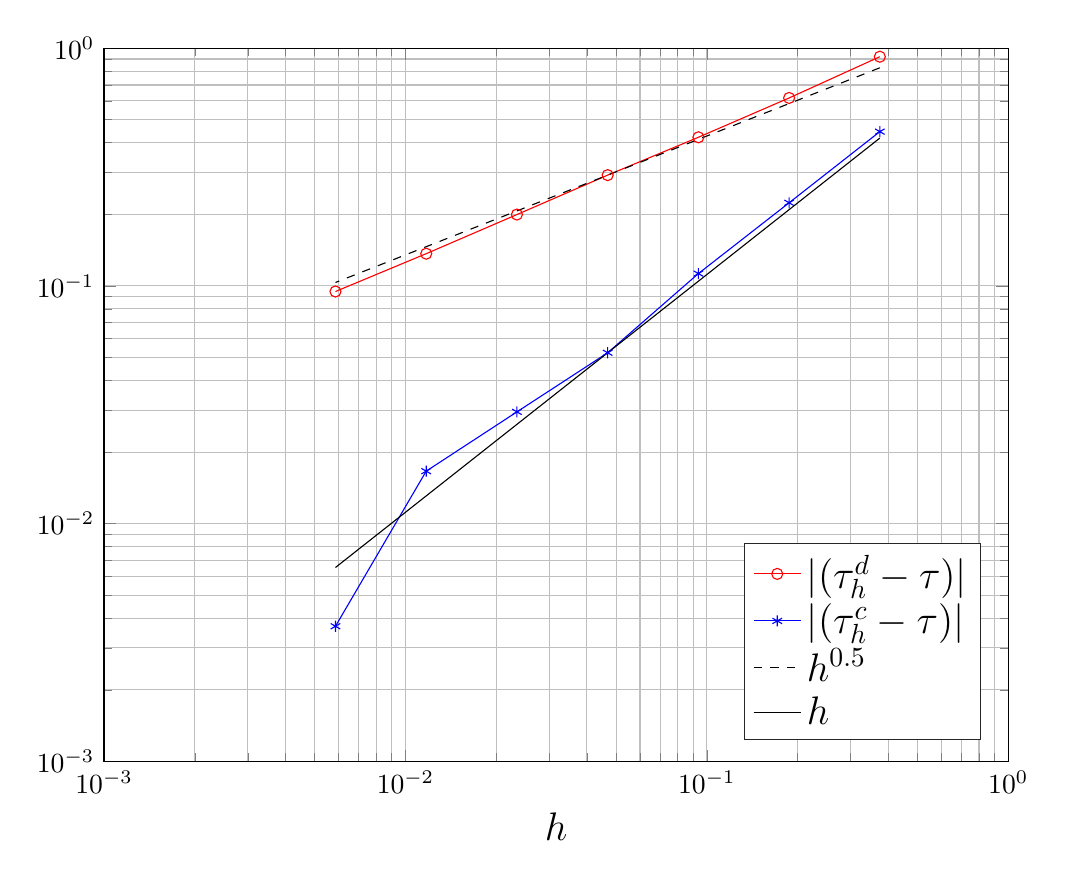
\begin{tikzpicture}

\begin{axis}[%
width=4.521in,
height=3.566in,
at={(0.758in,0.481in)},
scale only axis,
xmode=log,
xmin=0.001,
xmax=1,
xminorticks=true,
xlabel={$h$},
xlabel style={font=\Large},
xmajorgrids,
xminorgrids,
ymode=log,
ymin=0.001,
ymax=1,
yminorticks=true,
ymajorgrids,
yminorgrids,
axis background/.style={fill=white},
legend pos = south east,
legend style={legend cell align=left,align=left,draw=white!15!black,font=\Large}
]
\addplot [color=red,solid,mark=o,mark options={solid}]
  table[row sep=crcr]{%
0.375	0.920558951920583\\
0.1875	0.617333951920583\\
0.09375	0.421846451920583\\
0.046875	0.292363639420583\\
0.0234375	0.199588639420583\\
0.01171875	0.136614420670583\\
0.005859375	0.0947198894205827\\
};
\addlegendentry{$|\E(\tau_h^d - \tau)|$};

\addplot [color=blue,solid,mark=asterisk,mark options={solid}]
  table[row sep=crcr]{%
0.375	0.445546451920583\\
0.1875	0.223658951920583\\
0.09375	0.112677701920583\\
0.046875	0.0523214519205826\\
0.0234375	0.0295214519205826\\
0.01171875	0.0166261394205827\\
0.005859375	0.00370153004558271\\
};
\addlegendentry{$|\E(\tau_h^c - \tau)|$};

\addplot [color=black,dashed]
  table[row sep=crcr]{%
0.375	0.82692924802669\\
0.1875	0.584727278841165\\
0.09375	0.413464624013345\\
0.046875	0.292363639420583\\
0.0234375	0.206732312006673\\
0.01171875	0.146181819710291\\
0.005859375	0.103366156003336\\
};
\addlegendentry{$h^{0.5}$};

\addplot [color=black,solid]
  table[row sep=crcr]{%
0.375	0.418571615364661\\
0.1875	0.20928580768233\\
0.09375	0.104642903841165\\
0.046875	0.0523214519205826\\
0.0234375	0.0261607259602913\\
0.01171875	0.0130803629801456\\
0.005859375	0.00654018149007282\\
};
\addlegendentry{$h$};

\end{axis}
\end{tikzpicture}%
 }  
        \caption{Convergence of CEM and DEM.}
        \label{fig:ReflTwoD}
    \end{subfigure}
    \begin{subfigure}{0.49\linewidth}
        \centering
        \resizebox{1\linewidth}{!}{% This file was created by matlab2tikz.
%
%The latest updates can be retrieved from
%  http://www.mathworks.com/matlabcentral/fileexchange/22022-matlab2tikz-matlab2tikz
%where you can also make suggestions and rate matlab2tikz.
%
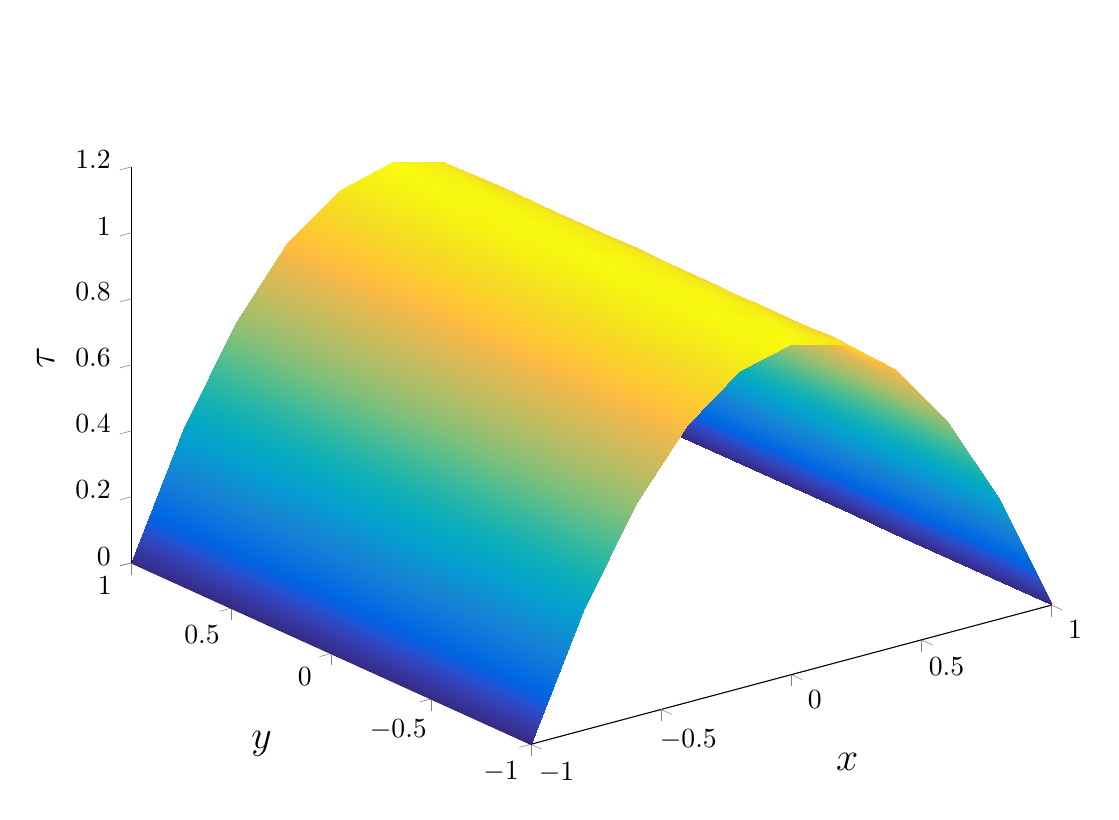
\begin{tikzpicture}

\begin{axis}[%
width=4.602in,
height=3.583in,
at={(0.772in,0.484in)},
scale only axis,
colormap={mymap}{[1pt] rgb(0pt)=(0.2081,0.1663,0.5292); rgb(1pt)=(0.211624,0.189781,0.577676); rgb(2pt)=(0.212252,0.213771,0.626971); rgb(3pt)=(0.2081,0.2386,0.677086); rgb(4pt)=(0.195905,0.264457,0.7279); rgb(5pt)=(0.170729,0.291938,0.779248); rgb(6pt)=(0.125271,0.324243,0.830271); rgb(7pt)=(0.0591333,0.359833,0.868333); rgb(8pt)=(0.0116952,0.38751,0.881957); rgb(9pt)=(0.00595714,0.408614,0.882843); rgb(10pt)=(0.0165143,0.4266,0.878633); rgb(11pt)=(0.0328524,0.443043,0.871957); rgb(12pt)=(0.0498143,0.458571,0.864057); rgb(13pt)=(0.0629333,0.47369,0.855438); rgb(14pt)=(0.0722667,0.488667,0.8467); rgb(15pt)=(0.0779429,0.503986,0.838371); rgb(16pt)=(0.0793476,0.520024,0.831181); rgb(17pt)=(0.0749429,0.537543,0.826271); rgb(18pt)=(0.0640571,0.556986,0.823957); rgb(19pt)=(0.0487714,0.577224,0.822829); rgb(20pt)=(0.0343429,0.596581,0.819852); rgb(21pt)=(0.0265,0.6137,0.8135); rgb(22pt)=(0.0238905,0.628662,0.803762); rgb(23pt)=(0.0230905,0.641786,0.791267); rgb(24pt)=(0.0227714,0.653486,0.776757); rgb(25pt)=(0.0266619,0.664195,0.760719); rgb(26pt)=(0.0383714,0.674271,0.743552); rgb(27pt)=(0.0589714,0.683757,0.725386); rgb(28pt)=(0.0843,0.692833,0.706167); rgb(29pt)=(0.113295,0.7015,0.685857); rgb(30pt)=(0.145271,0.709757,0.664629); rgb(31pt)=(0.180133,0.717657,0.642433); rgb(32pt)=(0.217829,0.725043,0.619262); rgb(33pt)=(0.258643,0.731714,0.595429); rgb(34pt)=(0.302171,0.737605,0.571186); rgb(35pt)=(0.348167,0.742433,0.547267); rgb(36pt)=(0.395257,0.7459,0.524443); rgb(37pt)=(0.44201,0.748081,0.503314); rgb(38pt)=(0.487124,0.749062,0.483976); rgb(39pt)=(0.530029,0.749114,0.466114); rgb(40pt)=(0.570857,0.748519,0.44939); rgb(41pt)=(0.609852,0.747314,0.433686); rgb(42pt)=(0.6473,0.7456,0.4188); rgb(43pt)=(0.683419,0.743476,0.404433); rgb(44pt)=(0.71841,0.741133,0.390476); rgb(45pt)=(0.752486,0.7384,0.376814); rgb(46pt)=(0.785843,0.735567,0.363271); rgb(47pt)=(0.818505,0.732733,0.34979); rgb(48pt)=(0.850657,0.7299,0.336029); rgb(49pt)=(0.882433,0.727433,0.3217); rgb(50pt)=(0.913933,0.725786,0.306276); rgb(51pt)=(0.944957,0.726114,0.288643); rgb(52pt)=(0.973895,0.731395,0.266648); rgb(53pt)=(0.993771,0.745457,0.240348); rgb(54pt)=(0.999043,0.765314,0.216414); rgb(55pt)=(0.995533,0.786057,0.196652); rgb(56pt)=(0.988,0.8066,0.179367); rgb(57pt)=(0.978857,0.827143,0.163314); rgb(58pt)=(0.9697,0.848138,0.147452); rgb(59pt)=(0.962586,0.870514,0.1309); rgb(60pt)=(0.958871,0.8949,0.113243); rgb(61pt)=(0.959824,0.921833,0.0948381); rgb(62pt)=(0.9661,0.951443,0.0755333); rgb(63pt)=(0.9763,0.9831,0.0538)},
xmin=-1,
xmax=1,
tick align=outside,
xlabel={$x$},
xlabel style={font=\Large},
ymin=-1,
ymax=1,
ylabel={$y$},
ylabel style={font=\Large},
zmin=0,
zmax=1.2,
zlabel={$\tau$},
zlabel style={font=\Large},
view={-37.5}{30},
axis background/.style={fill=white},
axis x line*=bottom,
axis y line*=left,
axis z line*=left
]

\addplot3[area legend,solid,table/row sep=crcr,patch,shader=interp,forget plot,patch table={%
0	1	2\\
3	4	5\\
6	7	8\\
9	10	11\\
12	13	14\\
15	16	17\\
18	19	20\\
21	22	23\\
24	25	26\\
27	28	29\\
30	31	32\\
33	34	35\\
36	37	38\\
39	40	41\\
42	43	44\\
45	46	47\\
48	49	50\\
51	52	53\\
54	55	56\\
57	58	59\\
60	61	62\\
63	64	65\\
66	67	68\\
69	70	71\\
72	73	74\\
75	76	77\\
78	79	80\\
81	82	83\\
84	85	86\\
87	88	89\\
90	91	92\\
93	94	95\\
96	97	98\\
99	100	101\\
102	103	104\\
105	106	107\\
108	109	110\\
111	112	113\\
114	115	116\\
117	118	119\\
120	121	122\\
123	124	125\\
126	127	128\\
129	130	131\\
132	133	134\\
135	136	137\\
138	139	140\\
141	142	143\\
144	145	146\\
147	148	149\\
150	151	152\\
153	154	155\\
156	157	158\\
159	160	161\\
162	163	164\\
165	166	167\\
168	169	170\\
171	172	173\\
174	175	176\\
177	178	179\\
180	181	182\\
183	184	185\\
186	187	188\\
189	190	191\\
192	193	194\\
195	196	197\\
198	199	200\\
201	202	203\\
204	205	206\\
207	208	209\\
210	211	212\\
213	214	215\\
216	217	218\\
219	220	221\\
222	223	224\\
225	226	227\\
228	229	230\\
231	232	233\\
234	235	236\\
237	238	239\\
240	241	242\\
243	244	245\\
246	247	248\\
249	250	251\\
252	253	254\\
255	256	257\\
258	259	260\\
261	262	263\\
264	265	266\\
267	268	269\\
270	271	272\\
273	274	275\\
276	277	278\\
279	280	281\\
282	283	284\\
285	286	287\\
288	289	290\\
291	292	293\\
294	295	296\\
297	298	299\\
300	301	302\\
303	304	305\\
306	307	308\\
309	310	311\\
312	313	314\\
315	316	317\\
318	319	320\\
321	322	323\\
324	325	326\\
327	328	329\\
330	331	332\\
333	334	335\\
336	337	338\\
339	340	341\\
342	343	344\\
345	346	347\\
348	349	350\\
351	352	353\\
354	355	356\\
357	358	359\\
360	361	362\\
363	364	365\\
366	367	368\\
369	370	371\\
372	373	374\\
375	376	377\\
378	379	380\\
381	382	383\\
384	385	386\\
387	388	389\\
390	391	392\\
393	394	395\\
396	397	398\\
399	400	401\\
402	403	404\\
405	406	407\\
408	409	410\\
411	412	413\\
414	415	416\\
417	418	419\\
420	421	422\\
423	424	425\\
426	427	428\\
429	430	431\\
432	433	434\\
435	436	437\\
438	439	440\\
441	442	443\\
444	445	446\\
447	448	449\\
450	451	452\\
453	454	455\\
456	457	458\\
459	460	461\\
462	463	464\\
465	466	467\\
468	469	470\\
471	472	473\\
474	475	476\\
477	478	479\\
480	481	482\\
483	484	485\\
486	487	488\\
489	490	491\\
492	493	494\\
495	496	497\\
498	499	500\\
501	502	503\\
504	505	506\\
507	508	509\\
510	511	512\\
513	514	515\\
516	517	518\\
519	520	521\\
522	523	524\\
525	526	527\\
528	529	530\\
531	532	533\\
534	535	536\\
537	538	539\\
540	541	542\\
543	544	545\\
546	547	548\\
549	550	551\\
552	553	554\\
555	556	557\\
558	559	560\\
561	562	563\\
564	565	566\\
567	568	569\\
570	571	572\\
573	574	575\\
576	577	578\\
579	580	581\\
582	583	584\\
585	586	587\\
588	589	590\\
591	592	593\\
594	595	596\\
597	598	599\\
600	601	602\\
603	604	605\\
606	607	608\\
609	610	611\\
612	613	614\\
615	616	617\\
618	619	620\\
621	622	623\\
624	625	626\\
627	628	629\\
630	631	632\\
633	634	635\\
636	637	638\\
639	640	641\\
642	643	644\\
645	646	647\\
648	649	650\\
651	652	653\\
654	655	656\\
657	658	659\\
660	661	662\\
663	664	665\\
666	667	668\\
669	670	671\\
672	673	674\\
675	676	677\\
678	679	680\\
681	682	683\\
684	685	686\\
687	688	689\\
690	691	692\\
693	694	695\\
696	697	698\\
699	700	701\\
702	703	704\\
705	706	707\\
708	709	710\\
711	712	713\\
714	715	716\\
717	718	719\\
720	721	722\\
723	724	725\\
726	727	728\\
729	730	731\\
732	733	734\\
735	736	737\\
738	739	740\\
741	742	743\\
744	745	746\\
747	748	749\\
750	751	752\\
753	754	755\\
756	757	758\\
759	760	761\\
762	763	764\\
765	766	767\\
768	769	770\\
771	772	773\\
774	775	776\\
777	778	779\\
780	781	782\\
783	784	785\\
786	787	788\\
789	790	791\\
792	793	794\\
795	796	797\\
798	799	800\\
801	802	803\\
804	805	806\\
807	808	809\\
810	811	812\\
813	814	815\\
816	817	818\\
819	820	821\\
822	823	824\\
825	826	827\\
828	829	830\\
831	832	833\\
834	835	836\\
837	838	839\\
840	841	842\\
843	844	845\\
846	847	848\\
849	850	851\\
852	853	854\\
855	856	857\\
858	859	860\\
861	862	863\\
864	865	866\\
867	868	869\\
870	871	872\\
873	874	875\\
876	877	878\\
879	880	881\\
882	883	884\\
885	886	887\\
888	889	890\\
891	892	893\\
894	895	896\\
897	898	899\\
900	901	902\\
903	904	905\\
906	907	908\\
909	910	911\\
912	913	914\\
915	916	917\\
918	919	920\\
921	922	923\\
924	925	926\\
927	928	929\\
930	931	932\\
933	934	935\\
}]
table[row sep=crcr, point meta=\thisrow{c}] {%
x	y	z	c\\
-0.8	1	0.360600789054301	0.360600789054301\\
-1	1	0	0\\
-0.870979864217162	0.874090623781756	0.239859277391115	0.239859277391115\\
-0.6	1	0.640491282159661	0.640491282159661\\
-0.8	1	0.360600789054301	0.360600789054301\\
-0.715759069893515	0.851783447512538	0.486496946106705	0.486496946106705\\
-0.4	1	0.841915538620754	0.841915538620754\\
-0.6	1	0.640491282159661	0.640491282159661\\
-0.553557227232278	0.85599352174284	0.692522390225689	0.692522390225689\\
-0.2	1	0.961730564647817	0.961730564647817\\
-0.4	1	0.841915538620754	0.841915538620754\\
-0.256371139537587	0.844436132195903	0.934083042087989	0.934083042087989\\
0	1	1.00284345596087	1.00284345596087\\
-0.2	1	0.961730564647817	0.961730564647817\\
-0.123171927132804	0.882407229449651	0.984158790678844	0.984158790678844\\
0.2	1	0.961368900240203	0.961368900240203\\
0	1	1.00284345596087	1.00284345596087\\
0.138576080047019	0.836444863570092	0.981193330437155	0.981193330437155\\
0.4	1	0.840760731727363	0.840760731727363\\
0.2	1	0.961368900240203	0.961368900240203\\
0.314746867281053	0.841650113118016	0.901147153165762	0.901147153165762\\
0.6	1	0.640360020804884	0.640360020804884\\
0.4	1	0.840760731727363	0.840760731727363\\
0.500557557249754	0.834821560479383	0.749201168032203	0.749201168032203\\
1	0.8	0	0\\
1	1	0	0\\
0.913245437763783	0.903908655259532	0.163805732451607	0.163805732451607\\
0.8	1	0.361493877531523	0.361493877531523\\
0.6	1	0.640360020804884	0.640360020804884\\
0.6908636124721	0.827426566529025	0.522063794642751	0.522063794642751\\
1	1	0	0\\
0.8	1	0.361493877531523	0.361493877531523\\
0.913245437763783	0.903908655259532	0.163805732451607	0.163805732451607\\
0.913245437763783	0.903908655259532	0.163805732451607	0.163805732451607\\
0.8	1	0.361493877531523	0.361493877531523\\
0.853111865010539	0.81689479082676	0.270990124964959	0.270990124964959\\
1	0.6	0	0\\
1	0.8	0	0\\
0.913257156072776	0.71766207885242	0.163230151401209	0.163230151401209\\
1	0.4	0	0\\
1	0.6	0	0\\
0.858172452446661	0.489687445107711	0.261682518030455	0.261682518030455\\
1	0.2	0	0\\
1	0.4	0	0\\
0.801876020058965	0.306586241275605	0.358544002692492	0.358544002692492\\
1	-0.2	0	0\\
1	0	0	0\\
0.842830738889788	-0.109162193087545	0.288668297301798	0.288668297301798\\
1	-0.4	0	0\\
1	-0.2	0	0\\
0.839553137409186	-0.294644298019888	0.294867736919447	0.294867736919447\\
1	-0.6	0	0\\
1	-0.4	0	0\\
0.825961266928206	-0.490102064147121	0.318608835409922	0.318608835409922\\
0.8	-1	0.361511288117814	0.361511288117814\\
1	-1	0	0\\
0.903543131650638	-0.913183857559471	0.179677948635493	0.179677948635493\\
1	-0.8	0	0\\
1	-0.6	0	0\\
0.822757598423982	-0.688930059869196	0.323681118411123	0.323681118411123\\
1	-1	0	0\\
1	-0.8	0	0\\
0.903543131650638	-0.913183857559471	0.179677948635493	0.179677948635493\\
0.903543131650638	-0.913183857559471	0.179677948635493	0.179677948635493\\
1	-0.8	0	0\\
0.815246907920555	-0.852962033044177	0.333913099068588	0.333913099068588\\
0.6	-1	0.640679825801503	0.640679825801503\\
0.8	-1	0.361511288117814	0.361511288117814\\
0.716262971529556	-0.913440138799354	0.483947882678644	0.483947882678644\\
0.4	-1	0.840779517817927	0.840779517817927\\
0.6	-1	0.640679825801503	0.640679825801503\\
0.486610676987292	-0.860815662729556	0.762434059022616	0.762434059022616\\
0.2	-1	0.960678353375381	0.960678353375381\\
0.4	-1	0.840779517817927	0.840779517817927\\
0.30415666992098	-0.806486553345674	0.909564391557416	0.909564391557416\\
-0.2	-1	0.961252352940462	0.961252352940462\\
0	-1	1.00122449995786	1.00122449995786\\
-0.108836774839956	-0.842631178463089	0.989101235372461	0.989101235372461\\
-0.4	-1	0.84054087387237	0.84054087387237\\
-0.2	-1	0.961252352940462	0.961252352940462\\
-0.295155054484333	-0.839202734226978	0.913311337508362	0.913311337508362\\
-0.6	-1	0.640424842543534	0.640424842543534\\
-0.4	-1	0.84054087387237	0.84054087387237\\
-0.491181950150036	-0.827450133500077	0.758860193106688	0.758860193106688\\
-1	-0.8	0	0\\
-1	-1	0	0\\
-0.913179600822541	-0.903978796898105	0.16404514787245	0.16404514787245\\
-0.8	-1	0.361717274493557	0.361717274493557\\
-0.6	-1	0.640424842543534	0.640424842543534\\
-0.689383148912005	-0.825669061227738	0.524631788972618	0.524631788972618\\
-1	-1	0	0\\
-0.8	-1	0.361717274493557	0.361717274493557\\
-0.913179600822541	-0.903978796898105	0.16404514787245	0.16404514787245\\
-0.913179600822541	-0.903978796898105	0.16404514787245	0.16404514787245\\
-0.8	-1	0.361717274493557	0.361717274493557\\
-0.852930471573381	-0.817084814175369	0.271555408139674	0.271555408139674\\
-1	-0.6	0	0\\
-1	-0.8	0	0\\
-0.913349182557632	-0.71824277938499	0.163203893325669	0.163203893325669\\
-1	-0.4	0	0\\
-1	-0.6	0	0\\
-0.858612569930114	-0.502582179815703	0.260853780386353	0.260853780386353\\
-1	-0.2	0	0\\
-1	-0.4	0	0\\
-0.875147249859378	-0.2495178793164	0.232618447603066	0.232618447603066\\
0.822757598423982	-0.688930059869196	0.323681118411123	0.323681118411123\\
1	-0.6	0	0\\
0.825961266928206	-0.490102064147121	0.318608835409922	0.318608835409922\\
-1	0.2	0	0\\
-1	0	0	0\\
-0.878430687062504	0.0687937548368703	0.225788638375186	0.225788638375186\\
-1	0.4	0	0\\
-1	0.2	0	0\\
-0.858638192546528	0.336283758462884	0.260561904995708	0.260561904995708\\
0.314746867281053	0.841650113118016	0.901147153165762	0.901147153165762\\
0.2	1	0.961368900240203	0.961368900240203\\
0.138576080047019	0.836444863570092	0.981193330437155	0.981193330437155\\
-1	0.6	0	0\\
-1	0.4	0	0\\
-0.81542002432126	0.514265339146589	0.336111582616146	0.336111582616146\\
-1	0	0	0\\
-1	-0.2	0	0\\
-0.849550627410001	-0.0857161204413969	0.278923893229734	0.278923893229734\\
-0.81542002432126	0.514265339146589	0.336111582616146	0.336111582616146\\
-1	0.4	0	0\\
-0.858638192546528	0.336283758462884	0.260561904995708	0.260561904995708\\
0	-1	1.00122449995786	1.00122449995786\\
0.2	-1	0.960678353375381	0.960678353375381\\
0.0842448278397462	-0.826656651009239	0.994216266348817	0.994216266348817\\
-0.295155054484333	-0.839202734226978	0.913311337508362	0.913311337508362\\
-0.2	-1	0.961252352940462	0.961252352940462\\
-0.108836774839956	-0.842631178463089	0.989101235372461	0.989101235372461\\
1	0	0	0\\
1	0.2	0	0\\
0.825000730866433	0.0840636812185947	0.319213914056299	0.319213914056299\\
0.839553137409186	-0.294644298019888	0.294867736919447	0.294867736919447\\
1	-0.2	0	0\\
0.842830738889788	-0.109162193087545	0.288668297301798	0.288668297301798\\
-0.421476522111469	0.76529746608585	0.822836734575626	0.822836734575626\\
-0.4	1	0.841915538620754	0.841915538620754\\
-0.553557227232278	0.85599352174284	0.692522390225689	0.692522390225689\\
-1	1	0	0\\
-1	0.8	0	0\\
-0.870979864217162	0.874090623781756	0.239859277391115	0.239859277391115\\
-1	0.8	0	0\\
-1	0.6	0	0\\
-0.838909094432717	0.717165597536304	0.297151196902934	0.297151196902934\\
-0.870979864217162	0.874090623781756	0.239859277391115	0.239859277391115\\
-1	0.8	0	0\\
-0.838909094432717	0.717165597536304	0.297151196902934	0.297151196902934\\
-0.689383148912005	-0.825669061227738	0.524631788972618	0.524631788972618\\
-0.6	-1	0.640424842543534	0.640424842543534\\
-0.491181950150036	-0.827450133500077	0.758860193106688	0.758860193106688\\
0.162899107774523	0.0782930267751429	0.974005215726172	0.974005215726172\\
-0.0145232187187818	0.0259493451768655	0.999205050761528	0.999205050761528\\
0.0995954131227801	-0.0711056079718885	0.988536281335325	0.988536281335325\\
0.6908636124721	0.827426566529025	0.522063794642751	0.522063794642751\\
0.6	1	0.640360020804884	0.640360020804884\\
0.500557557249754	0.834821560479383	0.749201168032203	0.749201168032203\\
-0.0437189086592884	-0.1794562797288	0.999407875924147	0.999407875924147\\
-0.0145232187187818	0.0259493451768655	0.999205050761528	0.999205050761528\\
-0.183666461200581	-0.0196981175980336	0.966126125617536	0.966126125617536\\
-0.183666461200581	-0.0196981175980336	0.966126125617536	0.966126125617536\\
-0.0145232187187818	0.0259493451768655	0.999205050761528	0.999205050761528\\
-0.143244730260345	0.15312684048721	0.979268321583401	0.979268321583401\\
-0.573742666641828	0.478792000601255	0.669119447374178	0.669119447374178\\
-0.435775856529045	0.402580883145608	0.808443041196626	0.808443041196626\\
-0.436448993108287	0.574739898722634	0.809399198789772	0.809399198789772\\
-0.777645420963466	0.191713474052978	0.396499642543184	0.396499642543184\\
-1	0.2	0	0\\
-0.878430687062504	0.0687937548368703	0.225788638375186	0.225788638375186\\
-0.308985524220196	-0.434191396690207	0.904638804118675	0.904638804118675\\
-0.44256229481138	-0.30475784338953	0.802616810542302	0.802616810542302\\
-0.504626867096141	-0.476494146294975	0.745183530905945	0.745183530905945\\
0.30415666992098	-0.806486553345674	0.909564391557416	0.909564391557416\\
0.4	-1	0.840779517817927	0.840779517817927\\
0.486610676987292	-0.860815662729556	0.762434059022616	0.762434059022616\\
0.0893690793198263	-0.463478876426208	0.991825156767633	0.991825156767633\\
0.261928641455601	-0.488055957894452	0.931707123511754	0.931707123511754\\
0.2060410026947	-0.342035240885369	0.956193171406951	0.956193171406951\\
0.801876020058965	0.306586241275605	0.358544002692492	0.358544002692492\\
1	0.4	0	0\\
0.858172452446661	0.489687445107711	0.261682518030455	0.261682518030455\\
0.500557557249754	0.834821560479383	0.749201168032203	0.749201168032203\\
0.4	1	0.840760731727363	0.840760731727363\\
0.314746867281053	0.841650113118016	0.901147153165762	0.901147153165762\\
-0.0174658545926647	0.801898927302032	0.99866022482065	0.99866022482065\\
0	1	1.00284345596087	1.00284345596087\\
-0.123171927132804	0.882407229449651	0.984158790678844	0.984158790678844\\
0.629591208237007	0.150059132096618	0.6051616820519	0.6051616820519\\
0.464005364535939	0.260203010616371	0.784232155411903	0.784232155411903\\
0.457941066948159	0.074681360252563	0.78988104270503	0.78988104270503\\
-0.536183382478912	-0.125067364855863	0.713275708382721	0.713275708382721\\
-0.44256229481138	-0.30475784338953	0.802616810542302	0.802616810542302\\
-0.376489904228021	-0.187383275146088	0.856428557335802	0.856428557335802\\
0.825961266928206	-0.490102064147121	0.318608835409922	0.318608835409922\\
1	-0.4	0	0\\
0.839553137409186	-0.294644298019888	0.294867736919447	0.294867736919447\\
-0.491181950150036	-0.827450133500077	0.758860193106688	0.758860193106688\\
-0.4	-1	0.84054087387237	0.84054087387237\\
-0.295155054484333	-0.839202734226978	0.913311337508362	0.913311337508362\\
0.151932036409303	-0.636460365815934	0.977221024462473	0.977221024462473\\
0.261928641455601	-0.488055957894452	0.931707123511754	0.931707123511754\\
0.0893690793198263	-0.463478876426208	0.991825156767633	0.991825156767633\\
-0.31111533158028	-0.281732042536466	0.900823435305982	0.900823435305982\\
-0.241660277500026	-0.172513969577467	0.94104375303322	0.94104375303322\\
-0.376489904228021	-0.187383275146088	0.856428557335802	0.856428557335802\\
-0.796122724389227	-0.361886425045465	0.366578675558219	0.366578675558219\\
-0.695084883753552	-0.495926997595022	0.516155190250719	0.516155190250719\\
-0.617615903555302	-0.32670910304294	0.617618625951112	0.617618625951112\\
0.321736948673632	-0.218404805181936	0.896441155494337	0.896441155494337\\
0.149400916774043	-0.200302697508326	0.977903731157044	0.977903731157044\\
0.2060410026947	-0.342035240885369	0.956193171406951	0.956193171406951\\
0.459725917575231	0.478817132146761	0.790069031749911	0.790069031749911\\
0.464005364535939	0.260203010616371	0.784232155411903	0.784232155411903\\
0.609248416595618	0.336700564235885	0.627389109399426	0.627389109399426\\
-0.591992818593216	-0.654470500305776	0.650535288706925	0.650535288706925\\
-0.368952164395011	-0.646051178924541	0.865159771739089	0.865159771739089\\
-0.504626867096141	-0.476494146294975	0.745183530905945	0.745183530905945\\
0.646526572158138	-0.5892372548303	0.582412304645243	0.582412304645243\\
0.647783933105589	-0.365727428795828	0.581960543118186	0.581960543118186\\
0.453484147433517	-0.490455219207141	0.796343218935013	0.796343218935013\\
-0.8	1	0.360600789054301	0.360600789054301\\
-0.870979864217162	0.874090623781756	0.239859277391115	0.239859277391115\\
-0.715759069893515	0.851783447512538	0.486496946106705	0.486496946106705\\
-0.436448993108287	0.574739898722634	0.809399198789772	0.809399198789772\\
-0.435775856529045	0.402580883145608	0.808443041196626	0.808443041196626\\
-0.305196827885855	0.481941510996423	0.90497953192299	0.90497953192299\\
0.651531723544283	-0.800304145152872	0.575505329328998	0.575505329328998\\
0.6	-1	0.640679825801503	0.640679825801503\\
0.716262971529556	-0.913440138799354	0.483947882678644	0.483947882678644\\
0.651531723544283	-0.800304145152872	0.575505329328998	0.575505329328998\\
0.822757598423982	-0.688930059869196	0.323681118411123	0.323681118411123\\
0.646526572158138	-0.5892372548303	0.582412304645243	0.582412304645243\\
0.457941066948159	0.074681360252563	0.78988104270503	0.78988104270503\\
0.464005364535939	0.260203010616371	0.784232155411903	0.784232155411903\\
0.313359205867812	0.176240487473655	0.902314503372277	0.902314503372277\\
0.799426193403826	0.656174087711846	0.362051657334271	0.362051657334271\\
1	0.6	0	0\\
0.913257156072776	0.71766207885242	0.163230151401209	0.163230151401209\\
-0.800381152695487	-0.658205081403852	0.360847392154216	0.360847392154216\\
-1	-0.6	0	0\\
-0.913349182557632	-0.71824277938499	0.163203893325669	0.163203893325669\\
-0.800381152695487	-0.658205081403852	0.360847392154216	0.360847392154216\\
-0.689383148912005	-0.825669061227738	0.524631788972618	0.524631788972618\\
-0.591992818593216	-0.654470500305776	0.650535288706925	0.650535288706925\\
-0.131538906378604	0.468005506270669	0.983664863582035	0.983664863582035\\
0.0468419620052357	0.523978954343319	0.997787191997233	0.997787191997233\\
-0.0677763280124889	0.648507972991784	0.995475124095099	0.995475124095099\\
0.172508063347201	0.422930104621211	0.969801938072441	0.969801938072441\\
0.0468419620052357	0.523978954343319	0.997787191997233	0.997787191997233\\
0.0285171270359044	0.362157622648837	0.998839239472402	0.998839239472402\\
0.453484147433517	-0.490455219207141	0.796343218935013	0.796343218935013\\
0.261928641455601	-0.488055957894452	0.931707123511754	0.931707123511754\\
0.32991065048365	-0.623943472007708	0.890313737599109	0.890313737599109\\
0.0893690793198263	-0.463478876426208	0.991825156767633	0.991825156767633\\
-0.0468923144628943	-0.37201189317892	0.995910394811523	0.995910394811523\\
-0.0519572972000214	-0.516668038614571	0.995594579092236	0.995594579092236\\
0.801876020058965	0.306586241275605	0.358544002692492	0.358544002692492\\
0.687082418720278	0.487393175878324	0.527941640690478	0.527941640690478\\
0.609248416595618	0.336700564235885	0.627389109399426	0.627389109399426\\
0.457941066948159	0.074681360252563	0.78988104270503	0.78988104270503\\
0.386220146013541	-0.0691483215457924	0.849423624075885	0.849423624075885\\
0.521855887175084	-0.0613271652026621	0.726372020364078	0.726372020364078\\
0.0893728715906334	0.678554065055819	0.991650060061569	0.991650060061569\\
0.0468419620052357	0.523978954343319	0.997787191997233	0.997787191997233\\
0.193142943255321	0.563632036809665	0.961941048929927	0.961941048929927\\
-0.467792458521678	0.219937427890346	0.782141146605041	0.782141146605041\\
-0.435775856529045	0.402580883145608	0.808443041196626	0.808443041196626\\
-0.560240270361451	0.344844062180542	0.68427035594505	0.68427035594505\\
0.0172621493060368	0.196448852647962	0.999246071249523	0.999246071249523\\
0.167453556422288	0.263155683226473	0.971886930521425	0.971886930521425\\
0.0285171270359044	0.362157622648837	0.998839239472402	0.998839239472402\\
-0.777645420963466	0.191713474052978	0.396499642543184	0.396499642543184\\
-0.617913717697813	0.079971000861777	0.618367749736385	0.618367749736385\\
-0.624616411644707	0.242665578371416	0.608546275201191	0.608546275201191\\
-0.536183382478912	-0.125067364855863	0.713275708382721	0.713275708382721\\
-0.617913717697813	0.079971000861777	0.618367749736385	0.618367749736385\\
-0.699519166874299	-0.0584145433376073	0.509307508178047	0.509307508178047\\
-0.421476522111469	0.76529746608585	0.822836734575626	0.822836734575626\\
-0.629666025324687	0.659481894250005	0.607552332385808	0.607552332385808\\
-0.436448993108287	0.574739898722634	0.809399198789772	0.809399198789772\\
-0.467792458521678	0.219937427890346	0.782141146605041	0.782141146605041\\
-0.617913717697813	0.079971000861777	0.618367749736385	0.618367749736385\\
-0.456541297467842	0.0462574378515442	0.789805427179391	0.789805427179391\\
-0.796122724389227	-0.361886425045465	0.366578675558219	0.366578675558219\\
-1	-0.4	0	0\\
-0.858612569930114	-0.502582179815703	0.260853780386353	0.260853780386353\\
0.30415666992098	-0.806486553345674	0.909564391557416	0.909564391557416\\
0.478214140797659	-0.695585476223675	0.771792139744435	0.771792139744435\\
0.32991065048365	-0.623943472007708	0.890313737599109	0.890313737599109\\
-0.350427977113875	-0.0568798710953585	0.877309622147461	0.877309622147461\\
-0.241660277500026	-0.172513969577467	0.94104375303322	0.94104375303322\\
-0.183666461200581	-0.0196981175980336	0.966126125617536	0.966126125617536\\
0.521855887175084	-0.0613271652026621	0.726372020364078	0.726372020364078\\
0.386220146013541	-0.0691483215457924	0.849423624075885	0.849423624075885\\
0.456651668322266	-0.168447833276863	0.789344615416974	0.789344615416974\\
-0.256371139537587	0.844436132195903	0.934083042087989	0.934083042087989\\
-0.251840934393812	0.65073582839654	0.937938137234837	0.937938137234837\\
-0.14310781983293	0.765817634248709	0.978490665753227	0.978490665753227\\
1	0.8	0	0\\
0.913245437763783	0.903908655259532	0.163805732451607	0.163805732451607\\
0.853111865010539	0.81689479082676	0.270990124964959	0.270990124964959\\
-0.131538906378604	0.468005506270669	0.983664863582035	0.983664863582035\\
-0.0999792356165469	0.29750658388758	0.988482208418077	0.988482208418077\\
0.0285171270359044	0.362157622648837	0.998839239472402	0.998839239472402\\
0.799426193403826	0.656174087711846	0.362051657334271	0.362051657334271\\
0.687082418720278	0.487393175878324	0.527941640690478	0.527941640690478\\
0.858172452446661	0.489687445107711	0.261682518030455	0.261682518030455\\
0.239679041234336	-0.0747988778282174	0.941281910369404	0.941281910369404\\
0.386220146013541	-0.0691483215457924	0.849423624075885	0.849423624075885\\
0.312829618686655	0.0361464359017708	0.900687642984663	0.900687642984663\\
0.651531723544283	-0.800304145152872	0.575505329328998	0.575505329328998\\
0.478214140797659	-0.695585476223675	0.771792139744435	0.771792139744435\\
0.486610676987292	-0.860815662729556	0.762434059022616	0.762434059022616\\
-0.0437189086592884	-0.1794562797288	0.999407875924147	0.999407875924147\\
-0.0468923144628943	-0.37201189317892	0.995910394811523	0.995910394811523\\
0.0706839927525276	-0.312287735493971	0.992873684588063	0.992873684588063\\
-0.617615903555302	-0.32670910304294	0.617618625951112	0.617618625951112\\
-0.695084883753552	-0.495926997595022	0.516155190250719	0.516155190250719\\
-0.504626867096141	-0.476494146294975	0.745183530905945	0.745183530905945\\
-0.308985524220196	-0.434191396690207	0.904638804118675	0.904638804118675\\
-0.368952164395011	-0.646051178924541	0.865159771739089	0.865159771739089\\
-0.188699779816531	-0.572089273359516	0.965016575917867	0.965016575917867\\
0.467892646677106	-0.300972929247376	0.780325884507073	0.780325884507073\\
0.647783933105589	-0.365727428795828	0.581960543118186	0.581960543118186\\
0.581538749766835	-0.190353470678335	0.659656229626338	0.659656229626338\\
0.321736948673632	-0.218404805181936	0.896441155494337	0.896441155494337\\
0.386220146013541	-0.0691483215457924	0.849423624075885	0.849423624075885\\
0.239679041234336	-0.0747988778282174	0.941281910369404	0.941281910369404\\
0.6908636124721	0.827426566529025	0.522063794642751	0.522063794642751\\
0.500557557249754	0.834821560479383	0.749201168032203	0.749201168032203\\
0.590963022235164	0.660549521945042	0.650593507260515	0.650593507260515\\
0.590963022235164	0.660549521945042	0.650593507260515	0.650593507260515\\
0.500557557249754	0.834821560479383	0.749201168032203	0.749201168032203\\
0.404778435204039	0.681910640519122	0.835501931894581	0.835501931894581\\
-0.838909094432717	0.717165597536304	0.297151196902934	0.297151196902934\\
-1	0.6	0	0\\
-0.81542002432126	0.514265339146589	0.336111582616146	0.336111582616146\\
-0.573742666641828	0.478792000601255	0.669119447374178	0.669119447374178\\
-0.629666025324687	0.659481894250005	0.607552332385808	0.607552332385808\\
-0.67998691843914	0.507882653342416	0.534583174440857	0.534583174440857\\
-1	-0.8	0	0\\
-0.913179600822541	-0.903978796898105	0.16404514787245	0.16404514787245\\
-0.852930471573381	-0.817084814175369	0.271555408139674	0.271555408139674\\
-0.491181950150036	-0.827450133500077	0.758860193106688	0.758860193106688\\
-0.368952164395011	-0.646051178924541	0.865159771739089	0.865159771739089\\
-0.591992818593216	-0.654470500305776	0.650535288706925	0.650535288706925\\
0.590963022235164	0.660549521945042	0.650593507260515	0.650593507260515\\
0.687082418720278	0.487393175878324	0.527941640690478	0.527941640690478\\
0.799426193403826	0.656174087711846	0.362051657334271	0.362051657334271\\
0.6908636124721	0.827426566529025	0.522063794642751	0.522063794642751\\
0.590963022235164	0.660549521945042	0.650593507260515	0.650593507260515\\
0.799426193403826	0.656174087711846	0.362051657334271	0.362051657334271\\
0.8	-1	0.361511288117814	0.361511288117814\\
0.903543131650638	-0.913183857559471	0.179677948635493	0.179677948635493\\
0.815246907920555	-0.852962033044177	0.333913099068588	0.333913099068588\\
0.825961266928206	-0.490102064147121	0.318608835409922	0.318608835409922\\
0.647783933105589	-0.365727428795828	0.581960543118186	0.581960543118186\\
0.646526572158138	-0.5892372548303	0.582412304645243	0.582412304645243\\
-0.188699779816531	-0.572089273359516	0.965016575917867	0.965016575917867\\
-0.368952164395011	-0.646051178924541	0.865159771739089	0.865159771739089\\
-0.201012514379659	-0.715085349646872	0.959262206950445	0.959262206950445\\
-0.536183382478912	-0.125067364855863	0.713275708382721	0.713275708382721\\
-0.729105054552535	-0.200822554621074	0.468604207302521	0.468604207302521\\
-0.617615903555302	-0.32670910304294	0.617618625951112	0.617618625951112\\
0.581538749766835	-0.190353470678335	0.659656229626338	0.659656229626338\\
0.647783933105589	-0.365727428795828	0.581960543118186	0.581960543118186\\
0.717419694116031	-0.201076983778939	0.482601983187922	0.482601983187922\\
0.151932036409303	-0.636460365815934	0.977221024462473	0.977221024462473\\
0.30415666992098	-0.806486553345674	0.909564391557416	0.909564391557416\\
0.32991065048365	-0.623943472007708	0.890313737599109	0.890313737599109\\
-0.0519572972000214	-0.516668038614571	0.995594579092236	0.995594579092236\\
-0.0468923144628943	-0.37201189317892	0.995910394811523	0.995910394811523\\
-0.156991111184629	-0.442497792882714	0.973539255645371	0.973539255645371\\
-0.31111533158028	-0.281732042536466	0.900823435305982	0.900823435305982\\
-0.308985524220196	-0.434191396690207	0.904638804118675	0.904638804118675\\
-0.185241010817594	-0.314270126024311	0.964509156836044	0.964509156836044\\
-0.467792458521678	0.219937427890346	0.782141146605041	0.782141146605041\\
-0.311591314295825	0.109324344546677	0.902213627361649	0.902213627361649\\
-0.270562051272334	0.305759011517556	0.927678927371092	0.927678927371092\\
0.162899107774523	0.0782930267751429	0.974005215726172	0.974005215726172\\
0.167453556422288	0.263155683226473	0.971886930521425	0.971886930521425\\
0.0172621493060368	0.196448852647962	0.999246071249523	0.999246071249523\\
0.629591208237007	0.150059132096618	0.6051616820519	0.6051616820519\\
0.801876020058965	0.306586241275605	0.358544002692492	0.358544002692492\\
0.609248416595618	0.336700564235885	0.627389109399426	0.627389109399426\\
0.314746867281053	0.841650113118016	0.901147153165762	0.901147153165762\\
0.243215438556557	0.696935801995676	0.940661157524487	0.940661157524487\\
0.404778435204039	0.681910640519122	0.835501931894581	0.835501931894581\\
-0.421476522111469	0.76529746608585	0.822836734575626	0.822836734575626\\
-0.251840934393812	0.65073582839654	0.937938137234837	0.937938137234837\\
-0.256371139537587	0.844436132195903	0.934083042087989	0.934083042087989\\
0.404778435204039	0.681910640519122	0.835501931894581	0.835501931894581\\
0.243215438556557	0.696935801995676	0.940661157524487	0.940661157524487\\
0.318221535321866	0.579996560046282	0.897713493052954	0.897713493052954\\
0.581538749766835	-0.190353470678335	0.659656229626338	0.659656229626338\\
0.671060117555799	-0.0425238644998574	0.548727835348561	0.548727835348561\\
0.521855887175084	-0.0613271652026621	0.726372020364078	0.726372020364078\\
0.842830738889788	-0.109162193087545	0.288668297301798	0.288668297301798\\
1	0	0	0\\
0.825000730866433	0.0840636812185947	0.319213914056299	0.319213914056299\\
-0.188699779816531	-0.572089273359516	0.965016575917867	0.965016575917867\\
-0.0400681817402094	-0.67007462624905	0.999631870493906	0.999631870493906\\
-0.0519572972000214	-0.516668038614571	0.995594579092236	0.995594579092236\\
-0.108836774839956	-0.842631178463089	0.989101235372461	0.989101235372461\\
0	-1	1.00122449995786	1.00122449995786\\
0.0842448278397462	-0.826656651009239	0.994216266348817	0.994216266348817\\
-0.838909094432717	0.717165597536304	0.297151196902934	0.297151196902934\\
-0.629666025324687	0.659481894250005	0.607552332385808	0.607552332385808\\
-0.715759069893515	0.851783447512538	0.486496946106705	0.486496946106705\\
-0.131538906378604	0.468005506270669	0.983664863582035	0.983664863582035\\
-0.251840934393812	0.65073582839654	0.937938137234837	0.937938137234837\\
-0.305196827885855	0.481941510996423	0.90497953192299	0.90497953192299\\
-0.573742666641828	0.478792000601255	0.669119447374178	0.669119447374178\\
-0.698784277302622	0.374550558446254	0.511260012699424	0.511260012699424\\
-0.560240270361451	0.344844062180542	0.68427035594505	0.68427035594505\\
-0.849550627410001	-0.0857161204413969	0.278923893229734	0.278923893229734\\
-1	-0.2	0	0\\
-0.875147249859378	-0.2495178793164	0.232618447603066	0.232618447603066\\
0.629591208237007	0.150059132096618	0.6051616820519	0.6051616820519\\
0.671060117555799	-0.0425238644998574	0.548727835348561	0.548727835348561\\
0.825000730866433	0.0840636812185947	0.319213914056299	0.319213914056299\\
0.647783933105589	-0.365727428795828	0.581960543118186	0.581960543118186\\
0.825961266928206	-0.490102064147121	0.318608835409922	0.318608835409922\\
0.839553137409186	-0.294644298019888	0.294867736919447	0.294867736919447\\
0.151932036409303	-0.636460365815934	0.977221024462473	0.977221024462473\\
-0.0400681817402094	-0.67007462624905	0.999631870493906	0.999631870493906\\
0.0842448278397462	-0.826656651009239	0.994216266348817	0.994216266348817\\
-0.368952164395011	-0.646051178924541	0.865159771739089	0.865159771739089\\
-0.491181950150036	-0.827450133500077	0.758860193106688	0.758860193106688\\
-0.295155054484333	-0.839202734226978	0.913311337508362	0.913311337508362\\
-0.849550627410001	-0.0857161204413969	0.278923893229734	0.278923893229734\\
-0.729105054552535	-0.200822554621074	0.468604207302521	0.468604207302521\\
-0.699519166874299	-0.0584145433376073	0.509307508178047	0.509307508178047\\
-0.270562051272334	0.305759011517556	0.927678927371092	0.927678927371092\\
-0.311591314295825	0.109324344546677	0.902213627361649	0.902213627361649\\
-0.143244730260345	0.15312684048721	0.979268321583401	0.979268321583401\\
-0.44256229481138	-0.30475784338953	0.802616810542302	0.802616810542302\\
-0.308985524220196	-0.434191396690207	0.904638804118675	0.904638804118675\\
-0.31111533158028	-0.281732042536466	0.900823435305982	0.900823435305982\\
-0.251840934393812	0.65073582839654	0.937938137234837	0.937938137234837\\
-0.421476522111469	0.76529746608585	0.822836734575626	0.822836734575626\\
-0.436448993108287	0.574739898722634	0.809399198789772	0.809399198789772\\
-0.0437189086592884	-0.1794562797288	0.999407875924147	0.999407875924147\\
0.149400916774043	-0.200302697508326	0.977903731157044	0.977903731157044\\
0.0995954131227801	-0.0711056079718885	0.988536281335325	0.988536281335325\\
0.459725917575231	0.478817132146761	0.790069031749911	0.790069031749911\\
0.29046632350991	0.478227595927983	0.914756552949991	0.914756552949991\\
0.311159739978053	0.346682633914339	0.903869398356384	0.903869398356384\\
-0.695084883753552	-0.495926997595022	0.516155190250719	0.516155190250719\\
-0.800381152695487	-0.658205081403852	0.360847392154216	0.360847392154216\\
-0.591992818593216	-0.654470500305776	0.650535288706925	0.650535288706925\\
-0.689383148912005	-0.825669061227738	0.524631788972618	0.524631788972618\\
-0.491181950150036	-0.827450133500077	0.758860193106688	0.758860193106688\\
-0.591992818593216	-0.654470500305776	0.650535288706925	0.650535288706925\\
0.478214140797659	-0.695585476223675	0.771792139744435	0.771792139744435\\
0.651531723544283	-0.800304145152872	0.575505329328998	0.575505329328998\\
0.646526572158138	-0.5892372548303	0.582412304645243	0.582412304645243\\
0.822757598423982	-0.688930059869196	0.323681118411123	0.323681118411123\\
0.825961266928206	-0.490102064147121	0.318608835409922	0.318608835409922\\
0.646526572158138	-0.5892372548303	0.582412304645243	0.582412304645243\\
-0.777645420963466	0.191713474052978	0.396499642543184	0.396499642543184\\
-0.698784277302622	0.374550558446254	0.511260012699424	0.511260012699424\\
-0.858638192546528	0.336283758462884	0.260561904995708	0.260561904995708\\
-0.629666025324687	0.659481894250005	0.607552332385808	0.607552332385808\\
-0.838909094432717	0.717165597536304	0.297151196902934	0.297151196902934\\
-0.81542002432126	0.514265339146589	0.336111582616146	0.336111582616146\\
-0.870979864217162	0.874090623781756	0.239859277391115	0.239859277391115\\
-0.838909094432717	0.717165597536304	0.297151196902934	0.297151196902934\\
-0.715759069893515	0.851783447512538	0.486496946106705	0.486496946106705\\
-0.715759069893515	0.851783447512538	0.486496946106705	0.486496946106705\\
-0.629666025324687	0.659481894250005	0.607552332385808	0.607552332385808\\
-0.553557227232278	0.85599352174284	0.692522390225689	0.692522390225689\\
-0.44256229481138	-0.30475784338953	0.802616810542302	0.802616810542302\\
-0.536183382478912	-0.125067364855863	0.713275708382721	0.713275708382721\\
-0.617615903555302	-0.32670910304294	0.617618625951112	0.617618625951112\\
-0.800381152695487	-0.658205081403852	0.360847392154216	0.360847392154216\\
-0.695084883753552	-0.495926997595022	0.516155190250719	0.516155190250719\\
-0.858612569930114	-0.502582179815703	0.260853780386353	0.260853780386353\\
-0.698784277302622	0.374550558446254	0.511260012699424	0.511260012699424\\
-0.777645420963466	0.191713474052978	0.396499642543184	0.396499642543184\\
-0.624616411644707	0.242665578371416	0.608546275201191	0.608546275201191\\
-0.81542002432126	0.514265339146589	0.336111582616146	0.336111582616146\\
-0.698784277302622	0.374550558446254	0.511260012699424	0.511260012699424\\
-0.67998691843914	0.507882653342416	0.534583174440857	0.534583174440857\\
-0.617913717697813	0.079971000861777	0.618367749736385	0.618367749736385\\
-0.777645420963466	0.191713474052978	0.396499642543184	0.396499642543184\\
-0.764656987373661	0.0391649423298058	0.413241553417644	0.413241553417644\\
-0.796122724389227	-0.361886425045465	0.366578675558219	0.366578675558219\\
-0.729105054552535	-0.200822554621074	0.468604207302521	0.468604207302521\\
-0.875147249859378	-0.2495178793164	0.232618447603066	0.232618447603066\\
0.321736948673632	-0.218404805181936	0.896441155494337	0.896441155494337\\
0.467892646677106	-0.300972929247376	0.780325884507073	0.780325884507073\\
0.456651668322266	-0.168447833276863	0.789344615416974	0.789344615416974\\
0.842830738889788	-0.109162193087545	0.288668297301798	0.288668297301798\\
0.671060117555799	-0.0425238644998574	0.548727835348561	0.548727835348561\\
0.717419694116031	-0.201076983778939	0.482601983187922	0.482601983187922\\
-0.185241010817594	-0.314270126024311	0.964509156836044	0.964509156836044\\
-0.308985524220196	-0.434191396690207	0.904638804118675	0.904638804118675\\
-0.156991111184629	-0.442497792882714	0.973539255645371	0.973539255645371\\
-0.108836774839956	-0.842631178463089	0.989101235372461	0.989101235372461\\
-0.0400681817402094	-0.67007462624905	0.999631870493906	0.999631870493906\\
-0.201012514379659	-0.715085349646872	0.959262206950445	0.959262206950445\\
0.2	-1	0.960678353375381	0.960678353375381\\
0.30415666992098	-0.806486553345674	0.909564391557416	0.909564391557416\\
0.0842448278397462	-0.826656651009239	0.994216266348817	0.994216266348817\\
-0.368952164395011	-0.646051178924541	0.865159771739089	0.865159771739089\\
-0.295155054484333	-0.839202734226978	0.913311337508362	0.913311337508362\\
-0.201012514379659	-0.715085349646872	0.959262206950445	0.959262206950445\\
1	0.2	0	0\\
0.801876020058965	0.306586241275605	0.358544002692492	0.358544002692492\\
0.825000730866433	0.0840636812185947	0.319213914056299	0.319213914056299\\
0.647783933105589	-0.365727428795828	0.581960543118186	0.581960543118186\\
0.839553137409186	-0.294644298019888	0.294867736919447	0.294867736919447\\
0.717419694116031	-0.201076983778939	0.482601983187922	0.482601983187922\\
0.459725917575231	0.478817132146761	0.790069031749911	0.790069031749911\\
0.590963022235164	0.660549521945042	0.650593507260515	0.650593507260515\\
0.404778435204039	0.681910640519122	0.835501931894581	0.835501931894581\\
0.172508063347201	0.422930104621211	0.969801938072441	0.969801938072441\\
0.29046632350991	0.478227595927983	0.914756552949991	0.914756552949991\\
0.193142943255321	0.563632036809665	0.961941048929927	0.961941048929927\\
-0.368952164395011	-0.646051178924541	0.865159771739089	0.865159771739089\\
-0.308985524220196	-0.434191396690207	0.904638804118675	0.904638804118675\\
-0.504626867096141	-0.476494146294975	0.745183530905945	0.745183530905945\\
-0.729105054552535	-0.200822554621074	0.468604207302521	0.468604207302521\\
-0.796122724389227	-0.361886425045465	0.366578675558219	0.366578675558219\\
-0.617615903555302	-0.32670910304294	0.617618625951112	0.617618625951112\\
0.687082418720278	0.487393175878324	0.527941640690478	0.527941640690478\\
0.801876020058965	0.306586241275605	0.358544002692492	0.358544002692492\\
0.858172452446661	0.489687445107711	0.261682518030455	0.261682518030455\\
1	0.6	0	0\\
0.799426193403826	0.656174087711846	0.362051657334271	0.362051657334271\\
0.858172452446661	0.489687445107711	0.261682518030455	0.261682518030455\\
0.478214140797659	-0.695585476223675	0.771792139744435	0.771792139744435\\
0.30415666992098	-0.806486553345674	0.909564391557416	0.909564391557416\\
0.486610676987292	-0.860815662729556	0.762434059022616	0.762434059022616\\
0.6	-1	0.640679825801503	0.640679825801503\\
0.651531723544283	-0.800304145152872	0.575505329328998	0.575505329328998\\
0.486610676987292	-0.860815662729556	0.762434059022616	0.762434059022616\\
0.453484147433517	-0.490455219207141	0.796343218935013	0.796343218935013\\
0.467892646677106	-0.300972929247376	0.780325884507073	0.780325884507073\\
0.342470518429332	-0.368426311537438	0.881038810494064	0.881038810494064\\
0.0995954131227801	-0.0711056079718885	0.988536281335325	0.988536281335325\\
0.149400916774043	-0.200302697508326	0.977903731157044	0.977903731157044\\
0.239679041234336	-0.0747988778282174	0.941281910369404	0.941281910369404\\
-0.8	-1	0.361717274493557	0.361717274493557\\
-0.689383148912005	-0.825669061227738	0.524631788972618	0.524631788972618\\
-0.852930471573381	-0.817084814175369	0.271555408139674	0.271555408139674\\
-0.689383148912005	-0.825669061227738	0.524631788972618	0.524631788972618\\
-0.800381152695487	-0.658205081403852	0.360847392154216	0.360847392154216\\
-0.852930471573381	-0.817084814175369	0.271555408139674	0.271555408139674\\
0.8	1	0.361493877531523	0.361493877531523\\
0.6908636124721	0.827426566529025	0.522063794642751	0.522063794642751\\
0.853111865010539	0.81689479082676	0.270990124964959	0.270990124964959\\
0.6908636124721	0.827426566529025	0.522063794642751	0.522063794642751\\
0.799426193403826	0.656174087711846	0.362051657334271	0.362051657334271\\
0.853111865010539	0.81689479082676	0.270990124964959	0.270990124964959\\
1	-0.8	0	0\\
0.822757598423982	-0.688930059869196	0.323681118411123	0.323681118411123\\
0.815246907920555	-0.852962033044177	0.333913099068588	0.333913099068588\\
0.822757598423982	-0.688930059869196	0.323681118411123	0.323681118411123\\
0.651531723544283	-0.800304145152872	0.575505329328998	0.575505329328998\\
0.815246907920555	-0.852962033044177	0.333913099068588	0.333913099068588\\
0.0172621493060368	0.196448852647962	0.999246071249523	0.999246071249523\\
-0.0999792356165469	0.29750658388758	0.988482208418077	0.988482208418077\\
-0.143244730260345	0.15312684048721	0.979268321583401	0.979268321583401\\
0.0893728715906334	0.678554065055819	0.991650060061569	0.991650060061569\\
-0.0174658545926647	0.801898927302032	0.99866022482065	0.99866022482065\\
-0.0677763280124889	0.648507972991784	0.995475124095099	0.995475124095099\\
0.30415666992098	-0.806486553345674	0.909564391557416	0.909564391557416\\
0.151932036409303	-0.636460365815934	0.977221024462473	0.977221024462473\\
0.0842448278397462	-0.826656651009239	0.994216266348817	0.994216266348817\\
-0.0400681817402094	-0.67007462624905	0.999631870493906	0.999631870493906\\
-0.108836774839956	-0.842631178463089	0.989101235372461	0.989101235372461\\
0.0842448278397462	-0.826656651009239	0.994216266348817	0.994216266348817\\
0.801876020058965	0.306586241275605	0.358544002692492	0.358544002692492\\
0.629591208237007	0.150059132096618	0.6051616820519	0.6051616820519\\
0.825000730866433	0.0840636812185947	0.319213914056299	0.319213914056299\\
0.671060117555799	-0.0425238644998574	0.548727835348561	0.548727835348561\\
0.842830738889788	-0.109162193087545	0.288668297301798	0.288668297301798\\
0.825000730866433	0.0840636812185947	0.319213914056299	0.319213914056299\\
0.342470518429332	-0.368426311537438	0.881038810494064	0.881038810494064\\
0.321736948673632	-0.218404805181936	0.896441155494337	0.896441155494337\\
0.2060410026947	-0.342035240885369	0.956193171406951	0.956193171406951\\
-0.241660277500026	-0.172513969577467	0.94104375303322	0.94104375303322\\
-0.0437189086592884	-0.1794562797288	0.999407875924147	0.999407875924147\\
-0.183666461200581	-0.0196981175980336	0.966126125617536	0.966126125617536\\
0.521855887175084	-0.0613271652026621	0.726372020364078	0.726372020364078\\
0.671060117555799	-0.0425238644998574	0.548727835348561	0.548727835348561\\
0.571417049604729	0.030140472637374	0.670966630526899	0.670966630526899\\
0.311159739978053	0.346682633914339	0.903869398356384	0.903869398356384\\
0.167453556422288	0.263155683226473	0.971886930521425	0.971886930521425\\
0.313359205867812	0.176240487473655	0.902314503372277	0.902314503372277\\
0.467892646677106	-0.300972929247376	0.780325884507073	0.780325884507073\\
0.321736948673632	-0.218404805181936	0.896441155494337	0.896441155494337\\
0.342470518429332	-0.368426311537438	0.881038810494064	0.881038810494064\\
-0.0519572972000214	-0.516668038614571	0.995594579092236	0.995594579092236\\
-0.0400681817402094	-0.67007462624905	0.999631870493906	0.999631870493906\\
0.0365478764267567	-0.57281221203974	0.995699582164407	0.995699582164407\\
0.687082418720278	0.487393175878324	0.527941640690478	0.527941640690478\\
0.590963022235164	0.660549521945042	0.650593507260515	0.650593507260515\\
0.459725917575231	0.478817132146761	0.790069031749911	0.790069031749911\\
0.193142943255321	0.563632036809665	0.961941048929927	0.961941048929927\\
0.29046632350991	0.478227595927983	0.914756552949991	0.914756552949991\\
0.318221535321866	0.579996560046282	0.897713493052954	0.897713493052954\\
-0.629666025324687	0.659481894250005	0.607552332385808	0.607552332385808\\
-0.573742666641828	0.478792000601255	0.669119447374178	0.669119447374178\\
-0.436448993108287	0.574739898722634	0.809399198789772	0.809399198789772\\
-0.270562051272334	0.305759011517556	0.927678927371092	0.927678927371092\\
-0.131538906378604	0.468005506270669	0.983664863582035	0.983664863582035\\
-0.305196827885855	0.481941510996423	0.90497953192299	0.90497953192299\\
0.647783933105589	-0.365727428795828	0.581960543118186	0.581960543118186\\
0.467892646677106	-0.300972929247376	0.780325884507073	0.780325884507073\\
0.453484147433517	-0.490455219207141	0.796343218935013	0.796343218935013\\
0.478214140797659	-0.695585476223675	0.771792139744435	0.771792139744435\\
0.646526572158138	-0.5892372548303	0.582412304645243	0.582412304645243\\
0.453484147433517	-0.490455219207141	0.796343218935013	0.796343218935013\\
-0.695084883753552	-0.495926997595022	0.516155190250719	0.516155190250719\\
-0.591992818593216	-0.654470500305776	0.650535288706925	0.650535288706925\\
-0.504626867096141	-0.476494146294975	0.745183530905945	0.745183530905945\\
-0.44256229481138	-0.30475784338953	0.802616810542302	0.802616810542302\\
-0.617615903555302	-0.32670910304294	0.617618625951112	0.617618625951112\\
-0.504626867096141	-0.476494146294975	0.745183530905945	0.745183530905945\\
0.500557557249754	0.834821560479383	0.749201168032203	0.749201168032203\\
0.314746867281053	0.841650113118016	0.901147153165762	0.901147153165762\\
0.404778435204039	0.681910640519122	0.835501931894581	0.835501931894581\\
0.29046632350991	0.478227595927983	0.914756552949991	0.914756552949991\\
0.459725917575231	0.478817132146761	0.790069031749911	0.790069031749911\\
0.318221535321866	0.579996560046282	0.897713493052954	0.897713493052954\\
0.464005364535939	0.260203010616371	0.784232155411903	0.784232155411903\\
0.629591208237007	0.150059132096618	0.6051616820519	0.6051616820519\\
0.609248416595618	0.336700564235885	0.627389109399426	0.627389109399426\\
0.687082418720278	0.487393175878324	0.527941640690478	0.527941640690478\\
0.459725917575231	0.478817132146761	0.790069031749911	0.790069031749911\\
0.609248416595618	0.336700564235885	0.627389109399426	0.627389109399426\\
-0.0677763280124889	0.648507972991784	0.995475124095099	0.995475124095099\\
-0.0174658545926647	0.801898927302032	0.99866022482065	0.99866022482065\\
-0.14310781983293	0.765817634248709	0.978490665753227	0.978490665753227\\
-0.4	1	0.841915538620754	0.841915538620754\\
-0.421476522111469	0.76529746608585	0.822836734575626	0.822836734575626\\
-0.256371139537587	0.844436132195903	0.934083042087989	0.934083042087989\\
-0.350427977113875	-0.0568798710953585	0.877309622147461	0.877309622147461\\
-0.311591314295825	0.109324344546677	0.902213627361649	0.902213627361649\\
-0.456541297467842	0.0462574378515442	0.789805427179391	0.789805427179391\\
-0.617913717697813	0.079971000861777	0.618367749736385	0.618367749736385\\
-0.536183382478912	-0.125067364855863	0.713275708382721	0.713275708382721\\
-0.456541297467842	0.0462574378515442	0.789805427179391	0.789805427179391\\
-0.435775856529045	0.402580883145608	0.808443041196626	0.808443041196626\\
-0.467792458521678	0.219937427890346	0.782141146605041	0.782141146605041\\
-0.270562051272334	0.305759011517556	0.927678927371092	0.927678927371092\\
-0.0999792356165469	0.29750658388758	0.988482208418077	0.988482208418077\\
-0.131538906378604	0.468005506270669	0.983664863582035	0.983664863582035\\
-0.270562051272334	0.305759011517556	0.927678927371092	0.927678927371092\\
0.0468419620052357	0.523978954343319	0.997787191997233	0.997787191997233\\
-0.131538906378604	0.468005506270669	0.983664863582035	0.983664863582035\\
0.0285171270359044	0.362157622648837	0.998839239472402	0.998839239472402\\
-0.0145232187187818	0.0259493451768655	0.999205050761528	0.999205050761528\\
0.162899107774523	0.0782930267751429	0.974005215726172	0.974005215726172\\
0.0172621493060368	0.196448852647962	0.999246071249523	0.999246071249523\\
-0.311591314295825	0.109324344546677	0.902213627361649	0.902213627361649\\
-0.350427977113875	-0.0568798710953585	0.877309622147461	0.877309622147461\\
-0.183666461200581	-0.0196981175980336	0.966126125617536	0.966126125617536\\
-0.0999792356165469	0.29750658388758	0.988482208418077	0.988482208418077\\
-0.270562051272334	0.305759011517556	0.927678927371092	0.927678927371092\\
-0.143244730260345	0.15312684048721	0.979268321583401	0.979268321583401\\
-0.617913717697813	0.079971000861777	0.618367749736385	0.618367749736385\\
-0.467792458521678	0.219937427890346	0.782141146605041	0.782141146605041\\
-0.624616411644707	0.242665578371416	0.608546275201191	0.608546275201191\\
-0.624616411644707	0.242665578371416	0.608546275201191	0.608546275201191\\
-0.467792458521678	0.219937427890346	0.782141146605041	0.782141146605041\\
-0.560240270361451	0.344844062180542	0.68427035594505	0.68427035594505\\
-0.251840934393812	0.65073582839654	0.937938137234837	0.937938137234837\\
-0.131538906378604	0.468005506270669	0.983664863582035	0.983664863582035\\
-0.0677763280124889	0.648507972991784	0.995475124095099	0.995475124095099\\
-0.2	1	0.961730564647817	0.961730564647817\\
-0.256371139537587	0.844436132195903	0.934083042087989	0.934083042087989\\
-0.123171927132804	0.882407229449651	0.984158790678844	0.984158790678844\\
0.467892646677106	-0.300972929247376	0.780325884507073	0.780325884507073\\
0.581538749766835	-0.190353470678335	0.659656229626338	0.659656229626338\\
0.456651668322266	-0.168447833276863	0.789344615416974	0.789344615416974\\
0.671060117555799	-0.0425238644998574	0.548727835348561	0.548727835348561\\
0.629591208237007	0.150059132096618	0.6051616820519	0.6051616820519\\
0.571417049604729	0.030140472637374	0.670966630526899	0.670966630526899\\
-0.308985524220196	-0.434191396690207	0.904638804118675	0.904638804118675\\
-0.188699779816531	-0.572089273359516	0.965016575917867	0.965016575917867\\
-0.156991111184629	-0.442497792882714	0.973539255645371	0.973539255645371\\
-0.0400681817402094	-0.67007462624905	0.999631870493906	0.999631870493906\\
0.151932036409303	-0.636460365815934	0.977221024462473	0.977221024462473\\
0.0365478764267567	-0.57281221203974	0.995699582164407	0.995699582164407\\
-1	-0.6	0	0\\
-0.800381152695487	-0.658205081403852	0.360847392154216	0.360847392154216\\
-0.858612569930114	-0.502582179815703	0.260853780386353	0.260853780386353\\
-0.695084883753552	-0.495926997595022	0.516155190250719	0.516155190250719\\
-0.796122724389227	-0.361886425045465	0.366578675558219	0.366578675558219\\
-0.858612569930114	-0.502582179815703	0.260853780386353	0.260853780386353\\
-1	0.2	0	0\\
-0.777645420963466	0.191713474052978	0.396499642543184	0.396499642543184\\
-0.858638192546528	0.336283758462884	0.260561904995708	0.260561904995708\\
-0.698784277302622	0.374550558446254	0.511260012699424	0.511260012699424\\
-0.81542002432126	0.514265339146589	0.336111582616146	0.336111582616146\\
-0.858638192546528	0.336283758462884	0.260561904995708	0.260561904995708\\
0	1	1.00284345596087	1.00284345596087\\
-0.0174658545926647	0.801898927302032	0.99866022482065	0.99866022482065\\
0.138576080047019	0.836444863570092	0.981193330437155	0.981193330437155\\
0.243215438556557	0.696935801995676	0.940661157524487	0.940661157524487\\
0.314746867281053	0.841650113118016	0.901147153165762	0.901147153165762\\
0.138576080047019	0.836444863570092	0.981193330437155	0.981193330437155\\
-0.729105054552535	-0.200822554621074	0.468604207302521	0.468604207302521\\
-0.536183382478912	-0.125067364855863	0.713275708382721	0.713275708382721\\
-0.699519166874299	-0.0584145433376073	0.509307508178047	0.509307508178047\\
-0.764656987373661	0.0391649423298058	0.413241553417644	0.413241553417644\\
-0.777645420963466	0.191713474052978	0.396499642543184	0.396499642543184\\
-0.878430687062504	0.0687937548368703	0.225788638375186	0.225788638375186\\
0.167453556422288	0.263155683226473	0.971886930521425	0.971886930521425\\
0.162899107774523	0.0782930267751429	0.974005215726172	0.974005215726172\\
0.313359205867812	0.176240487473655	0.902314503372277	0.902314503372277\\
0.464005364535939	0.260203010616371	0.784232155411903	0.784232155411903\\
0.459725917575231	0.478817132146761	0.790069031749911	0.790069031749911\\
0.311159739978053	0.346682633914339	0.903869398356384	0.903869398356384\\
0.311159739978053	0.346682633914339	0.903869398356384	0.903869398356384\\
0.29046632350991	0.478227595927983	0.914756552949991	0.914756552949991\\
0.172508063347201	0.422930104621211	0.969801938072441	0.969801938072441\\
0.167453556422288	0.263155683226473	0.971886930521425	0.971886930521425\\
0.311159739978053	0.346682633914339	0.903869398356384	0.903869398356384\\
0.172508063347201	0.422930104621211	0.969801938072441	0.969801938072441\\
-0.0437189086592884	-0.1794562797288	0.999407875924147	0.999407875924147\\
-0.241660277500026	-0.172513969577467	0.94104375303322	0.94104375303322\\
-0.185241010817594	-0.314270126024311	0.964509156836044	0.964509156836044\\
-0.350427977113875	-0.0568798710953585	0.877309622147461	0.877309622147461\\
-0.536183382478912	-0.125067364855863	0.713275708382721	0.713275708382721\\
-0.376489904228021	-0.187383275146088	0.856428557335802	0.856428557335802\\
0.313359205867812	0.176240487473655	0.902314503372277	0.902314503372277\\
0.162899107774523	0.0782930267751429	0.974005215726172	0.974005215726172\\
0.312829618686655	0.0361464359017708	0.900687642984663	0.900687642984663\\
-0.0145232187187818	0.0259493451768655	0.999205050761528	0.999205050761528\\
-0.0437189086592884	-0.1794562797288	0.999407875924147	0.999407875924147\\
0.0995954131227801	-0.0711056079718885	0.988536281335325	0.988536281335325\\
0.138576080047019	0.836444863570092	0.981193330437155	0.981193330437155\\
-0.0174658545926647	0.801898927302032	0.99866022482065	0.99866022482065\\
0.0893728715906334	0.678554065055819	0.991650060061569	0.991650060061569\\
0.243215438556557	0.696935801995676	0.940661157524487	0.940661157524487\\
0.138576080047019	0.836444863570092	0.981193330437155	0.981193330437155\\
0.0893728715906334	0.678554065055819	0.991650060061569	0.991650060061569\\
-1	0	0	0\\
-0.849550627410001	-0.0857161204413969	0.278923893229734	0.278923893229734\\
-0.878430687062504	0.0687937548368703	0.225788638375186	0.225788638375186\\
-0.849550627410001	-0.0857161204413969	0.278923893229734	0.278923893229734\\
-0.764656987373661	0.0391649423298058	0.413241553417644	0.413241553417644\\
-0.878430687062504	0.0687937548368703	0.225788638375186	0.225788638375186\\
-0.629666025324687	0.659481894250005	0.607552332385808	0.607552332385808\\
-0.421476522111469	0.76529746608585	0.822836734575626	0.822836734575626\\
-0.553557227232278	0.85599352174284	0.692522390225689	0.692522390225689\\
-0.6	1	0.640491282159661	0.640491282159661\\
-0.715759069893515	0.851783447512538	0.486496946106705	0.486496946106705\\
-0.553557227232278	0.85599352174284	0.692522390225689	0.692522390225689\\
0.671060117555799	-0.0425238644998574	0.548727835348561	0.548727835348561\\
0.581538749766835	-0.190353470678335	0.659656229626338	0.659656229626338\\
0.717419694116031	-0.201076983778939	0.482601983187922	0.482601983187922\\
0.839553137409186	-0.294644298019888	0.294867736919447	0.294867736919447\\
0.842830738889788	-0.109162193087545	0.288668297301798	0.288668297301798\\
0.717419694116031	-0.201076983778939	0.482601983187922	0.482601983187922\\
-0.0400681817402094	-0.67007462624905	0.999631870493906	0.999631870493906\\
-0.188699779816531	-0.572089273359516	0.965016575917867	0.965016575917867\\
-0.201012514379659	-0.715085349646872	0.959262206950445	0.959262206950445\\
-0.295155054484333	-0.839202734226978	0.913311337508362	0.913311337508362\\
-0.108836774839956	-0.842631178463089	0.989101235372461	0.989101235372461\\
-0.201012514379659	-0.715085349646872	0.959262206950445	0.959262206950445\\
-1	-0.4	0	0\\
-0.796122724389227	-0.361886425045465	0.366578675558219	0.366578675558219\\
-0.875147249859378	-0.2495178793164	0.232618447603066	0.232618447603066\\
-0.729105054552535	-0.200822554621074	0.468604207302521	0.468604207302521\\
-0.849550627410001	-0.0857161204413969	0.278923893229734	0.278923893229734\\
-0.875147249859378	-0.2495178793164	0.232618447603066	0.232618447603066\\
-0.852930471573381	-0.817084814175369	0.271555408139674	0.271555408139674\\
-0.800381152695487	-0.658205081403852	0.360847392154216	0.360847392154216\\
-0.913349182557632	-0.71824277938499	0.163203893325669	0.163203893325669\\
-1	-0.8	0	0\\
-0.852930471573381	-0.817084814175369	0.271555408139674	0.271555408139674\\
-0.913349182557632	-0.71824277938499	0.163203893325669	0.163203893325669\\
0.853111865010539	0.81689479082676	0.270990124964959	0.270990124964959\\
0.799426193403826	0.656174087711846	0.362051657334271	0.362051657334271\\
0.913257156072776	0.71766207885242	0.163230151401209	0.163230151401209\\
1	0.8	0	0\\
0.853111865010539	0.81689479082676	0.270990124964959	0.270990124964959\\
0.913257156072776	0.71766207885242	0.163230151401209	0.163230151401209\\
0.815246907920555	-0.852962033044177	0.333913099068588	0.333913099068588\\
0.651531723544283	-0.800304145152872	0.575505329328998	0.575505329328998\\
0.716262971529556	-0.913440138799354	0.483947882678644	0.483947882678644\\
0.8	-1	0.361511288117814	0.361511288117814\\
0.815246907920555	-0.852962033044177	0.333913099068588	0.333913099068588\\
0.716262971529556	-0.913440138799354	0.483947882678644	0.483947882678644\\
-0.629666025324687	0.659481894250005	0.607552332385808	0.607552332385808\\
-0.81542002432126	0.514265339146589	0.336111582616146	0.336111582616146\\
-0.67998691843914	0.507882653342416	0.534583174440857	0.534583174440857\\
-0.698784277302622	0.374550558446254	0.511260012699424	0.511260012699424\\
-0.573742666641828	0.478792000601255	0.669119447374178	0.669119447374178\\
-0.67998691843914	0.507882653342416	0.534583174440857	0.534583174440857\\
0.0706839927525276	-0.312287735493971	0.992873684588063	0.992873684588063\\
0.0893690793198263	-0.463478876426208	0.991825156767633	0.991825156767633\\
0.2060410026947	-0.342035240885369	0.956193171406951	0.956193171406951\\
0.261928641455601	-0.488055957894452	0.931707123511754	0.931707123511754\\
0.453484147433517	-0.490455219207141	0.796343218935013	0.796343218935013\\
0.342470518429332	-0.368426311537438	0.881038810494064	0.881038810494064\\
0.261928641455601	-0.488055957894452	0.931707123511754	0.931707123511754\\
0.151932036409303	-0.636460365815934	0.977221024462473	0.977221024462473\\
0.32991065048365	-0.623943472007708	0.890313737599109	0.890313737599109\\
0.478214140797659	-0.695585476223675	0.771792139744435	0.771792139744435\\
0.453484147433517	-0.490455219207141	0.796343218935013	0.796343218935013\\
0.32991065048365	-0.623943472007708	0.890313737599109	0.890313737599109\\
-0.123171927132804	0.882407229449651	0.984158790678844	0.984158790678844\\
-0.256371139537587	0.844436132195903	0.934083042087989	0.934083042087989\\
-0.14310781983293	0.765817634248709	0.978490665753227	0.978490665753227\\
0.0468419620052357	0.523978954343319	0.997787191997233	0.997787191997233\\
0.0893728715906334	0.678554065055819	0.991650060061569	0.991650060061569\\
-0.0677763280124889	0.648507972991784	0.995475124095099	0.995475124095099\\
-0.0145232187187818	0.0259493451768655	0.999205050761528	0.999205050761528\\
0.0172621493060368	0.196448852647962	0.999246071249523	0.999246071249523\\
-0.143244730260345	0.15312684048721	0.979268321583401	0.979268321583401\\
-0.311591314295825	0.109324344546677	0.902213627361649	0.902213627361649\\
-0.183666461200581	-0.0196981175980336	0.966126125617536	0.966126125617536\\
-0.143244730260345	0.15312684048721	0.979268321583401	0.979268321583401\\
-0.435775856529045	0.402580883145608	0.808443041196626	0.808443041196626\\
-0.573742666641828	0.478792000601255	0.669119447374178	0.669119447374178\\
-0.560240270361451	0.344844062180542	0.68427035594505	0.68427035594505\\
-0.698784277302622	0.374550558446254	0.511260012699424	0.511260012699424\\
-0.624616411644707	0.242665578371416	0.608546275201191	0.608546275201191\\
-0.560240270361451	0.344844062180542	0.68427035594505	0.68427035594505\\
0.386220146013541	-0.0691483215457924	0.849423624075885	0.849423624075885\\
0.457941066948159	0.074681360252563	0.78988104270503	0.78988104270503\\
0.312829618686655	0.0361464359017708	0.900687642984663	0.900687642984663\\
0.464005364535939	0.260203010616371	0.784232155411903	0.784232155411903\\
0.311159739978053	0.346682633914339	0.903869398356384	0.903869398356384\\
0.313359205867812	0.176240487473655	0.902314503372277	0.902314503372277\\
-0.251840934393812	0.65073582839654	0.937938137234837	0.937938137234837\\
-0.436448993108287	0.574739898722634	0.809399198789772	0.809399198789772\\
-0.305196827885855	0.481941510996423	0.90497953192299	0.90497953192299\\
-0.435775856529045	0.402580883145608	0.808443041196626	0.808443041196626\\
-0.270562051272334	0.305759011517556	0.927678927371092	0.927678927371092\\
-0.305196827885855	0.481941510996423	0.90497953192299	0.90497953192299\\
-0.311591314295825	0.109324344546677	0.902213627361649	0.902213627361649\\
-0.467792458521678	0.219937427890346	0.782141146605041	0.782141146605041\\
-0.456541297467842	0.0462574378515442	0.789805427179391	0.789805427179391\\
-0.536183382478912	-0.125067364855863	0.713275708382721	0.713275708382721\\
-0.350427977113875	-0.0568798710953585	0.877309622147461	0.877309622147461\\
-0.456541297467842	0.0462574378515442	0.789805427179391	0.789805427179391\\
-0.0468923144628943	-0.37201189317892	0.995910394811523	0.995910394811523\\
-0.0437189086592884	-0.1794562797288	0.999407875924147	0.999407875924147\\
-0.185241010817594	-0.314270126024311	0.964509156836044	0.964509156836044\\
-0.241660277500026	-0.172513969577467	0.94104375303322	0.94104375303322\\
-0.31111533158028	-0.281732042536466	0.900823435305982	0.900823435305982\\
-0.185241010817594	-0.314270126024311	0.964509156836044	0.964509156836044\\
0.149400916774043	-0.200302697508326	0.977903731157044	0.977903731157044\\
-0.0437189086592884	-0.1794562797288	0.999407875924147	0.999407875924147\\
0.0706839927525276	-0.312287735493971	0.992873684588063	0.992873684588063\\
-0.0468923144628943	-0.37201189317892	0.995910394811523	0.995910394811523\\
0.0893690793198263	-0.463478876426208	0.991825156767633	0.991825156767633\\
0.0706839927525276	-0.312287735493971	0.992873684588063	0.992873684588063\\
-0.241660277500026	-0.172513969577467	0.94104375303322	0.94104375303322\\
-0.350427977113875	-0.0568798710953585	0.877309622147461	0.877309622147461\\
-0.376489904228021	-0.187383275146088	0.856428557335802	0.856428557335802\\
-0.44256229481138	-0.30475784338953	0.802616810542302	0.802616810542302\\
-0.31111533158028	-0.281732042536466	0.900823435305982	0.900823435305982\\
-0.376489904228021	-0.187383275146088	0.856428557335802	0.856428557335802\\
-0.0999792356165469	0.29750658388758	0.988482208418077	0.988482208418077\\
0.0172621493060368	0.196448852647962	0.999246071249523	0.999246071249523\\
0.0285171270359044	0.362157622648837	0.998839239472402	0.998839239472402\\
0.167453556422288	0.263155683226473	0.971886930521425	0.971886930521425\\
0.172508063347201	0.422930104621211	0.969801938072441	0.969801938072441\\
0.0285171270359044	0.362157622648837	0.998839239472402	0.998839239472402\\
-0.764656987373661	0.0391649423298058	0.413241553417644	0.413241553417644\\
-0.849550627410001	-0.0857161204413969	0.278923893229734	0.278923893229734\\
-0.699519166874299	-0.0584145433376073	0.509307508178047	0.509307508178047\\
-0.617913717697813	0.079971000861777	0.618367749736385	0.618367749736385\\
-0.764656987373661	0.0391649423298058	0.413241553417644	0.413241553417644\\
-0.699519166874299	-0.0584145433376073	0.509307508178047	0.509307508178047\\
0.149400916774043	-0.200302697508326	0.977903731157044	0.977903731157044\\
0.321736948673632	-0.218404805181936	0.896441155494337	0.896441155494337\\
0.239679041234336	-0.0747988778282174	0.941281910369404	0.941281910369404\\
0.162899107774523	0.0782930267751429	0.974005215726172	0.974005215726172\\
0.0995954131227801	-0.0711056079718885	0.988536281335325	0.988536281335325\\
0.239679041234336	-0.0747988778282174	0.941281910369404	0.941281910369404\\
0.0468419620052357	0.523978954343319	0.997787191997233	0.997787191997233\\
0.172508063347201	0.422930104621211	0.969801938072441	0.969801938072441\\
0.193142943255321	0.563632036809665	0.961941048929927	0.961941048929927\\
0.243215438556557	0.696935801995676	0.940661157524487	0.940661157524487\\
0.0893728715906334	0.678554065055819	0.991650060061569	0.991650060061569\\
0.193142943255321	0.563632036809665	0.961941048929927	0.961941048929927\\
0.459725917575231	0.478817132146761	0.790069031749911	0.790069031749911\\
0.404778435204039	0.681910640519122	0.835501931894581	0.835501931894581\\
0.318221535321866	0.579996560046282	0.897713493052954	0.897713493052954\\
0.243215438556557	0.696935801995676	0.940661157524487	0.940661157524487\\
0.193142943255321	0.563632036809665	0.961941048929927	0.961941048929927\\
0.318221535321866	0.579996560046282	0.897713493052954	0.897713493052954\\
0.261928641455601	-0.488055957894452	0.931707123511754	0.931707123511754\\
0.342470518429332	-0.368426311537438	0.881038810494064	0.881038810494064\\
0.2060410026947	-0.342035240885369	0.956193171406951	0.956193171406951\\
0.149400916774043	-0.200302697508326	0.977903731157044	0.977903731157044\\
0.0706839927525276	-0.312287735493971	0.992873684588063	0.992873684588063\\
0.2060410026947	-0.342035240885369	0.956193171406951	0.956193171406951\\
0.386220146013541	-0.0691483215457924	0.849423624075885	0.849423624075885\\
0.321736948673632	-0.218404805181936	0.896441155494337	0.896441155494337\\
0.456651668322266	-0.168447833276863	0.789344615416974	0.789344615416974\\
0.581538749766835	-0.190353470678335	0.659656229626338	0.659656229626338\\
0.521855887175084	-0.0613271652026621	0.726372020364078	0.726372020364078\\
0.456651668322266	-0.168447833276863	0.789344615416974	0.789344615416974\\
-0.188699779816531	-0.572089273359516	0.965016575917867	0.965016575917867\\
-0.0519572972000214	-0.516668038614571	0.995594579092236	0.995594579092236\\
-0.156991111184629	-0.442497792882714	0.973539255645371	0.973539255645371\\
-0.0468923144628943	-0.37201189317892	0.995910394811523	0.995910394811523\\
-0.185241010817594	-0.314270126024311	0.964509156836044	0.964509156836044\\
-0.156991111184629	-0.442497792882714	0.973539255645371	0.973539255645371\\
0.629591208237007	0.150059132096618	0.6051616820519	0.6051616820519\\
0.457941066948159	0.074681360252563	0.78988104270503	0.78988104270503\\
0.571417049604729	0.030140472637374	0.670966630526899	0.670966630526899\\
0.457941066948159	0.074681360252563	0.78988104270503	0.78988104270503\\
0.521855887175084	-0.0613271652026621	0.726372020364078	0.726372020364078\\
0.571417049604729	0.030140472637374	0.670966630526899	0.670966630526899\\
0.151932036409303	-0.636460365815934	0.977221024462473	0.977221024462473\\
0.0893690793198263	-0.463478876426208	0.991825156767633	0.991825156767633\\
0.0365478764267567	-0.57281221203974	0.995699582164407	0.995699582164407\\
0.0893690793198263	-0.463478876426208	0.991825156767633	0.991825156767633\\
-0.0519572972000214	-0.516668038614571	0.995594579092236	0.995594579092236\\
0.0365478764267567	-0.57281221203974	0.995699582164407	0.995699582164407\\
-0.0174658545926647	0.801898927302032	0.99866022482065	0.99866022482065\\
-0.123171927132804	0.882407229449651	0.984158790678844	0.984158790678844\\
-0.14310781983293	0.765817634248709	0.978490665753227	0.978490665753227\\
-0.251840934393812	0.65073582839654	0.937938137234837	0.937938137234837\\
-0.0677763280124889	0.648507972991784	0.995475124095099	0.995475124095099\\
-0.14310781983293	0.765817634248709	0.978490665753227	0.978490665753227\\
0.457941066948159	0.074681360252563	0.78988104270503	0.78988104270503\\
0.313359205867812	0.176240487473655	0.902314503372277	0.902314503372277\\
0.312829618686655	0.0361464359017708	0.900687642984663	0.900687642984663\\
0.162899107774523	0.0782930267751429	0.974005215726172	0.974005215726172\\
0.239679041234336	-0.0747988778282174	0.941281910369404	0.941281910369404\\
0.312829618686655	0.0361464359017708	0.900687642984663	0.900687642984663\\
};
\end{axis}
\end{tikzpicture}%
 }  
        \caption{Expectation of exit time.}
        \label{fig:TauExact2DRefl}
    \end{subfigure}    
    \caption{Summary of the results for $\tau$ in the two-dimensional case with mixed boundary conditions.}
    \label{fig:OrdersTwoDRefl}
\end{figure}


\vspace{2mm}
\noindent \textbf{Estimation of the exit probability.} We consider the same simple case as for the estimation of the exit time, with $\partial D$ endowed with pure killing boundary conditions. In this case, the partial differential equation \eqref{eq:PDEPhi} reduces to
\begin{equation}\label{eq:PDEPhi2DKilling}
	\left \{
  	\begin{aligned}
	\frac{\partial}{\partial t} \Phi(x,t,T) + \frac{1}{2} \sigma^2 \Delta \Phi(x,t,T) &= 0, && \text{in } D, 0 \leq t < T,\\
	\Phi(x,t,T) &= 1, && \text{on } \partial D, 0 \leq t < T,\\
	\Phi(x,T,T) &= 0, && \text{in } D.
  	\end{aligned} \right.
\end{equation}
We solve this problem numerically with the Finite Elements Method as for \eqref{eq:PDETau2DKilling}. The solution at $t = 0$ is shown in Figure \ref{fig:PhiExact2DKill}. We verify the orders of convergence of DEM and CEM setting $X_0 = (0,0)^T , \sigma = 1, T = 1$. We consider $M = 10^6$ trajectories and $N = 2^i,i=0,\dots,5$. We then compare the Montecarlo estimation with the value of $\Phi$ in $(0,0)$, obtained by interpolation on the Finite Elements solution. The orders of convergence for this numerical experiment are shown in Figure \ref{fig:KillTwoDPhi}. The theoretical orders of convergence are confirmed in this case as well, with an average order of $0.43$ for DEM and $1.19$ for CEM.

\begin{figure}[t]
    \centering
    \begin{subfigure}{0.49\linewidth}
        \centering
        \resizebox{1\linewidth}{!}{% This file was created by matlab2tikz.
%
%The latest updates can be retrieved from
%  http://www.mathworks.com/matlabcentral/fileexchange/22022-matlab2tikz-matlab2tikz
%where you can also make suggestions and rate matlab2tikz.
%
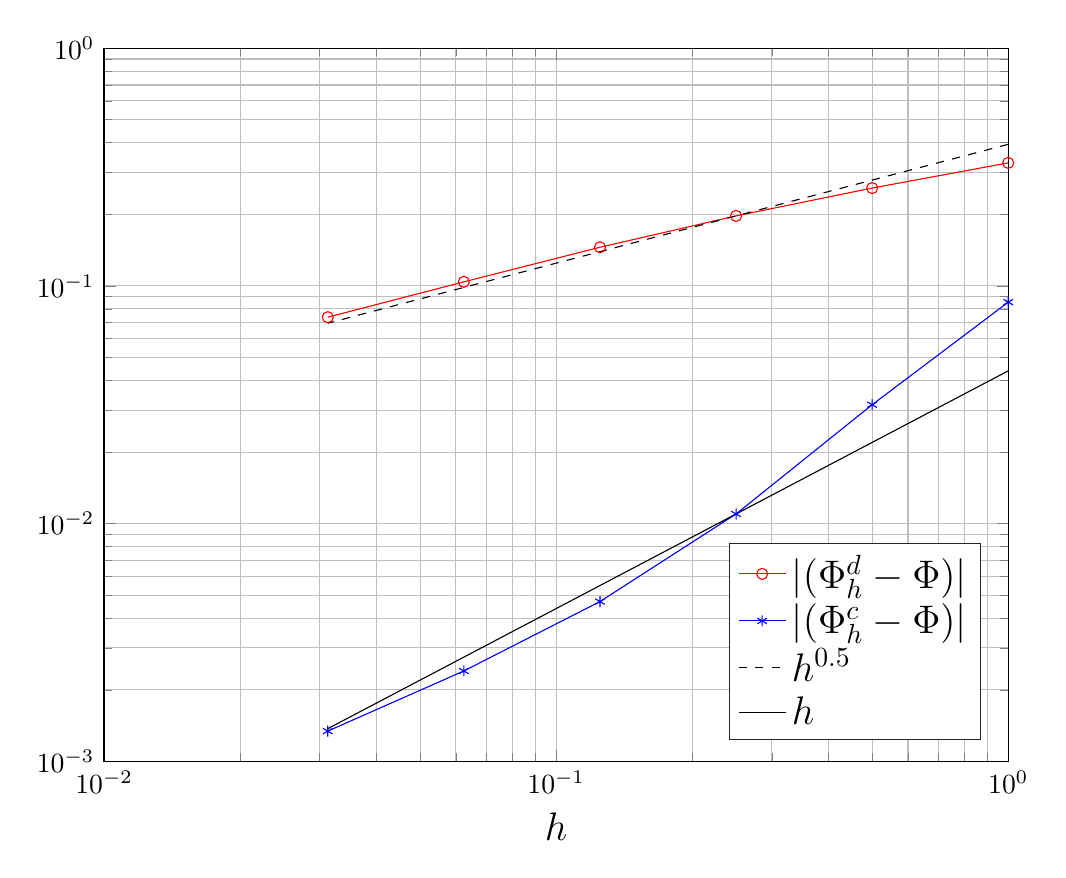
\begin{tikzpicture}

\begin{axis}[%
width=4.521in,
height=3.566in,
at={(0.758in,0.481in)},
scale only axis,
xmode=log,
xmin=0.01,
xmax=1,
xminorticks=true,
xlabel={$h$},
xlabel style={font=\Large},
xmajorgrids,
xminorgrids,
ymode=log,
ymin=0.001,
ymax=1,
yminorticks=true,
ymajorgrids,
yminorgrids,
axis background/.style={fill=white},
legend pos = south east,
legend style={legend cell align=left,align=left,draw=white!15!black,font=\Large}
]
\addplot [color=red,solid,mark=o,mark options={solid}]
  table[row sep=crcr]{%
1	0.329250554513686\\
0.5	0.257940554513686\\
0.25	0.197050554513686\\
0.125	0.145390554513686\\
0.0625	0.104000554513686\\
0.03125	0.073860554513686\\
};
\addlegendentry{$|\E(\Phi_h^d - \Phi)|$};

\addplot [color=blue,solid,mark=asterisk,mark options={solid}]
  table[row sep=crcr]{%
1	0.085450554513686\\
0.5	0.031640554513686\\
0.25	0.010980554513686\\
0.125	0.00470055451368601\\
0.0625	0.00240055451368593\\
0.03125	0.00134055451368598\\
};
\addlegendentry{$|\E(\Phi_h^c - \Phi)|$};

\addplot [color=black,dashed]
  table[row sep=crcr]{%
1	0.394101109027372\\
0.5	0.278671566666394\\
0.25	0.197050554513686\\
0.125	0.139335783333197\\
0.0625	0.098525277256843\\
0.03125	0.0696678916665984\\
};
\addlegendentry{$h^{0.5}$};

\addplot [color=black,solid]
  table[row sep=crcr]{%
1	0.0439222180547438\\
0.5	0.0219611090273719\\
0.25	0.010980554513686\\
0.125	0.00549027725684298\\
0.0625	0.00274513862842149\\
0.03125	0.00137256931421074\\
};
\addlegendentry{$h$};

\end{axis}
\end{tikzpicture}%
 }  
        \caption{Convergence of CEM and DEM.}
        \label{fig:KillTwoDPhi}
    \end{subfigure}
    \begin{subfigure}{0.49\linewidth}
        \centering
        \resizebox{1\linewidth}{!}{% This file was created by matlab2tikz.
%
%The latest updates can be retrieved from
%  http://www.mathworks.com/matlabcentral/fileexchange/22022-matlab2tikz-matlab2tikz
%where you can also make suggestions and rate matlab2tikz.
%
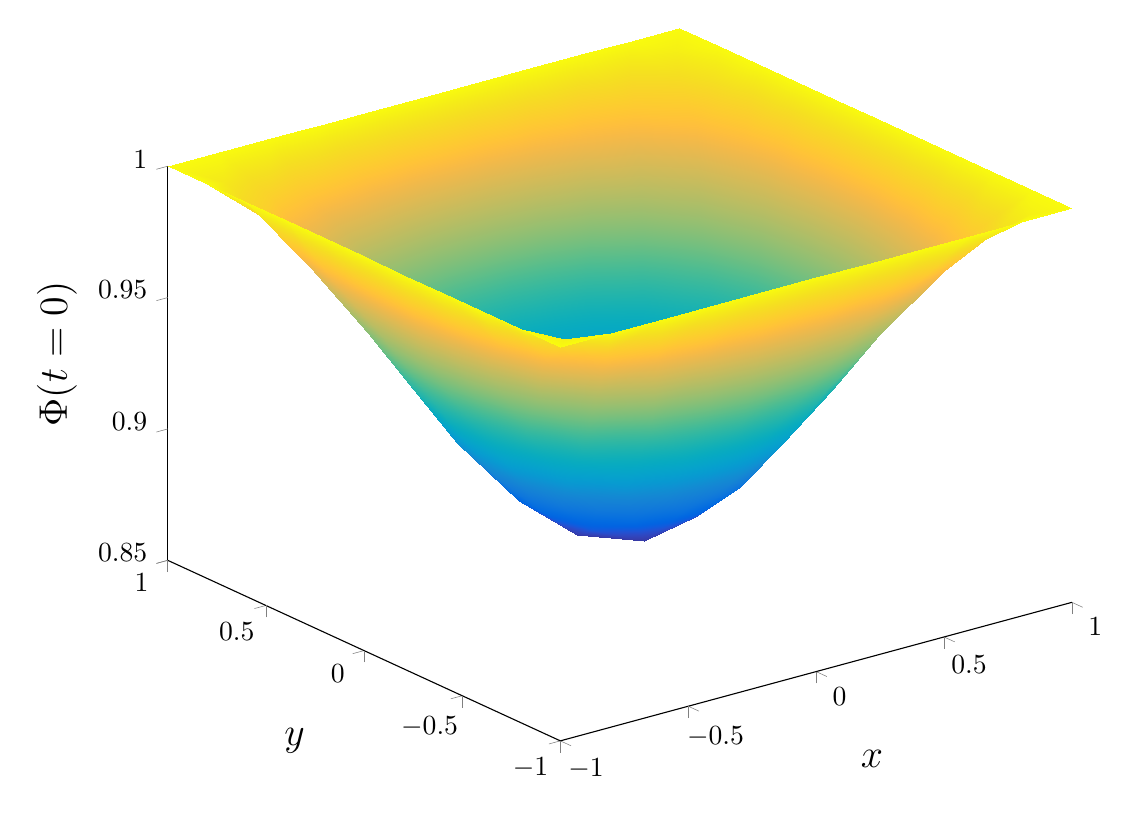
\begin{tikzpicture}

\begin{axis}[%
width=4.521in,
height=3.566in,
at={(0.758in,0.481in)},
scale only axis,
colormap={mymap}{[1pt] rgb(0pt)=(0.2081,0.1663,0.5292); rgb(1pt)=(0.211624,0.189781,0.577676); rgb(2pt)=(0.212252,0.213771,0.626971); rgb(3pt)=(0.2081,0.2386,0.677086); rgb(4pt)=(0.195905,0.264457,0.7279); rgb(5pt)=(0.170729,0.291938,0.779248); rgb(6pt)=(0.125271,0.324243,0.830271); rgb(7pt)=(0.0591333,0.359833,0.868333); rgb(8pt)=(0.0116952,0.38751,0.881957); rgb(9pt)=(0.00595714,0.408614,0.882843); rgb(10pt)=(0.0165143,0.4266,0.878633); rgb(11pt)=(0.0328524,0.443043,0.871957); rgb(12pt)=(0.0498143,0.458571,0.864057); rgb(13pt)=(0.0629333,0.47369,0.855438); rgb(14pt)=(0.0722667,0.488667,0.8467); rgb(15pt)=(0.0779429,0.503986,0.838371); rgb(16pt)=(0.0793476,0.520024,0.831181); rgb(17pt)=(0.0749429,0.537543,0.826271); rgb(18pt)=(0.0640571,0.556986,0.823957); rgb(19pt)=(0.0487714,0.577224,0.822829); rgb(20pt)=(0.0343429,0.596581,0.819852); rgb(21pt)=(0.0265,0.6137,0.8135); rgb(22pt)=(0.0238905,0.628662,0.803762); rgb(23pt)=(0.0230905,0.641786,0.791267); rgb(24pt)=(0.0227714,0.653486,0.776757); rgb(25pt)=(0.0266619,0.664195,0.760719); rgb(26pt)=(0.0383714,0.674271,0.743552); rgb(27pt)=(0.0589714,0.683757,0.725386); rgb(28pt)=(0.0843,0.692833,0.706167); rgb(29pt)=(0.113295,0.7015,0.685857); rgb(30pt)=(0.145271,0.709757,0.664629); rgb(31pt)=(0.180133,0.717657,0.642433); rgb(32pt)=(0.217829,0.725043,0.619262); rgb(33pt)=(0.258643,0.731714,0.595429); rgb(34pt)=(0.302171,0.737605,0.571186); rgb(35pt)=(0.348167,0.742433,0.547267); rgb(36pt)=(0.395257,0.7459,0.524443); rgb(37pt)=(0.44201,0.748081,0.503314); rgb(38pt)=(0.487124,0.749062,0.483976); rgb(39pt)=(0.530029,0.749114,0.466114); rgb(40pt)=(0.570857,0.748519,0.44939); rgb(41pt)=(0.609852,0.747314,0.433686); rgb(42pt)=(0.6473,0.7456,0.4188); rgb(43pt)=(0.683419,0.743476,0.404433); rgb(44pt)=(0.71841,0.741133,0.390476); rgb(45pt)=(0.752486,0.7384,0.376814); rgb(46pt)=(0.785843,0.735567,0.363271); rgb(47pt)=(0.818505,0.732733,0.34979); rgb(48pt)=(0.850657,0.7299,0.336029); rgb(49pt)=(0.882433,0.727433,0.3217); rgb(50pt)=(0.913933,0.725786,0.306276); rgb(51pt)=(0.944957,0.726114,0.288643); rgb(52pt)=(0.973895,0.731395,0.266648); rgb(53pt)=(0.993771,0.745457,0.240348); rgb(54pt)=(0.999043,0.765314,0.216414); rgb(55pt)=(0.995533,0.786057,0.196652); rgb(56pt)=(0.988,0.8066,0.179367); rgb(57pt)=(0.978857,0.827143,0.163314); rgb(58pt)=(0.9697,0.848138,0.147452); rgb(59pt)=(0.962586,0.870514,0.1309); rgb(60pt)=(0.958871,0.8949,0.113243); rgb(61pt)=(0.959824,0.921833,0.0948381); rgb(62pt)=(0.9661,0.951443,0.0755333); rgb(63pt)=(0.9763,0.9831,0.0538)},
xmin=-1,
xmax=1,
tick align=outside,
xlabel={$x$},
xlabel style = {font=\Large},
ymin=-1,
ymax=1,
ylabel={$y$},
ylabel style={font=\Large},
zmin=0.85,
zmax=1,
zlabel={$\Phi(t=0)$},
zlabel style={font=\Large},
view={-37.5}{30},
axis background/.style={fill=white},
axis x line*=bottom,
axis y line*=left,
axis z line*=left
]

\addplot3[area legend,solid,table/row sep=crcr,patch,shader=interp,forget plot,patch table={%
0	1	2\\
3	4	5\\
6	7	8\\
9	10	11\\
12	13	14\\
15	16	17\\
18	19	20\\
21	22	23\\
24	25	26\\
27	28	29\\
30	31	32\\
33	34	35\\
36	37	38\\
39	40	41\\
42	43	44\\
45	46	47\\
48	49	50\\
51	52	53\\
54	55	56\\
57	58	59\\
60	61	62\\
63	64	65\\
66	67	68\\
69	70	71\\
72	73	74\\
75	76	77\\
78	79	80\\
81	82	83\\
84	85	86\\
87	88	89\\
90	91	92\\
93	94	95\\
96	97	98\\
99	100	101\\
102	103	104\\
105	106	107\\
108	109	110\\
111	112	113\\
114	115	116\\
117	118	119\\
120	121	122\\
123	124	125\\
126	127	128\\
129	130	131\\
132	133	134\\
135	136	137\\
138	139	140\\
141	142	143\\
144	145	146\\
147	148	149\\
150	151	152\\
153	154	155\\
156	157	158\\
159	160	161\\
162	163	164\\
165	166	167\\
168	169	170\\
171	172	173\\
174	175	176\\
177	178	179\\
180	181	182\\
183	184	185\\
186	187	188\\
189	190	191\\
192	193	194\\
195	196	197\\
198	199	200\\
201	202	203\\
204	205	206\\
207	208	209\\
210	211	212\\
213	214	215\\
216	217	218\\
219	220	221\\
222	223	224\\
225	226	227\\
228	229	230\\
231	232	233\\
234	235	236\\
237	238	239\\
240	241	242\\
243	244	245\\
246	247	248\\
249	250	251\\
252	253	254\\
255	256	257\\
258	259	260\\
261	262	263\\
264	265	266\\
267	268	269\\
270	271	272\\
273	274	275\\
276	277	278\\
279	280	281\\
282	283	284\\
285	286	287\\
288	289	290\\
291	292	293\\
294	295	296\\
297	298	299\\
300	301	302\\
303	304	305\\
306	307	308\\
309	310	311\\
312	313	314\\
315	316	317\\
318	319	320\\
321	322	323\\
324	325	326\\
327	328	329\\
330	331	332\\
333	334	335\\
336	337	338\\
339	340	341\\
342	343	344\\
345	346	347\\
348	349	350\\
351	352	353\\
354	355	356\\
357	358	359\\
360	361	362\\
363	364	365\\
366	367	368\\
369	370	371\\
372	373	374\\
375	376	377\\
378	379	380\\
381	382	383\\
384	385	386\\
387	388	389\\
390	391	392\\
393	394	395\\
396	397	398\\
399	400	401\\
402	403	404\\
405	406	407\\
408	409	410\\
411	412	413\\
414	415	416\\
417	418	419\\
420	421	422\\
423	424	425\\
426	427	428\\
429	430	431\\
432	433	434\\
435	436	437\\
438	439	440\\
441	442	443\\
444	445	446\\
447	448	449\\
450	451	452\\
453	454	455\\
456	457	458\\
459	460	461\\
462	463	464\\
465	466	467\\
468	469	470\\
471	472	473\\
474	475	476\\
477	478	479\\
480	481	482\\
483	484	485\\
486	487	488\\
489	490	491\\
492	493	494\\
495	496	497\\
498	499	500\\
501	502	503\\
504	505	506\\
507	508	509\\
510	511	512\\
513	514	515\\
516	517	518\\
519	520	521\\
522	523	524\\
525	526	527\\
528	529	530\\
531	532	533\\
534	535	536\\
537	538	539\\
540	541	542\\
543	544	545\\
546	547	548\\
549	550	551\\
552	553	554\\
555	556	557\\
558	559	560\\
561	562	563\\
564	565	566\\
567	568	569\\
570	571	572\\
573	574	575\\
576	577	578\\
579	580	581\\
582	583	584\\
585	586	587\\
588	589	590\\
591	592	593\\
594	595	596\\
597	598	599\\
600	601	602\\
603	604	605\\
606	607	608\\
609	610	611\\
612	613	614\\
615	616	617\\
618	619	620\\
621	622	623\\
624	625	626\\
627	628	629\\
630	631	632\\
633	634	635\\
636	637	638\\
639	640	641\\
642	643	644\\
645	646	647\\
648	649	650\\
651	652	653\\
654	655	656\\
657	658	659\\
660	661	662\\
663	664	665\\
666	667	668\\
669	670	671\\
672	673	674\\
675	676	677\\
678	679	680\\
681	682	683\\
684	685	686\\
687	688	689\\
690	691	692\\
693	694	695\\
696	697	698\\
699	700	701\\
702	703	704\\
705	706	707\\
708	709	710\\
711	712	713\\
714	715	716\\
717	718	719\\
720	721	722\\
723	724	725\\
726	727	728\\
729	730	731\\
732	733	734\\
735	736	737\\
738	739	740\\
741	742	743\\
744	745	746\\
747	748	749\\
750	751	752\\
753	754	755\\
756	757	758\\
759	760	761\\
762	763	764\\
765	766	767\\
768	769	770\\
771	772	773\\
774	775	776\\
777	778	779\\
780	781	782\\
783	784	785\\
786	787	788\\
789	790	791\\
792	793	794\\
795	796	797\\
798	799	800\\
801	802	803\\
804	805	806\\
807	808	809\\
810	811	812\\
813	814	815\\
816	817	818\\
819	820	821\\
822	823	824\\
825	826	827\\
828	829	830\\
831	832	833\\
834	835	836\\
837	838	839\\
840	841	842\\
843	844	845\\
846	847	848\\
849	850	851\\
852	853	854\\
855	856	857\\
858	859	860\\
861	862	863\\
864	865	866\\
867	868	869\\
870	871	872\\
873	874	875\\
876	877	878\\
879	880	881\\
882	883	884\\
885	886	887\\
888	889	890\\
891	892	893\\
894	895	896\\
897	898	899\\
900	901	902\\
903	904	905\\
906	907	908\\
909	910	911\\
912	913	914\\
915	916	917\\
918	919	920\\
921	922	923\\
924	925	926\\
927	928	929\\
930	931	932\\
933	934	935\\
}]
table[row sep=crcr, point meta=\thisrow{c}] {%
x	y	z	c\\
-0.8	1	1	1\\
-1	1	1	1\\
-0.870979864217162	0.874090623781756	0.994900837726379	0.994900837726379\\
-0.6	1	1	1\\
-0.8	1	1	1\\
-0.715759069893515	0.851783447512538	0.98676550492405	0.98676550492405\\
-0.4	1	1	1\\
-0.6	1	1	1\\
-0.553557227232278	0.85599352174284	0.98067301275533	0.98067301275533\\
-0.2	1	1	1\\
-0.4	1	1	1\\
-0.256371139537587	0.844436132195903	0.970613925501264	0.970613925501264\\
0	1	1	1\\
-0.2	1	1	1\\
-0.123171927132804	0.882407229449651	0.976271284529154	0.976271284529154\\
0.2	1	1	1\\
0	1	1	1\\
0.138576080047019	0.836444863570092	0.96718109036119	0.96718109036119\\
0.4	1	1	1\\
0.2	1	1	1\\
0.314746867281053	0.841650113118016	0.971244672546017	0.971244672546017\\
0.6	1	1	1\\
0.4	1	1	1\\
0.500557557249754	0.834821560479383	0.975897428674888	0.975897428674888\\
1	0.8	1	1\\
1	1	1	1\\
0.913245437763783	0.903908655259532	0.997293344589815	0.997293344589815\\
0.8	1	1	1\\
0.6	1	1	1\\
0.6908636124721	0.827426566529025	0.983406646219684	0.983406646219684\\
1	1	1	1\\
0.8	1	1	1\\
0.913245437763783	0.903908655259532	0.997293344589815	0.997293344589815\\
0.913245437763783	0.903908655259532	0.997293344589815	0.997293344589815\\
0.8	1	1	1\\
0.853111865010539	0.81689479082676	0.991331631283587	0.991331631283587\\
1	0.6	1	1\\
1	0.8	1	1\\
0.913257156072776	0.71766207885242	0.992249980519293	0.992249980519293\\
1	0.4	1	1\\
1	0.6	1	1\\
0.858172452446661	0.489687445107711	0.978931416261557	0.978931416261557\\
1	0.2	1	1\\
1	0.4	1	1\\
0.801876020058965	0.306586241275605	0.963819950493757	0.963819950493757\\
1	-0.2	1	1\\
1	0	1	1\\
0.842830738889788	-0.109162193087545	0.968151883748015	0.968151883748015\\
1	-0.4	1	1\\
1	-0.2	1	1\\
0.839553137409186	-0.294644298019888	0.970332773422549	0.970332773422549\\
1	-0.6	1	1\\
1	-0.4	1	1\\
0.825961266928206	-0.490102064147121	0.974309290789402	0.974309290789402\\
0.8	-1	1	1\\
1	-1	1	1\\
0.903543131650638	-0.913183857559471	0.997280162089009	0.997280162089009\\
1	-0.8	1	1\\
1	-0.6	1	1\\
0.822757598423982	-0.688930059869196	0.982870705844679	0.982870705844679\\
1	-1	1	1\\
1	-0.8	1	1\\
0.903543131650638	-0.913183857559471	0.997280162089009	0.997280162089009\\
0.903543131650638	-0.913183857559471	0.997280162089009	0.997280162089009\\
1	-0.8	1	1\\
0.815246907920555	-0.852962033044177	0.991224519889577	0.991224519889577\\
0.6	-1	1	1\\
0.8	-1	1	1\\
0.716262971529556	-0.913440138799354	0.992201811500356	0.992201811500356\\
0.4	-1	1	1\\
0.6	-1	1	1\\
0.486610676987292	-0.860815662729556	0.979180011966515	0.979180011966515\\
0.2	-1	1	1\\
0.4	-1	1	1\\
0.30415666992098	-0.806486553345674	0.964572648989551	0.964572648989551\\
-0.2	-1	1	1\\
0	-1	1	1\\
-0.108836774839956	-0.842631178463089	0.968104206702289	0.968104206702289\\
-0.4	-1	1	1\\
-0.2	-1	1	1\\
-0.295155054484333	-0.839202734226978	0.970290719712475	0.970290719712475\\
-0.6	-1	1	1\\
-0.4	-1	1	1\\
-0.491181950150036	-0.827450133500077	0.974605590135046	0.974605590135046\\
-1	-0.8	1	1\\
-1	-1	1	1\\
-0.913179600822541	-0.903978796898105	0.997285844316782	0.997285844316782\\
-0.8	-1	1	1\\
-0.6	-1	1	1\\
-0.689383148912005	-0.825669061227738	0.983178068811281	0.983178068811281\\
-1	-1	1	1\\
-0.8	-1	1	1\\
-0.913179600822541	-0.903978796898105	0.997285844316782	0.997285844316782\\
-0.913179600822541	-0.903978796898105	0.997285844316782	0.997285844316782\\
-0.8	-1	1	1\\
-0.852930471573381	-0.817084814175369	0.99130925528688	0.99130925528688\\
-1	-0.6	1	1\\
-1	-0.8	1	1\\
-0.913349182557632	-0.71824277938499	0.992270278388791	0.992270278388791\\
-1	-0.4	1	1\\
-1	-0.6	1	1\\
-0.858612569930114	-0.502582179815703	0.97936622817875	0.97936622817875\\
-1	-0.2	1	1\\
-1	-0.4	1	1\\
-0.875147249859378	-0.2495178793164	0.976260703864056	0.976260703864056\\
0.822757598423982	-0.688930059869196	0.982870705844679	0.982870705844679\\
1	-0.6	1	1\\
0.825961266928206	-0.490102064147121	0.974309290789402	0.974309290789402\\
-1	0.2	1	1\\
-1	0	1	1\\
-0.878430687062504	0.0687937548368703	0.97513912998771	0.97513912998771\\
-1	0.4	1	1\\
-1	0.2	1	1\\
-0.858638192546528	0.336283758462884	0.974938148517588	0.974938148517588\\
0.314746867281053	0.841650113118016	0.971244672546017	0.971244672546017\\
0.2	1	1	1\\
0.138576080047019	0.836444863570092	0.96718109036119	0.96718109036119\\
-1	0.6	1	1\\
-1	0.4	1	1\\
-0.81542002432126	0.514265339146589	0.973484087503461	0.973484087503461\\
-1	0	1	1\\
-1	-0.2	1	1\\
-0.849550627410001	-0.0857161204413969	0.969276748763463	0.969276748763463\\
-0.81542002432126	0.514265339146589	0.973484087503461	0.973484087503461\\
-1	0.4	1	1\\
-0.858638192546528	0.336283758462884	0.974938148517588	0.974938148517588\\
0	-1	1	1\\
0.2	-1	1	1\\
0.0842448278397462	-0.826656651009239	0.964646736627235	0.964646736627235\\
-0.295155054484333	-0.839202734226978	0.970290719712475	0.970290719712475\\
-0.2	-1	1	1\\
-0.108836774839956	-0.842631178463089	0.968104206702289	0.968104206702289\\
1	0	1	1\\
1	0.2	1	1\\
0.825000730866433	0.0840636812185947	0.964317376856716	0.964317376856716\\
0.839553137409186	-0.294644298019888	0.970332773422549	0.970332773422549\\
1	-0.2	1	1\\
0.842830738889788	-0.109162193087545	0.968151883748015	0.968151883748015\\
-0.421476522111469	0.76529746608585	0.962144255721489	0.962144255721489\\
-0.4	1	1	1\\
-0.553557227232278	0.85599352174284	0.98067301275533	0.98067301275533\\
-1	1	1	1\\
-1	0.8	1	1\\
-0.870979864217162	0.874090623781756	0.994900837726379	0.994900837726379\\
-1	0.8	1	1\\
-1	0.6	1	1\\
-0.838909094432717	0.717165597536304	0.985693767813085	0.985693767813085\\
-0.870979864217162	0.874090623781756	0.994900837726379	0.994900837726379\\
-1	0.8	1	1\\
-0.838909094432717	0.717165597536304	0.985693767813085	0.985693767813085\\
-0.689383148912005	-0.825669061227738	0.983178068811281	0.983178068811281\\
-0.6	-1	1	1\\
-0.491181950150036	-0.827450133500077	0.974605590135046	0.974605590135046\\
0.162899107774523	0.0782930267751429	0.872742439565376	0.872742439565376\\
-0.0145232187187818	0.0259493451768655	0.867789035029159	0.867789035029159\\
0.0995954131227801	-0.0711056079718885	0.870504568793608	0.870504568793608\\
0.6908636124721	0.827426566529025	0.983406646219684	0.983406646219684\\
0.6	1	1	1\\
0.500557557249754	0.834821560479383	0.975897428674888	0.975897428674888\\
-0.0437189086592884	-0.1794562797288	0.87256194036436	0.87256194036436\\
-0.0145232187187818	0.0259493451768655	0.867789035029159	0.867789035029159\\
-0.183666461200581	-0.0196981175980336	0.873147501411437	0.873147501411437\\
-0.183666461200581	-0.0196981175980336	0.873147501411437	0.873147501411437\\
-0.0145232187187818	0.0259493451768655	0.867789035029159	0.867789035029159\\
-0.143244730260345	0.15312684048721	0.8747397674553	0.8747397674553\\
-0.573742666641828	0.478792000601255	0.94013688725324	0.94013688725324\\
-0.435775856529045	0.402580883145608	0.917493027129057	0.917493027129057\\
-0.436448993108287	0.574739898722634	0.936632614165645	0.936632614165645\\
-0.777645420963466	0.191713474052978	0.9567401595428	0.9567401595428\\
-1	0.2	1	1\\
-0.878430687062504	0.0687937548368703	0.97513912998771	0.97513912998771\\
-0.308985524220196	-0.434191396690207	0.90902950197148	0.90902950197148\\
-0.44256229481138	-0.30475784338953	0.909723124538403	0.909723124538403\\
-0.504626867096141	-0.476494146294975	0.93173214285744	0.93173214285744\\
0.30415666992098	-0.806486553345674	0.964572648989551	0.964572648989551\\
0.4	-1	1	1\\
0.486610676987292	-0.860815662729556	0.979180011966515	0.979180011966515\\
0.0893690793198263	-0.463478876426208	0.90220023494353	0.90220023494353\\
0.261928641455601	-0.488055957894452	0.912657925264648	0.912657925264648\\
0.2060410026947	-0.342035240885369	0.892345370672627	0.892345370672627\\
0.801876020058965	0.306586241275605	0.963819950493757	0.963819950493757\\
1	0.4	1	1\\
0.858172452446661	0.489687445107711	0.978931416261557	0.978931416261557\\
0.500557557249754	0.834821560479383	0.975897428674888	0.975897428674888\\
0.4	1	1	1\\
0.314746867281053	0.841650113118016	0.971244672546017	0.971244672546017\\
-0.0174658545926647	0.801898927302032	0.959585165793654	0.959585165793654\\
0	1	1	1\\
-0.123171927132804	0.882407229449651	0.976271284529154	0.976271284529154\\
0.629591208237007	0.150059132096618	0.929130478486791	0.929130478486791\\
0.464005364535939	0.260203010616371	0.909336169977326	0.909336169977326\\
0.457941066948159	0.074681360252563	0.901147721016767	0.901147721016767\\
-0.536183382478912	-0.125067364855863	0.913131201655364	0.913131201655364\\
-0.44256229481138	-0.30475784338953	0.909723124538403	0.909723124538403\\
-0.376489904228021	-0.187383275146088	0.895309106052268	0.895309106052268\\
0.825961266928206	-0.490102064147121	0.974309290789402	0.974309290789402\\
1	-0.4	1	1\\
0.839553137409186	-0.294644298019888	0.970332773422549	0.970332773422549\\
-0.491181950150036	-0.827450133500077	0.974605590135046	0.974605590135046\\
-0.4	-1	1	1\\
-0.295155054484333	-0.839202734226978	0.970290719712475	0.970290719712475\\
0.151932036409303	-0.636460365815934	0.930371299389602	0.930371299389602\\
0.261928641455601	-0.488055957894452	0.912657925264648	0.912657925264648\\
0.0893690793198263	-0.463478876426208	0.90220023494353	0.90220023494353\\
-0.31111533158028	-0.281732042536466	0.894897915733725	0.894897915733725\\
-0.241660277500026	-0.172513969577467	0.881749240369071	0.881749240369071\\
-0.376489904228021	-0.187383275146088	0.895309106052268	0.895309106052268\\
-0.796122724389227	-0.361886425045465	0.964838218238696	0.964838218238696\\
-0.695084883753552	-0.495926997595022	0.956478867662404	0.956478867662404\\
-0.617615903555302	-0.32670910304294	0.934719729982011	0.934719729982011\\
0.321736948673632	-0.218404805181936	0.890932340087552	0.890932340087552\\
0.149400916774043	-0.200302697508326	0.877738679478757	0.877738679478757\\
0.2060410026947	-0.342035240885369	0.892345370672627	0.892345370672627\\
0.459725917575231	0.478817132146761	0.927135234802201	0.927135234802201\\
0.464005364535939	0.260203010616371	0.909336169977326	0.909336169977326\\
0.609248416595618	0.336700564235885	0.934184498196784	0.934184498196784\\
-0.591992818593216	-0.654470500305776	0.958999843467768	0.958999843467768\\
-0.368952164395011	-0.646051178924541	0.941319463263012	0.941319463263012\\
-0.504626867096141	-0.476494146294975	0.93173214285744	0.93173214285744\\
0.646526572158138	-0.5892372548303	0.957861085974691	0.957861085974691\\
0.647783933105589	-0.365727428795828	0.941322680027829	0.941322680027829\\
0.453484147433517	-0.490455219207141	0.927783458305522	0.927783458305522\\
-0.8	1	1	1\\
-0.870979864217162	0.874090623781756	0.994900837726379	0.994900837726379\\
-0.715759069893515	0.851783447512538	0.98676550492405	0.98676550492405\\
-0.436448993108287	0.574739898722634	0.936632614165645	0.936632614165645\\
-0.435775856529045	0.402580883145608	0.917493027129057	0.917493027129057\\
-0.305196827885855	0.481941510996423	0.914960284883457	0.914960284883457\\
0.651531723544283	-0.800304145152872	0.978288699073484	0.978288699073484\\
0.6	-1	1	1\\
0.716262971529556	-0.913440138799354	0.992201811500356	0.992201811500356\\
0.651531723544283	-0.800304145152872	0.978288699073484	0.978288699073484\\
0.822757598423982	-0.688930059869196	0.982870705844679	0.982870705844679\\
0.646526572158138	-0.5892372548303	0.957861085974691	0.957861085974691\\
0.457941066948159	0.074681360252563	0.901147721016767	0.901147721016767\\
0.464005364535939	0.260203010616371	0.909336169977326	0.909336169977326\\
0.313359205867812	0.176240487473655	0.887896532202356	0.887896532202356\\
0.799426193403826	0.656174087711846	0.978483640300531	0.978483640300531\\
1	0.6	1	1\\
0.913257156072776	0.71766207885242	0.992249980519293	0.992249980519293\\
-0.800381152695487	-0.658205081403852	0.978683809212969	0.978683809212969\\
-1	-0.6	1	1\\
-0.913349182557632	-0.71824277938499	0.992270278388791	0.992270278388791\\
-0.800381152695487	-0.658205081403852	0.978683809212969	0.978683809212969\\
-0.689383148912005	-0.825669061227738	0.983178068811281	0.983178068811281\\
-0.591992818593216	-0.654470500305776	0.958999843467768	0.958999843467768\\
-0.131538906378604	0.468005506270669	0.903630473858266	0.903630473858266\\
0.0468419620052357	0.523978954343319	0.910307614863627	0.910307614863627\\
-0.0677763280124889	0.648507972991784	0.930995342052713	0.930995342052713\\
0.172508063347201	0.422930104621211	0.899727098372923	0.899727098372923\\
0.0468419620052357	0.523978954343319	0.910307614863627	0.910307614863627\\
0.0285171270359044	0.362157622648837	0.888681212576899	0.888681212576899\\
0.453484147433517	-0.490455219207141	0.927783458305522	0.927783458305522\\
0.261928641455601	-0.488055957894452	0.912657925264648	0.912657925264648\\
0.32991065048365	-0.623943472007708	0.935962241356271	0.935962241356271\\
0.0893690793198263	-0.463478876426208	0.90220023494353	0.90220023494353\\
-0.0468923144628943	-0.37201189317892	0.890086243397066	0.890086243397066\\
-0.0519572972000214	-0.516668038614571	0.90947302329719	0.90947302329719\\
0.801876020058965	0.306586241275605	0.963819950493757	0.963819950493757\\
0.687082418720278	0.487393175878324	0.954672383311247	0.954672383311247\\
0.609248416595618	0.336700564235885	0.934184498196784	0.934184498196784\\
0.457941066948159	0.074681360252563	0.901147721016767	0.901147721016767\\
0.386220146013541	-0.0691483215457924	0.892145935388779	0.892145935388779\\
0.521855887175084	-0.0613271652026621	0.910406355736384	0.910406355736384\\
0.0893728715906334	0.678554065055819	0.936706510961468	0.936706510961468\\
0.0468419620052357	0.523978954343319	0.910307614863627	0.910307614863627\\
0.193142943255321	0.563632036809665	0.920225864035588	0.920225864035588\\
-0.467792458521678	0.219937427890346	0.907318261019031	0.907318261019031\\
-0.435775856529045	0.402580883145608	0.917493027129057	0.917493027129057\\
-0.560240270361451	0.344844062180542	0.928151038726253	0.928151038726253\\
0.0172621493060368	0.196448852647962	0.874027891656812	0.874027891656812\\
0.167453556422288	0.263155683226473	0.883029460766085	0.883029460766085\\
0.0285171270359044	0.362157622648837	0.888681212576899	0.888681212576899\\
-0.777645420963466	0.191713474052978	0.9567401595428	0.9567401595428\\
-0.617913717697813	0.079971000861777	0.925668535700939	0.925668535700939\\
-0.624616411644707	0.242665578371416	0.932057644027081	0.932057644027081\\
-0.536183382478912	-0.125067364855863	0.913131201655364	0.913131201655364\\
-0.617913717697813	0.079971000861777	0.925668535700939	0.925668535700939\\
-0.699519166874299	-0.0584145433376073	0.940247517792943	0.940247517792943\\
-0.421476522111469	0.76529746608585	0.962144255721489	0.962144255721489\\
-0.629666025324687	0.659481894250005	0.962502195017753	0.962502195017753\\
-0.436448993108287	0.574739898722634	0.936632614165645	0.936632614165645\\
-0.467792458521678	0.219937427890346	0.907318261019031	0.907318261019031\\
-0.617913717697813	0.079971000861777	0.925668535700939	0.925668535700939\\
-0.456541297467842	0.0462574378515442	0.900794951092116	0.900794951092116\\
-0.796122724389227	-0.361886425045465	0.964838218238696	0.964838218238696\\
-1	-0.4	1	1\\
-0.858612569930114	-0.502582179815703	0.97936622817875	0.97936622817875\\
0.30415666992098	-0.806486553345674	0.964572648989551	0.964572648989551\\
0.478214140797659	-0.695585476223675	0.955154623786944	0.955154623786944\\
0.32991065048365	-0.623943472007708	0.935962241356271	0.935962241356271\\
-0.350427977113875	-0.0568798710953585	0.88776979894399	0.88776979894399\\
-0.241660277500026	-0.172513969577467	0.881749240369071	0.881749240369071\\
-0.183666461200581	-0.0196981175980336	0.873147501411437	0.873147501411437\\
0.521855887175084	-0.0613271652026621	0.910406355736384	0.910406355736384\\
0.386220146013541	-0.0691483215457924	0.892145935388779	0.892145935388779\\
0.456651668322266	-0.168447833276863	0.904183192578576	0.904183192578576\\
-0.256371139537587	0.844436132195903	0.970613925501264	0.970613925501264\\
-0.251840934393812	0.65073582839654	0.936254830816768	0.936254830816768\\
-0.14310781983293	0.765817634248709	0.953814782517273	0.953814782517273\\
1	0.8	1	1\\
0.913245437763783	0.903908655259532	0.997293344589815	0.997293344589815\\
0.853111865010539	0.81689479082676	0.991331631283587	0.991331631283587\\
-0.131538906378604	0.468005506270669	0.903630473858266	0.903630473858266\\
-0.0999792356165469	0.29750658388758	0.883678609501141	0.883678609501141\\
0.0285171270359044	0.362157622648837	0.888681212576899	0.888681212576899\\
0.799426193403826	0.656174087711846	0.978483640300531	0.978483640300531\\
0.687082418720278	0.487393175878324	0.954672383311247	0.954672383311247\\
0.858172452446661	0.489687445107711	0.978931416261557	0.978931416261557\\
0.239679041234336	-0.0747988778282174	0.877981689297287	0.877981689297287\\
0.386220146013541	-0.0691483215457924	0.892145935388779	0.892145935388779\\
0.312829618686655	0.0361464359017708	0.883951433224601	0.883951433224601\\
0.651531723544283	-0.800304145152872	0.978288699073484	0.978288699073484\\
0.478214140797659	-0.695585476223675	0.955154623786944	0.955154623786944\\
0.486610676987292	-0.860815662729556	0.979180011966515	0.979180011966515\\
-0.0437189086592884	-0.1794562797288	0.87256194036436	0.87256194036436\\
-0.0468923144628943	-0.37201189317892	0.890086243397066	0.890086243397066\\
0.0706839927525276	-0.312287735493971	0.884388922846536	0.884388922846536\\
-0.617615903555302	-0.32670910304294	0.934719729982011	0.934719729982011\\
-0.695084883753552	-0.495926997595022	0.956478867662404	0.956478867662404\\
-0.504626867096141	-0.476494146294975	0.93173214285744	0.93173214285744\\
-0.308985524220196	-0.434191396690207	0.90902950197148	0.90902950197148\\
-0.368952164395011	-0.646051178924541	0.941319463263012	0.941319463263012\\
-0.188699779816531	-0.572089273359516	0.921238008263871	0.921238008263871\\
0.467892646677106	-0.300972929247376	0.912829432030675	0.912829432030675\\
0.647783933105589	-0.365727428795828	0.941322680027829	0.941322680027829\\
0.581538749766835	-0.190353470678335	0.922862308308852	0.922862308308852\\
0.321736948673632	-0.218404805181936	0.890932340087552	0.890932340087552\\
0.386220146013541	-0.0691483215457924	0.892145935388779	0.892145935388779\\
0.239679041234336	-0.0747988778282174	0.877981689297287	0.877981689297287\\
0.6908636124721	0.827426566529025	0.983406646219684	0.983406646219684\\
0.500557557249754	0.834821560479383	0.975897428674888	0.975897428674888\\
0.590963022235164	0.660549521945042	0.959569544566287	0.959569544566287\\
0.590963022235164	0.660549521945042	0.959569544566287	0.959569544566287\\
0.500557557249754	0.834821560479383	0.975897428674888	0.975897428674888\\
0.404778435204039	0.681910640519122	0.948759865781375	0.948759865781375\\
-0.838909094432717	0.717165597536304	0.985693767813085	0.985693767813085\\
-1	0.6	1	1\\
-0.81542002432126	0.514265339146589	0.973484087503461	0.973484087503461\\
-0.573742666641828	0.478792000601255	0.94013688725324	0.94013688725324\\
-0.629666025324687	0.659481894250005	0.962502195017753	0.962502195017753\\
-0.67998691843914	0.507882653342416	0.955894223829624	0.955894223829624\\
-1	-0.8	1	1\\
-0.913179600822541	-0.903978796898105	0.997285844316782	0.997285844316782\\
-0.852930471573381	-0.817084814175369	0.99130925528688	0.99130925528688\\
-0.491181950150036	-0.827450133500077	0.974605590135046	0.974605590135046\\
-0.368952164395011	-0.646051178924541	0.941319463263012	0.941319463263012\\
-0.591992818593216	-0.654470500305776	0.958999843467768	0.958999843467768\\
0.590963022235164	0.660549521945042	0.959569544566287	0.959569544566287\\
0.687082418720278	0.487393175878324	0.954672383311247	0.954672383311247\\
0.799426193403826	0.656174087711846	0.978483640300531	0.978483640300531\\
0.6908636124721	0.827426566529025	0.983406646219684	0.983406646219684\\
0.590963022235164	0.660549521945042	0.959569544566287	0.959569544566287\\
0.799426193403826	0.656174087711846	0.978483640300531	0.978483640300531\\
0.8	-1	1	1\\
0.903543131650638	-0.913183857559471	0.997280162089009	0.997280162089009\\
0.815246907920555	-0.852962033044177	0.991224519889577	0.991224519889577\\
0.825961266928206	-0.490102064147121	0.974309290789402	0.974309290789402\\
0.647783933105589	-0.365727428795828	0.941322680027829	0.941322680027829\\
0.646526572158138	-0.5892372548303	0.957861085974691	0.957861085974691\\
-0.188699779816531	-0.572089273359516	0.921238008263871	0.921238008263871\\
-0.368952164395011	-0.646051178924541	0.941319463263012	0.941319463263012\\
-0.201012514379659	-0.715085349646872	0.945699896459097	0.945699896459097\\
-0.536183382478912	-0.125067364855863	0.913131201655364	0.913131201655364\\
-0.729105054552535	-0.200822554621074	0.948021711447488	0.948021711447488\\
-0.617615903555302	-0.32670910304294	0.934719729982011	0.934719729982011\\
0.581538749766835	-0.190353470678335	0.922862308308852	0.922862308308852\\
0.647783933105589	-0.365727428795828	0.941322680027829	0.941322680027829\\
0.717419694116031	-0.201076983778939	0.946122979608639	0.946122979608639\\
0.151932036409303	-0.636460365815934	0.930371299389602	0.930371299389602\\
0.30415666992098	-0.806486553345674	0.964572648989551	0.964572648989551\\
0.32991065048365	-0.623943472007708	0.935962241356271	0.935962241356271\\
-0.0519572972000214	-0.516668038614571	0.90947302329719	0.90947302329719\\
-0.0468923144628943	-0.37201189317892	0.890086243397066	0.890086243397066\\
-0.156991111184629	-0.442497792882714	0.901868922732904	0.901868922732904\\
-0.31111533158028	-0.281732042536466	0.894897915733725	0.894897915733725\\
-0.308985524220196	-0.434191396690207	0.90902950197148	0.90902950197148\\
-0.185241010817594	-0.314270126024311	0.888585716364086	0.888585716364086\\
-0.467792458521678	0.219937427890346	0.907318261019031	0.907318261019031\\
-0.311591314295825	0.109324344546677	0.884909589552814	0.884909589552814\\
-0.270562051272334	0.305759011517556	0.8926630123459	0.8926630123459\\
0.162899107774523	0.0782930267751429	0.872742439565376	0.872742439565376\\
0.167453556422288	0.263155683226473	0.883029460766085	0.883029460766085\\
0.0172621493060368	0.196448852647962	0.874027891656812	0.874027891656812\\
0.629591208237007	0.150059132096618	0.929130478486791	0.929130478486791\\
0.801876020058965	0.306586241275605	0.963819950493757	0.963819950493757\\
0.609248416595618	0.336700564235885	0.934184498196784	0.934184498196784\\
0.314746867281053	0.841650113118016	0.971244672546017	0.971244672546017\\
0.243215438556557	0.696935801995676	0.943802218859768	0.943802218859768\\
0.404778435204039	0.681910640519122	0.948759865781375	0.948759865781375\\
-0.421476522111469	0.76529746608585	0.962144255721489	0.962144255721489\\
-0.251840934393812	0.65073582839654	0.936254830816768	0.936254830816768\\
-0.256371139537587	0.844436132195903	0.970613925501264	0.970613925501264\\
0.404778435204039	0.681910640519122	0.948759865781375	0.948759865781375\\
0.243215438556557	0.696935801995676	0.943802218859768	0.943802218859768\\
0.318221535321866	0.579996560046282	0.929012104045419	0.929012104045419\\
0.581538749766835	-0.190353470678335	0.922862308308852	0.922862308308852\\
0.671060117555799	-0.0425238644998574	0.934737906860778	0.934737906860778\\
0.521855887175084	-0.0613271652026621	0.910406355736384	0.910406355736384\\
0.842830738889788	-0.109162193087545	0.968151883748015	0.968151883748015\\
1	0	1	1\\
0.825000730866433	0.0840636812185947	0.964317376856716	0.964317376856716\\
-0.188699779816531	-0.572089273359516	0.921238008263871	0.921238008263871\\
-0.0400681817402094	-0.67007462624905	0.934519728244642	0.934519728244642\\
-0.0519572972000214	-0.516668038614571	0.90947302329719	0.90947302329719\\
-0.108836774839956	-0.842631178463089	0.968104206702289	0.968104206702289\\
0	-1	1	1\\
0.0842448278397462	-0.826656651009239	0.964646736627235	0.964646736627235\\
-0.838909094432717	0.717165597536304	0.985693767813085	0.985693767813085\\
-0.629666025324687	0.659481894250005	0.962502195017753	0.962502195017753\\
-0.715759069893515	0.851783447512538	0.98676550492405	0.98676550492405\\
-0.131538906378604	0.468005506270669	0.903630473858266	0.903630473858266\\
-0.251840934393812	0.65073582839654	0.936254830816768	0.936254830816768\\
-0.305196827885855	0.481941510996423	0.914960284883457	0.914960284883457\\
-0.573742666641828	0.478792000601255	0.94013688725324	0.94013688725324\\
-0.698784277302622	0.374550558446254	0.949904646247805	0.949904646247805\\
-0.560240270361451	0.344844062180542	0.928151038726253	0.928151038726253\\
-0.849550627410001	-0.0857161204413969	0.969276748763463	0.969276748763463\\
-1	-0.2	1	1\\
-0.875147249859378	-0.2495178793164	0.976260703864056	0.976260703864056\\
0.629591208237007	0.150059132096618	0.929130478486791	0.929130478486791\\
0.671060117555799	-0.0425238644998574	0.934737906860778	0.934737906860778\\
0.825000730866433	0.0840636812185947	0.964317376856716	0.964317376856716\\
0.647783933105589	-0.365727428795828	0.941322680027829	0.941322680027829\\
0.825961266928206	-0.490102064147121	0.974309290789402	0.974309290789402\\
0.839553137409186	-0.294644298019888	0.970332773422549	0.970332773422549\\
0.151932036409303	-0.636460365815934	0.930371299389602	0.930371299389602\\
-0.0400681817402094	-0.67007462624905	0.934519728244642	0.934519728244642\\
0.0842448278397462	-0.826656651009239	0.964646736627235	0.964646736627235\\
-0.368952164395011	-0.646051178924541	0.941319463263012	0.941319463263012\\
-0.491181950150036	-0.827450133500077	0.974605590135046	0.974605590135046\\
-0.295155054484333	-0.839202734226978	0.970290719712475	0.970290719712475\\
-0.849550627410001	-0.0857161204413969	0.969276748763463	0.969276748763463\\
-0.729105054552535	-0.200822554621074	0.948021711447488	0.948021711447488\\
-0.699519166874299	-0.0584145433376073	0.940247517792943	0.940247517792943\\
-0.270562051272334	0.305759011517556	0.8926630123459	0.8926630123459\\
-0.311591314295825	0.109324344546677	0.884909589552814	0.884909589552814\\
-0.143244730260345	0.15312684048721	0.8747397674553	0.8747397674553\\
-0.44256229481138	-0.30475784338953	0.909723124538403	0.909723124538403\\
-0.308985524220196	-0.434191396690207	0.90902950197148	0.90902950197148\\
-0.31111533158028	-0.281732042536466	0.894897915733725	0.894897915733725\\
-0.251840934393812	0.65073582839654	0.936254830816768	0.936254830816768\\
-0.421476522111469	0.76529746608585	0.962144255721489	0.962144255721489\\
-0.436448993108287	0.574739898722634	0.936632614165645	0.936632614165645\\
-0.0437189086592884	-0.1794562797288	0.87256194036436	0.87256194036436\\
0.149400916774043	-0.200302697508326	0.877738679478757	0.877738679478757\\
0.0995954131227801	-0.0711056079718885	0.870504568793608	0.870504568793608\\
0.459725917575231	0.478817132146761	0.927135234802201	0.927135234802201\\
0.29046632350991	0.478227595927983	0.913486484415046	0.913486484415046\\
0.311159739978053	0.346682633914339	0.900187637296798	0.900187637296798\\
-0.695084883753552	-0.495926997595022	0.956478867662404	0.956478867662404\\
-0.800381152695487	-0.658205081403852	0.978683809212969	0.978683809212969\\
-0.591992818593216	-0.654470500305776	0.958999843467768	0.958999843467768\\
-0.689383148912005	-0.825669061227738	0.983178068811281	0.983178068811281\\
-0.491181950150036	-0.827450133500077	0.974605590135046	0.974605590135046\\
-0.591992818593216	-0.654470500305776	0.958999843467768	0.958999843467768\\
0.478214140797659	-0.695585476223675	0.955154623786944	0.955154623786944\\
0.651531723544283	-0.800304145152872	0.978288699073484	0.978288699073484\\
0.646526572158138	-0.5892372548303	0.957861085974691	0.957861085974691\\
0.822757598423982	-0.688930059869196	0.982870705844679	0.982870705844679\\
0.825961266928206	-0.490102064147121	0.974309290789402	0.974309290789402\\
0.646526572158138	-0.5892372548303	0.957861085974691	0.957861085974691\\
-0.777645420963466	0.191713474052978	0.9567401595428	0.9567401595428\\
-0.698784277302622	0.374550558446254	0.949904646247805	0.949904646247805\\
-0.858638192546528	0.336283758462884	0.974938148517588	0.974938148517588\\
-0.629666025324687	0.659481894250005	0.962502195017753	0.962502195017753\\
-0.838909094432717	0.717165597536304	0.985693767813085	0.985693767813085\\
-0.81542002432126	0.514265339146589	0.973484087503461	0.973484087503461\\
-0.870979864217162	0.874090623781756	0.994900837726379	0.994900837726379\\
-0.838909094432717	0.717165597536304	0.985693767813085	0.985693767813085\\
-0.715759069893515	0.851783447512538	0.98676550492405	0.98676550492405\\
-0.715759069893515	0.851783447512538	0.98676550492405	0.98676550492405\\
-0.629666025324687	0.659481894250005	0.962502195017753	0.962502195017753\\
-0.553557227232278	0.85599352174284	0.98067301275533	0.98067301275533\\
-0.44256229481138	-0.30475784338953	0.909723124538403	0.909723124538403\\
-0.536183382478912	-0.125067364855863	0.913131201655364	0.913131201655364\\
-0.617615903555302	-0.32670910304294	0.934719729982011	0.934719729982011\\
-0.800381152695487	-0.658205081403852	0.978683809212969	0.978683809212969\\
-0.695084883753552	-0.495926997595022	0.956478867662404	0.956478867662404\\
-0.858612569930114	-0.502582179815703	0.97936622817875	0.97936622817875\\
-0.698784277302622	0.374550558446254	0.949904646247805	0.949904646247805\\
-0.777645420963466	0.191713474052978	0.9567401595428	0.9567401595428\\
-0.624616411644707	0.242665578371416	0.932057644027081	0.932057644027081\\
-0.81542002432126	0.514265339146589	0.973484087503461	0.973484087503461\\
-0.698784277302622	0.374550558446254	0.949904646247805	0.949904646247805\\
-0.67998691843914	0.507882653342416	0.955894223829624	0.955894223829624\\
-0.617913717697813	0.079971000861777	0.925668535700939	0.925668535700939\\
-0.777645420963466	0.191713474052978	0.9567401595428	0.9567401595428\\
-0.764656987373661	0.0391649423298058	0.952429628969232	0.952429628969232\\
-0.796122724389227	-0.361886425045465	0.964838218238696	0.964838218238696\\
-0.729105054552535	-0.200822554621074	0.948021711447488	0.948021711447488\\
-0.875147249859378	-0.2495178793164	0.976260703864056	0.976260703864056\\
0.321736948673632	-0.218404805181936	0.890932340087552	0.890932340087552\\
0.467892646677106	-0.300972929247376	0.912829432030675	0.912829432030675\\
0.456651668322266	-0.168447833276863	0.904183192578576	0.904183192578576\\
0.842830738889788	-0.109162193087545	0.968151883748015	0.968151883748015\\
0.671060117555799	-0.0425238644998574	0.934737906860778	0.934737906860778\\
0.717419694116031	-0.201076983778939	0.946122979608639	0.946122979608639\\
-0.185241010817594	-0.314270126024311	0.888585716364086	0.888585716364086\\
-0.308985524220196	-0.434191396690207	0.90902950197148	0.90902950197148\\
-0.156991111184629	-0.442497792882714	0.901868922732904	0.901868922732904\\
-0.108836774839956	-0.842631178463089	0.968104206702289	0.968104206702289\\
-0.0400681817402094	-0.67007462624905	0.934519728244642	0.934519728244642\\
-0.201012514379659	-0.715085349646872	0.945699896459097	0.945699896459097\\
0.2	-1	1	1\\
0.30415666992098	-0.806486553345674	0.964572648989551	0.964572648989551\\
0.0842448278397462	-0.826656651009239	0.964646736627235	0.964646736627235\\
-0.368952164395011	-0.646051178924541	0.941319463263012	0.941319463263012\\
-0.295155054484333	-0.839202734226978	0.970290719712475	0.970290719712475\\
-0.201012514379659	-0.715085349646872	0.945699896459097	0.945699896459097\\
1	0.2	1	1\\
0.801876020058965	0.306586241275605	0.963819950493757	0.963819950493757\\
0.825000730866433	0.0840636812185947	0.964317376856716	0.964317376856716\\
0.647783933105589	-0.365727428795828	0.941322680027829	0.941322680027829\\
0.839553137409186	-0.294644298019888	0.970332773422549	0.970332773422549\\
0.717419694116031	-0.201076983778939	0.946122979608639	0.946122979608639\\
0.459725917575231	0.478817132146761	0.927135234802201	0.927135234802201\\
0.590963022235164	0.660549521945042	0.959569544566287	0.959569544566287\\
0.404778435204039	0.681910640519122	0.948759865781375	0.948759865781375\\
0.172508063347201	0.422930104621211	0.899727098372923	0.899727098372923\\
0.29046632350991	0.478227595927983	0.913486484415046	0.913486484415046\\
0.193142943255321	0.563632036809665	0.920225864035588	0.920225864035588\\
-0.368952164395011	-0.646051178924541	0.941319463263012	0.941319463263012\\
-0.308985524220196	-0.434191396690207	0.90902950197148	0.90902950197148\\
-0.504626867096141	-0.476494146294975	0.93173214285744	0.93173214285744\\
-0.729105054552535	-0.200822554621074	0.948021711447488	0.948021711447488\\
-0.796122724389227	-0.361886425045465	0.964838218238696	0.964838218238696\\
-0.617615903555302	-0.32670910304294	0.934719729982011	0.934719729982011\\
0.687082418720278	0.487393175878324	0.954672383311247	0.954672383311247\\
0.801876020058965	0.306586241275605	0.963819950493757	0.963819950493757\\
0.858172452446661	0.489687445107711	0.978931416261557	0.978931416261557\\
1	0.6	1	1\\
0.799426193403826	0.656174087711846	0.978483640300531	0.978483640300531\\
0.858172452446661	0.489687445107711	0.978931416261557	0.978931416261557\\
0.478214140797659	-0.695585476223675	0.955154623786944	0.955154623786944\\
0.30415666992098	-0.806486553345674	0.964572648989551	0.964572648989551\\
0.486610676987292	-0.860815662729556	0.979180011966515	0.979180011966515\\
0.6	-1	1	1\\
0.651531723544283	-0.800304145152872	0.978288699073484	0.978288699073484\\
0.486610676987292	-0.860815662729556	0.979180011966515	0.979180011966515\\
0.453484147433517	-0.490455219207141	0.927783458305522	0.927783458305522\\
0.467892646677106	-0.300972929247376	0.912829432030675	0.912829432030675\\
0.342470518429332	-0.368426311537438	0.905232183759213	0.905232183759213\\
0.0995954131227801	-0.0711056079718885	0.870504568793608	0.870504568793608\\
0.149400916774043	-0.200302697508326	0.877738679478757	0.877738679478757\\
0.239679041234336	-0.0747988778282174	0.877981689297287	0.877981689297287\\
-0.8	-1	1	1\\
-0.689383148912005	-0.825669061227738	0.983178068811281	0.983178068811281\\
-0.852930471573381	-0.817084814175369	0.99130925528688	0.99130925528688\\
-0.689383148912005	-0.825669061227738	0.983178068811281	0.983178068811281\\
-0.800381152695487	-0.658205081403852	0.978683809212969	0.978683809212969\\
-0.852930471573381	-0.817084814175369	0.99130925528688	0.99130925528688\\
0.8	1	1	1\\
0.6908636124721	0.827426566529025	0.983406646219684	0.983406646219684\\
0.853111865010539	0.81689479082676	0.991331631283587	0.991331631283587\\
0.6908636124721	0.827426566529025	0.983406646219684	0.983406646219684\\
0.799426193403826	0.656174087711846	0.978483640300531	0.978483640300531\\
0.853111865010539	0.81689479082676	0.991331631283587	0.991331631283587\\
1	-0.8	1	1\\
0.822757598423982	-0.688930059869196	0.982870705844679	0.982870705844679\\
0.815246907920555	-0.852962033044177	0.991224519889577	0.991224519889577\\
0.822757598423982	-0.688930059869196	0.982870705844679	0.982870705844679\\
0.651531723544283	-0.800304145152872	0.978288699073484	0.978288699073484\\
0.815246907920555	-0.852962033044177	0.991224519889577	0.991224519889577\\
0.0172621493060368	0.196448852647962	0.874027891656812	0.874027891656812\\
-0.0999792356165469	0.29750658388758	0.883678609501141	0.883678609501141\\
-0.143244730260345	0.15312684048721	0.8747397674553	0.8747397674553\\
0.0893728715906334	0.678554065055819	0.936706510961468	0.936706510961468\\
-0.0174658545926647	0.801898927302032	0.959585165793654	0.959585165793654\\
-0.0677763280124889	0.648507972991784	0.930995342052713	0.930995342052713\\
0.30415666992098	-0.806486553345674	0.964572648989551	0.964572648989551\\
0.151932036409303	-0.636460365815934	0.930371299389602	0.930371299389602\\
0.0842448278397462	-0.826656651009239	0.964646736627235	0.964646736627235\\
-0.0400681817402094	-0.67007462624905	0.934519728244642	0.934519728244642\\
-0.108836774839956	-0.842631178463089	0.968104206702289	0.968104206702289\\
0.0842448278397462	-0.826656651009239	0.964646736627235	0.964646736627235\\
0.801876020058965	0.306586241275605	0.963819950493757	0.963819950493757\\
0.629591208237007	0.150059132096618	0.929130478486791	0.929130478486791\\
0.825000730866433	0.0840636812185947	0.964317376856716	0.964317376856716\\
0.671060117555799	-0.0425238644998574	0.934737906860778	0.934737906860778\\
0.842830738889788	-0.109162193087545	0.968151883748015	0.968151883748015\\
0.825000730866433	0.0840636812185947	0.964317376856716	0.964317376856716\\
0.342470518429332	-0.368426311537438	0.905232183759213	0.905232183759213\\
0.321736948673632	-0.218404805181936	0.890932340087552	0.890932340087552\\
0.2060410026947	-0.342035240885369	0.892345370672627	0.892345370672627\\
-0.241660277500026	-0.172513969577467	0.881749240369071	0.881749240369071\\
-0.0437189086592884	-0.1794562797288	0.87256194036436	0.87256194036436\\
-0.183666461200581	-0.0196981175980336	0.873147501411437	0.873147501411437\\
0.521855887175084	-0.0613271652026621	0.910406355736384	0.910406355736384\\
0.671060117555799	-0.0425238644998574	0.934737906860778	0.934737906860778\\
0.571417049604729	0.030140472637374	0.918106031494063	0.918106031494063\\
0.311159739978053	0.346682633914339	0.900187637296798	0.900187637296798\\
0.167453556422288	0.263155683226473	0.883029460766085	0.883029460766085\\
0.313359205867812	0.176240487473655	0.887896532202356	0.887896532202356\\
0.467892646677106	-0.300972929247376	0.912829432030675	0.912829432030675\\
0.321736948673632	-0.218404805181936	0.890932340087552	0.890932340087552\\
0.342470518429332	-0.368426311537438	0.905232183759213	0.905232183759213\\
-0.0519572972000214	-0.516668038614571	0.90947302329719	0.90947302329719\\
-0.0400681817402094	-0.67007462624905	0.934519728244642	0.934519728244642\\
0.0365478764267567	-0.57281221203974	0.918359922049737	0.918359922049737\\
0.687082418720278	0.487393175878324	0.954672383311247	0.954672383311247\\
0.590963022235164	0.660549521945042	0.959569544566287	0.959569544566287\\
0.459725917575231	0.478817132146761	0.927135234802201	0.927135234802201\\
0.193142943255321	0.563632036809665	0.920225864035588	0.920225864035588\\
0.29046632350991	0.478227595927983	0.913486484415046	0.913486484415046\\
0.318221535321866	0.579996560046282	0.929012104045419	0.929012104045419\\
-0.629666025324687	0.659481894250005	0.962502195017753	0.962502195017753\\
-0.573742666641828	0.478792000601255	0.94013688725324	0.94013688725324\\
-0.436448993108287	0.574739898722634	0.936632614165645	0.936632614165645\\
-0.270562051272334	0.305759011517556	0.8926630123459	0.8926630123459\\
-0.131538906378604	0.468005506270669	0.903630473858266	0.903630473858266\\
-0.305196827885855	0.481941510996423	0.914960284883457	0.914960284883457\\
0.647783933105589	-0.365727428795828	0.941322680027829	0.941322680027829\\
0.467892646677106	-0.300972929247376	0.912829432030675	0.912829432030675\\
0.453484147433517	-0.490455219207141	0.927783458305522	0.927783458305522\\
0.478214140797659	-0.695585476223675	0.955154623786944	0.955154623786944\\
0.646526572158138	-0.5892372548303	0.957861085974691	0.957861085974691\\
0.453484147433517	-0.490455219207141	0.927783458305522	0.927783458305522\\
-0.695084883753552	-0.495926997595022	0.956478867662404	0.956478867662404\\
-0.591992818593216	-0.654470500305776	0.958999843467768	0.958999843467768\\
-0.504626867096141	-0.476494146294975	0.93173214285744	0.93173214285744\\
-0.44256229481138	-0.30475784338953	0.909723124538403	0.909723124538403\\
-0.617615903555302	-0.32670910304294	0.934719729982011	0.934719729982011\\
-0.504626867096141	-0.476494146294975	0.93173214285744	0.93173214285744\\
0.500557557249754	0.834821560479383	0.975897428674888	0.975897428674888\\
0.314746867281053	0.841650113118016	0.971244672546017	0.971244672546017\\
0.404778435204039	0.681910640519122	0.948759865781375	0.948759865781375\\
0.29046632350991	0.478227595927983	0.913486484415046	0.913486484415046\\
0.459725917575231	0.478817132146761	0.927135234802201	0.927135234802201\\
0.318221535321866	0.579996560046282	0.929012104045419	0.929012104045419\\
0.464005364535939	0.260203010616371	0.909336169977326	0.909336169977326\\
0.629591208237007	0.150059132096618	0.929130478486791	0.929130478486791\\
0.609248416595618	0.336700564235885	0.934184498196784	0.934184498196784\\
0.687082418720278	0.487393175878324	0.954672383311247	0.954672383311247\\
0.459725917575231	0.478817132146761	0.927135234802201	0.927135234802201\\
0.609248416595618	0.336700564235885	0.934184498196784	0.934184498196784\\
-0.0677763280124889	0.648507972991784	0.930995342052713	0.930995342052713\\
-0.0174658545926647	0.801898927302032	0.959585165793654	0.959585165793654\\
-0.14310781983293	0.765817634248709	0.953814782517273	0.953814782517273\\
-0.4	1	1	1\\
-0.421476522111469	0.76529746608585	0.962144255721489	0.962144255721489\\
-0.256371139537587	0.844436132195903	0.970613925501264	0.970613925501264\\
-0.350427977113875	-0.0568798710953585	0.88776979894399	0.88776979894399\\
-0.311591314295825	0.109324344546677	0.884909589552814	0.884909589552814\\
-0.456541297467842	0.0462574378515442	0.900794951092116	0.900794951092116\\
-0.617913717697813	0.079971000861777	0.925668535700939	0.925668535700939\\
-0.536183382478912	-0.125067364855863	0.913131201655364	0.913131201655364\\
-0.456541297467842	0.0462574378515442	0.900794951092116	0.900794951092116\\
-0.435775856529045	0.402580883145608	0.917493027129057	0.917493027129057\\
-0.467792458521678	0.219937427890346	0.907318261019031	0.907318261019031\\
-0.270562051272334	0.305759011517556	0.8926630123459	0.8926630123459\\
-0.0999792356165469	0.29750658388758	0.883678609501141	0.883678609501141\\
-0.131538906378604	0.468005506270669	0.903630473858266	0.903630473858266\\
-0.270562051272334	0.305759011517556	0.8926630123459	0.8926630123459\\
0.0468419620052357	0.523978954343319	0.910307614863627	0.910307614863627\\
-0.131538906378604	0.468005506270669	0.903630473858266	0.903630473858266\\
0.0285171270359044	0.362157622648837	0.888681212576899	0.888681212576899\\
-0.0145232187187818	0.0259493451768655	0.867789035029159	0.867789035029159\\
0.162899107774523	0.0782930267751429	0.872742439565376	0.872742439565376\\
0.0172621493060368	0.196448852647962	0.874027891656812	0.874027891656812\\
-0.311591314295825	0.109324344546677	0.884909589552814	0.884909589552814\\
-0.350427977113875	-0.0568798710953585	0.88776979894399	0.88776979894399\\
-0.183666461200581	-0.0196981175980336	0.873147501411437	0.873147501411437\\
-0.0999792356165469	0.29750658388758	0.883678609501141	0.883678609501141\\
-0.270562051272334	0.305759011517556	0.8926630123459	0.8926630123459\\
-0.143244730260345	0.15312684048721	0.8747397674553	0.8747397674553\\
-0.617913717697813	0.079971000861777	0.925668535700939	0.925668535700939\\
-0.467792458521678	0.219937427890346	0.907318261019031	0.907318261019031\\
-0.624616411644707	0.242665578371416	0.932057644027081	0.932057644027081\\
-0.624616411644707	0.242665578371416	0.932057644027081	0.932057644027081\\
-0.467792458521678	0.219937427890346	0.907318261019031	0.907318261019031\\
-0.560240270361451	0.344844062180542	0.928151038726253	0.928151038726253\\
-0.251840934393812	0.65073582839654	0.936254830816768	0.936254830816768\\
-0.131538906378604	0.468005506270669	0.903630473858266	0.903630473858266\\
-0.0677763280124889	0.648507972991784	0.930995342052713	0.930995342052713\\
-0.2	1	1	1\\
-0.256371139537587	0.844436132195903	0.970613925501264	0.970613925501264\\
-0.123171927132804	0.882407229449651	0.976271284529154	0.976271284529154\\
0.467892646677106	-0.300972929247376	0.912829432030675	0.912829432030675\\
0.581538749766835	-0.190353470678335	0.922862308308852	0.922862308308852\\
0.456651668322266	-0.168447833276863	0.904183192578576	0.904183192578576\\
0.671060117555799	-0.0425238644998574	0.934737906860778	0.934737906860778\\
0.629591208237007	0.150059132096618	0.929130478486791	0.929130478486791\\
0.571417049604729	0.030140472637374	0.918106031494063	0.918106031494063\\
-0.308985524220196	-0.434191396690207	0.90902950197148	0.90902950197148\\
-0.188699779816531	-0.572089273359516	0.921238008263871	0.921238008263871\\
-0.156991111184629	-0.442497792882714	0.901868922732904	0.901868922732904\\
-0.0400681817402094	-0.67007462624905	0.934519728244642	0.934519728244642\\
0.151932036409303	-0.636460365815934	0.930371299389602	0.930371299389602\\
0.0365478764267567	-0.57281221203974	0.918359922049737	0.918359922049737\\
-1	-0.6	1	1\\
-0.800381152695487	-0.658205081403852	0.978683809212969	0.978683809212969\\
-0.858612569930114	-0.502582179815703	0.97936622817875	0.97936622817875\\
-0.695084883753552	-0.495926997595022	0.956478867662404	0.956478867662404\\
-0.796122724389227	-0.361886425045465	0.964838218238696	0.964838218238696\\
-0.858612569930114	-0.502582179815703	0.97936622817875	0.97936622817875\\
-1	0.2	1	1\\
-0.777645420963466	0.191713474052978	0.9567401595428	0.9567401595428\\
-0.858638192546528	0.336283758462884	0.974938148517588	0.974938148517588\\
-0.698784277302622	0.374550558446254	0.949904646247805	0.949904646247805\\
-0.81542002432126	0.514265339146589	0.973484087503461	0.973484087503461\\
-0.858638192546528	0.336283758462884	0.974938148517588	0.974938148517588\\
0	1	1	1\\
-0.0174658545926647	0.801898927302032	0.959585165793654	0.959585165793654\\
0.138576080047019	0.836444863570092	0.96718109036119	0.96718109036119\\
0.243215438556557	0.696935801995676	0.943802218859768	0.943802218859768\\
0.314746867281053	0.841650113118016	0.971244672546017	0.971244672546017\\
0.138576080047019	0.836444863570092	0.96718109036119	0.96718109036119\\
-0.729105054552535	-0.200822554621074	0.948021711447488	0.948021711447488\\
-0.536183382478912	-0.125067364855863	0.913131201655364	0.913131201655364\\
-0.699519166874299	-0.0584145433376073	0.940247517792943	0.940247517792943\\
-0.764656987373661	0.0391649423298058	0.952429628969232	0.952429628969232\\
-0.777645420963466	0.191713474052978	0.9567401595428	0.9567401595428\\
-0.878430687062504	0.0687937548368703	0.97513912998771	0.97513912998771\\
0.167453556422288	0.263155683226473	0.883029460766085	0.883029460766085\\
0.162899107774523	0.0782930267751429	0.872742439565376	0.872742439565376\\
0.313359205867812	0.176240487473655	0.887896532202356	0.887896532202356\\
0.464005364535939	0.260203010616371	0.909336169977326	0.909336169977326\\
0.459725917575231	0.478817132146761	0.927135234802201	0.927135234802201\\
0.311159739978053	0.346682633914339	0.900187637296798	0.900187637296798\\
0.311159739978053	0.346682633914339	0.900187637296798	0.900187637296798\\
0.29046632350991	0.478227595927983	0.913486484415046	0.913486484415046\\
0.172508063347201	0.422930104621211	0.899727098372923	0.899727098372923\\
0.167453556422288	0.263155683226473	0.883029460766085	0.883029460766085\\
0.311159739978053	0.346682633914339	0.900187637296798	0.900187637296798\\
0.172508063347201	0.422930104621211	0.899727098372923	0.899727098372923\\
-0.0437189086592884	-0.1794562797288	0.87256194036436	0.87256194036436\\
-0.241660277500026	-0.172513969577467	0.881749240369071	0.881749240369071\\
-0.185241010817594	-0.314270126024311	0.888585716364086	0.888585716364086\\
-0.350427977113875	-0.0568798710953585	0.88776979894399	0.88776979894399\\
-0.536183382478912	-0.125067364855863	0.913131201655364	0.913131201655364\\
-0.376489904228021	-0.187383275146088	0.895309106052268	0.895309106052268\\
0.313359205867812	0.176240487473655	0.887896532202356	0.887896532202356\\
0.162899107774523	0.0782930267751429	0.872742439565376	0.872742439565376\\
0.312829618686655	0.0361464359017708	0.883951433224601	0.883951433224601\\
-0.0145232187187818	0.0259493451768655	0.867789035029159	0.867789035029159\\
-0.0437189086592884	-0.1794562797288	0.87256194036436	0.87256194036436\\
0.0995954131227801	-0.0711056079718885	0.870504568793608	0.870504568793608\\
0.138576080047019	0.836444863570092	0.96718109036119	0.96718109036119\\
-0.0174658545926647	0.801898927302032	0.959585165793654	0.959585165793654\\
0.0893728715906334	0.678554065055819	0.936706510961468	0.936706510961468\\
0.243215438556557	0.696935801995676	0.943802218859768	0.943802218859768\\
0.138576080047019	0.836444863570092	0.96718109036119	0.96718109036119\\
0.0893728715906334	0.678554065055819	0.936706510961468	0.936706510961468\\
-1	0	1	1\\
-0.849550627410001	-0.0857161204413969	0.969276748763463	0.969276748763463\\
-0.878430687062504	0.0687937548368703	0.97513912998771	0.97513912998771\\
-0.849550627410001	-0.0857161204413969	0.969276748763463	0.969276748763463\\
-0.764656987373661	0.0391649423298058	0.952429628969232	0.952429628969232\\
-0.878430687062504	0.0687937548368703	0.97513912998771	0.97513912998771\\
-0.629666025324687	0.659481894250005	0.962502195017753	0.962502195017753\\
-0.421476522111469	0.76529746608585	0.962144255721489	0.962144255721489\\
-0.553557227232278	0.85599352174284	0.98067301275533	0.98067301275533\\
-0.6	1	1	1\\
-0.715759069893515	0.851783447512538	0.98676550492405	0.98676550492405\\
-0.553557227232278	0.85599352174284	0.98067301275533	0.98067301275533\\
0.671060117555799	-0.0425238644998574	0.934737906860778	0.934737906860778\\
0.581538749766835	-0.190353470678335	0.922862308308852	0.922862308308852\\
0.717419694116031	-0.201076983778939	0.946122979608639	0.946122979608639\\
0.839553137409186	-0.294644298019888	0.970332773422549	0.970332773422549\\
0.842830738889788	-0.109162193087545	0.968151883748015	0.968151883748015\\
0.717419694116031	-0.201076983778939	0.946122979608639	0.946122979608639\\
-0.0400681817402094	-0.67007462624905	0.934519728244642	0.934519728244642\\
-0.188699779816531	-0.572089273359516	0.921238008263871	0.921238008263871\\
-0.201012514379659	-0.715085349646872	0.945699896459097	0.945699896459097\\
-0.295155054484333	-0.839202734226978	0.970290719712475	0.970290719712475\\
-0.108836774839956	-0.842631178463089	0.968104206702289	0.968104206702289\\
-0.201012514379659	-0.715085349646872	0.945699896459097	0.945699896459097\\
-1	-0.4	1	1\\
-0.796122724389227	-0.361886425045465	0.964838218238696	0.964838218238696\\
-0.875147249859378	-0.2495178793164	0.976260703864056	0.976260703864056\\
-0.729105054552535	-0.200822554621074	0.948021711447488	0.948021711447488\\
-0.849550627410001	-0.0857161204413969	0.969276748763463	0.969276748763463\\
-0.875147249859378	-0.2495178793164	0.976260703864056	0.976260703864056\\
-0.852930471573381	-0.817084814175369	0.99130925528688	0.99130925528688\\
-0.800381152695487	-0.658205081403852	0.978683809212969	0.978683809212969\\
-0.913349182557632	-0.71824277938499	0.992270278388791	0.992270278388791\\
-1	-0.8	1	1\\
-0.852930471573381	-0.817084814175369	0.99130925528688	0.99130925528688\\
-0.913349182557632	-0.71824277938499	0.992270278388791	0.992270278388791\\
0.853111865010539	0.81689479082676	0.991331631283587	0.991331631283587\\
0.799426193403826	0.656174087711846	0.978483640300531	0.978483640300531\\
0.913257156072776	0.71766207885242	0.992249980519293	0.992249980519293\\
1	0.8	1	1\\
0.853111865010539	0.81689479082676	0.991331631283587	0.991331631283587\\
0.913257156072776	0.71766207885242	0.992249980519293	0.992249980519293\\
0.815246907920555	-0.852962033044177	0.991224519889577	0.991224519889577\\
0.651531723544283	-0.800304145152872	0.978288699073484	0.978288699073484\\
0.716262971529556	-0.913440138799354	0.992201811500356	0.992201811500356\\
0.8	-1	1	1\\
0.815246907920555	-0.852962033044177	0.991224519889577	0.991224519889577\\
0.716262971529556	-0.913440138799354	0.992201811500356	0.992201811500356\\
-0.629666025324687	0.659481894250005	0.962502195017753	0.962502195017753\\
-0.81542002432126	0.514265339146589	0.973484087503461	0.973484087503461\\
-0.67998691843914	0.507882653342416	0.955894223829624	0.955894223829624\\
-0.698784277302622	0.374550558446254	0.949904646247805	0.949904646247805\\
-0.573742666641828	0.478792000601255	0.94013688725324	0.94013688725324\\
-0.67998691843914	0.507882653342416	0.955894223829624	0.955894223829624\\
0.0706839927525276	-0.312287735493971	0.884388922846536	0.884388922846536\\
0.0893690793198263	-0.463478876426208	0.90220023494353	0.90220023494353\\
0.2060410026947	-0.342035240885369	0.892345370672627	0.892345370672627\\
0.261928641455601	-0.488055957894452	0.912657925264648	0.912657925264648\\
0.453484147433517	-0.490455219207141	0.927783458305522	0.927783458305522\\
0.342470518429332	-0.368426311537438	0.905232183759213	0.905232183759213\\
0.261928641455601	-0.488055957894452	0.912657925264648	0.912657925264648\\
0.151932036409303	-0.636460365815934	0.930371299389602	0.930371299389602\\
0.32991065048365	-0.623943472007708	0.935962241356271	0.935962241356271\\
0.478214140797659	-0.695585476223675	0.955154623786944	0.955154623786944\\
0.453484147433517	-0.490455219207141	0.927783458305522	0.927783458305522\\
0.32991065048365	-0.623943472007708	0.935962241356271	0.935962241356271\\
-0.123171927132804	0.882407229449651	0.976271284529154	0.976271284529154\\
-0.256371139537587	0.844436132195903	0.970613925501264	0.970613925501264\\
-0.14310781983293	0.765817634248709	0.953814782517273	0.953814782517273\\
0.0468419620052357	0.523978954343319	0.910307614863627	0.910307614863627\\
0.0893728715906334	0.678554065055819	0.936706510961468	0.936706510961468\\
-0.0677763280124889	0.648507972991784	0.930995342052713	0.930995342052713\\
-0.0145232187187818	0.0259493451768655	0.867789035029159	0.867789035029159\\
0.0172621493060368	0.196448852647962	0.874027891656812	0.874027891656812\\
-0.143244730260345	0.15312684048721	0.8747397674553	0.8747397674553\\
-0.311591314295825	0.109324344546677	0.884909589552814	0.884909589552814\\
-0.183666461200581	-0.0196981175980336	0.873147501411437	0.873147501411437\\
-0.143244730260345	0.15312684048721	0.8747397674553	0.8747397674553\\
-0.435775856529045	0.402580883145608	0.917493027129057	0.917493027129057\\
-0.573742666641828	0.478792000601255	0.94013688725324	0.94013688725324\\
-0.560240270361451	0.344844062180542	0.928151038726253	0.928151038726253\\
-0.698784277302622	0.374550558446254	0.949904646247805	0.949904646247805\\
-0.624616411644707	0.242665578371416	0.932057644027081	0.932057644027081\\
-0.560240270361451	0.344844062180542	0.928151038726253	0.928151038726253\\
0.386220146013541	-0.0691483215457924	0.892145935388779	0.892145935388779\\
0.457941066948159	0.074681360252563	0.901147721016767	0.901147721016767\\
0.312829618686655	0.0361464359017708	0.883951433224601	0.883951433224601\\
0.464005364535939	0.260203010616371	0.909336169977326	0.909336169977326\\
0.311159739978053	0.346682633914339	0.900187637296798	0.900187637296798\\
0.313359205867812	0.176240487473655	0.887896532202356	0.887896532202356\\
-0.251840934393812	0.65073582839654	0.936254830816768	0.936254830816768\\
-0.436448993108287	0.574739898722634	0.936632614165645	0.936632614165645\\
-0.305196827885855	0.481941510996423	0.914960284883457	0.914960284883457\\
-0.435775856529045	0.402580883145608	0.917493027129057	0.917493027129057\\
-0.270562051272334	0.305759011517556	0.8926630123459	0.8926630123459\\
-0.305196827885855	0.481941510996423	0.914960284883457	0.914960284883457\\
-0.311591314295825	0.109324344546677	0.884909589552814	0.884909589552814\\
-0.467792458521678	0.219937427890346	0.907318261019031	0.907318261019031\\
-0.456541297467842	0.0462574378515442	0.900794951092116	0.900794951092116\\
-0.536183382478912	-0.125067364855863	0.913131201655364	0.913131201655364\\
-0.350427977113875	-0.0568798710953585	0.88776979894399	0.88776979894399\\
-0.456541297467842	0.0462574378515442	0.900794951092116	0.900794951092116\\
-0.0468923144628943	-0.37201189317892	0.890086243397066	0.890086243397066\\
-0.0437189086592884	-0.1794562797288	0.87256194036436	0.87256194036436\\
-0.185241010817594	-0.314270126024311	0.888585716364086	0.888585716364086\\
-0.241660277500026	-0.172513969577467	0.881749240369071	0.881749240369071\\
-0.31111533158028	-0.281732042536466	0.894897915733725	0.894897915733725\\
-0.185241010817594	-0.314270126024311	0.888585716364086	0.888585716364086\\
0.149400916774043	-0.200302697508326	0.877738679478757	0.877738679478757\\
-0.0437189086592884	-0.1794562797288	0.87256194036436	0.87256194036436\\
0.0706839927525276	-0.312287735493971	0.884388922846536	0.884388922846536\\
-0.0468923144628943	-0.37201189317892	0.890086243397066	0.890086243397066\\
0.0893690793198263	-0.463478876426208	0.90220023494353	0.90220023494353\\
0.0706839927525276	-0.312287735493971	0.884388922846536	0.884388922846536\\
-0.241660277500026	-0.172513969577467	0.881749240369071	0.881749240369071\\
-0.350427977113875	-0.0568798710953585	0.88776979894399	0.88776979894399\\
-0.376489904228021	-0.187383275146088	0.895309106052268	0.895309106052268\\
-0.44256229481138	-0.30475784338953	0.909723124538403	0.909723124538403\\
-0.31111533158028	-0.281732042536466	0.894897915733725	0.894897915733725\\
-0.376489904228021	-0.187383275146088	0.895309106052268	0.895309106052268\\
-0.0999792356165469	0.29750658388758	0.883678609501141	0.883678609501141\\
0.0172621493060368	0.196448852647962	0.874027891656812	0.874027891656812\\
0.0285171270359044	0.362157622648837	0.888681212576899	0.888681212576899\\
0.167453556422288	0.263155683226473	0.883029460766085	0.883029460766085\\
0.172508063347201	0.422930104621211	0.899727098372923	0.899727098372923\\
0.0285171270359044	0.362157622648837	0.888681212576899	0.888681212576899\\
-0.764656987373661	0.0391649423298058	0.952429628969232	0.952429628969232\\
-0.849550627410001	-0.0857161204413969	0.969276748763463	0.969276748763463\\
-0.699519166874299	-0.0584145433376073	0.940247517792943	0.940247517792943\\
-0.617913717697813	0.079971000861777	0.925668535700939	0.925668535700939\\
-0.764656987373661	0.0391649423298058	0.952429628969232	0.952429628969232\\
-0.699519166874299	-0.0584145433376073	0.940247517792943	0.940247517792943\\
0.149400916774043	-0.200302697508326	0.877738679478757	0.877738679478757\\
0.321736948673632	-0.218404805181936	0.890932340087552	0.890932340087552\\
0.239679041234336	-0.0747988778282174	0.877981689297287	0.877981689297287\\
0.162899107774523	0.0782930267751429	0.872742439565376	0.872742439565376\\
0.0995954131227801	-0.0711056079718885	0.870504568793608	0.870504568793608\\
0.239679041234336	-0.0747988778282174	0.877981689297287	0.877981689297287\\
0.0468419620052357	0.523978954343319	0.910307614863627	0.910307614863627\\
0.172508063347201	0.422930104621211	0.899727098372923	0.899727098372923\\
0.193142943255321	0.563632036809665	0.920225864035588	0.920225864035588\\
0.243215438556557	0.696935801995676	0.943802218859768	0.943802218859768\\
0.0893728715906334	0.678554065055819	0.936706510961468	0.936706510961468\\
0.193142943255321	0.563632036809665	0.920225864035588	0.920225864035588\\
0.459725917575231	0.478817132146761	0.927135234802201	0.927135234802201\\
0.404778435204039	0.681910640519122	0.948759865781375	0.948759865781375\\
0.318221535321866	0.579996560046282	0.929012104045419	0.929012104045419\\
0.243215438556557	0.696935801995676	0.943802218859768	0.943802218859768\\
0.193142943255321	0.563632036809665	0.920225864035588	0.920225864035588\\
0.318221535321866	0.579996560046282	0.929012104045419	0.929012104045419\\
0.261928641455601	-0.488055957894452	0.912657925264648	0.912657925264648\\
0.342470518429332	-0.368426311537438	0.905232183759213	0.905232183759213\\
0.2060410026947	-0.342035240885369	0.892345370672627	0.892345370672627\\
0.149400916774043	-0.200302697508326	0.877738679478757	0.877738679478757\\
0.0706839927525276	-0.312287735493971	0.884388922846536	0.884388922846536\\
0.2060410026947	-0.342035240885369	0.892345370672627	0.892345370672627\\
0.386220146013541	-0.0691483215457924	0.892145935388779	0.892145935388779\\
0.321736948673632	-0.218404805181936	0.890932340087552	0.890932340087552\\
0.456651668322266	-0.168447833276863	0.904183192578576	0.904183192578576\\
0.581538749766835	-0.190353470678335	0.922862308308852	0.922862308308852\\
0.521855887175084	-0.0613271652026621	0.910406355736384	0.910406355736384\\
0.456651668322266	-0.168447833276863	0.904183192578576	0.904183192578576\\
-0.188699779816531	-0.572089273359516	0.921238008263871	0.921238008263871\\
-0.0519572972000214	-0.516668038614571	0.90947302329719	0.90947302329719\\
-0.156991111184629	-0.442497792882714	0.901868922732904	0.901868922732904\\
-0.0468923144628943	-0.37201189317892	0.890086243397066	0.890086243397066\\
-0.185241010817594	-0.314270126024311	0.888585716364086	0.888585716364086\\
-0.156991111184629	-0.442497792882714	0.901868922732904	0.901868922732904\\
0.629591208237007	0.150059132096618	0.929130478486791	0.929130478486791\\
0.457941066948159	0.074681360252563	0.901147721016767	0.901147721016767\\
0.571417049604729	0.030140472637374	0.918106031494063	0.918106031494063\\
0.457941066948159	0.074681360252563	0.901147721016767	0.901147721016767\\
0.521855887175084	-0.0613271652026621	0.910406355736384	0.910406355736384\\
0.571417049604729	0.030140472637374	0.918106031494063	0.918106031494063\\
0.151932036409303	-0.636460365815934	0.930371299389602	0.930371299389602\\
0.0893690793198263	-0.463478876426208	0.90220023494353	0.90220023494353\\
0.0365478764267567	-0.57281221203974	0.918359922049737	0.918359922049737\\
0.0893690793198263	-0.463478876426208	0.90220023494353	0.90220023494353\\
-0.0519572972000214	-0.516668038614571	0.90947302329719	0.90947302329719\\
0.0365478764267567	-0.57281221203974	0.918359922049737	0.918359922049737\\
-0.0174658545926647	0.801898927302032	0.959585165793654	0.959585165793654\\
-0.123171927132804	0.882407229449651	0.976271284529154	0.976271284529154\\
-0.14310781983293	0.765817634248709	0.953814782517273	0.953814782517273\\
-0.251840934393812	0.65073582839654	0.936254830816768	0.936254830816768\\
-0.0677763280124889	0.648507972991784	0.930995342052713	0.930995342052713\\
-0.14310781983293	0.765817634248709	0.953814782517273	0.953814782517273\\
0.457941066948159	0.074681360252563	0.901147721016767	0.901147721016767\\
0.313359205867812	0.176240487473655	0.887896532202356	0.887896532202356\\
0.312829618686655	0.0361464359017708	0.883951433224601	0.883951433224601\\
0.162899107774523	0.0782930267751429	0.872742439565376	0.872742439565376\\
0.239679041234336	-0.0747988778282174	0.877981689297287	0.877981689297287\\
0.312829618686655	0.0361464359017708	0.883951433224601	0.883951433224601\\
};
\end{axis}
\end{tikzpicture}%
 }  
        \caption{Probability of exit.}
        \label{fig:PhiExact2DKill}
    \end{subfigure}    
    \caption{Summary of the results for $\Phi$ in the two-dimensional case with pure killing boundary conditions.}
    \label{fig:OrdersTwoDKillPhi}
\end{figure}

We consider now mixed boundary conditions. We consider the same values for the parameters, the time integration and the Montecarlo estimation as in the pure killing case. In this case, we set the boundary conditions to be reflecting on the subset of the boundary of $D$ defined by $x = \pm 1$ and killing for the other boundaries.Therefore, in this case the exit probability $\Phi$ is the solution of the following PDE
\begin{equation}\label{eq:PDEPhi2DRefl}
	\left \{
  	\begin{aligned}
	\frac{\partial}{\partial t} \Phi(x,t,T) + \frac{1}{2} \sigma^2 \Delta \Phi(x,t,T) &= 0, && \text{in } D, 0 \leq t < T,\\
	\Phi(x,t,T) &= 1, && \text{on } \Gamma_k, 0 \leq t < T,\\
	\nabla \Phi(x,t,T) \cdot n &= 0, && \text{on } \Gamma_r, 0 \leq t < T,\\
	\Phi(x,T,T) &= 0, && \text{in } D.
  	\end{aligned} \right.
\end{equation}
The solution of this equation computed with Finite Elements is shown in Figure \ref{fig:PhiExact2DRefl}. The convergence results for DEM and CEM are shown in Figure \ref{fig:ReflTwoDPhi}. The mean orders in this case are 0.37 for DEM and 0.87 for CEM, which is less than the prediction given by theoretical results. This decrease in the convergence rate is remarkable for small values of $h$, and it could then be due to the statistical error.

\begin{figure}[t]
    \centering
    \begin{subfigure}{0.49\linewidth}
        \centering
        \resizebox{1\linewidth}{!}{% This file was created by matlab2tikz.
%
%The latest updates can be retrieved from
%  http://www.mathworks.com/matlabcentral/fileexchange/22022-matlab2tikz-matlab2tikz
%where you can also make suggestions and rate matlab2tikz.
%
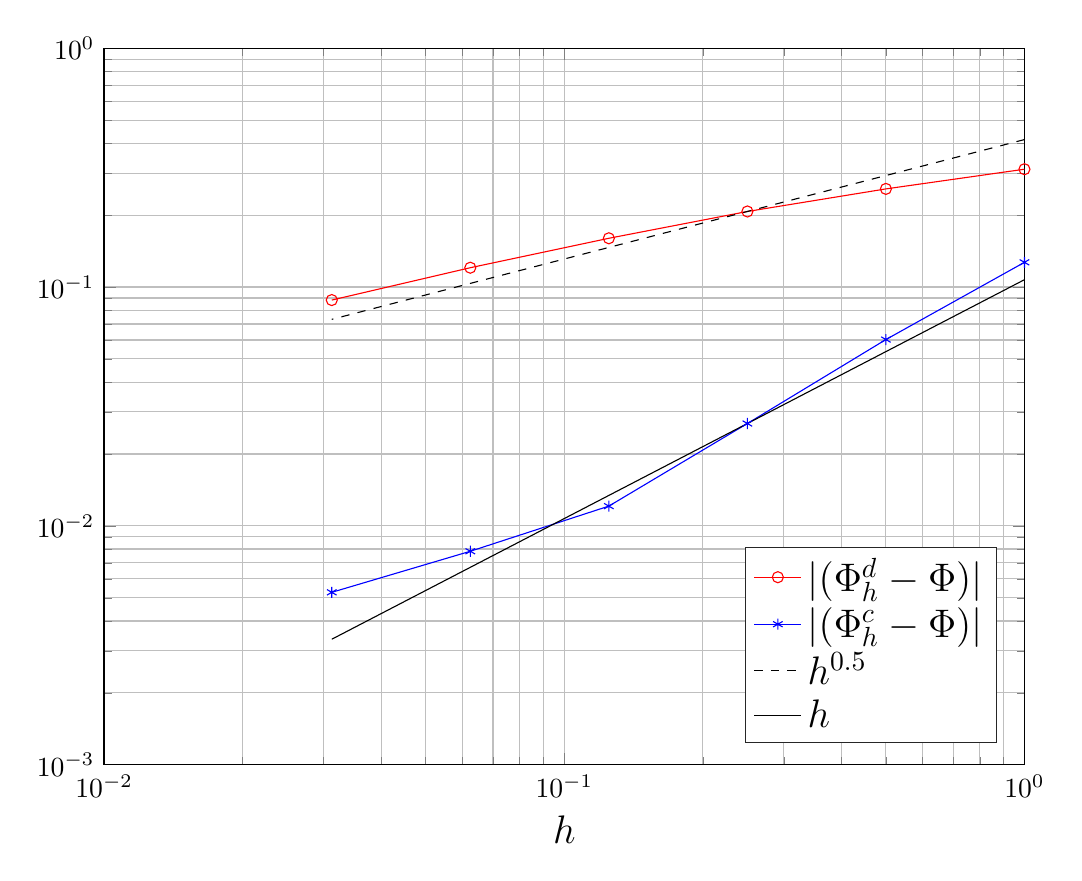
\begin{tikzpicture}

\begin{axis}[%
width=4.602in,
height=3.583in,
at={(0.772in,0.484in)},
scale only axis,
xmode=log,
xmin=0.01,
xmax=1,
xminorticks=true,
xlabel={$h$},
xlabel style={font=\Large},
xmajorgrids,
xminorgrids,
ymode=log,
ymin=0.001,
ymax=1,
yminorticks=true,
ymajorgrids,
yminorgrids,
axis background/.style={fill=white},
legend pos = south east,
legend style={legend cell align=left,align=left,draw=white!15!black,font=\Large}
]
\addplot [color=red,solid,mark=o,mark options={solid}]
  table[row sep=crcr]{%
1	0.31134162505938\\
0.5	0.25753162505938\\
0.25	0.20716162505938\\
0.125	0.15999162505938\\
0.0625	0.12047162505938\\
0.03125	0.0881916250593803\\
};
\addlegendentry{$|\E(\Phi_h^d - \Phi)|$};

\addplot [color=blue,solid,mark=asterisk,mark options={solid}]
  table[row sep=crcr]{%
1	0.12689162505938\\
0.5	0.0602816250593803\\
0.25	0.0268316250593803\\
0.125	0.0121016250593803\\
0.0625	0.00783162505938029\\
0.03125	0.00527162505938028\\
};
\addlegendentry{$|\E(\Phi_h^c - \Phi)|$};

\addplot [color=black,dashed]
  table[row sep=crcr]{%
1	0.41432325011876\\
0.5	0.292970779762226\\
0.25	0.20716162505938\\
0.125	0.146485389881113\\
0.0625	0.10358081252969\\
0.03125	0.0732426949405564\\
};
\addlegendentry{$h^{0.5}$};

\addplot [color=black,solid]
  table[row sep=crcr]{%
1	0.107326500237521\\
0.5	0.0536632501187606\\
0.25	0.0268316250593803\\
0.125	0.0134158125296902\\
0.0625	0.00670790626484508\\
0.03125	0.00335395313242254\\
};
\addlegendentry{$h$};

\end{axis}
\end{tikzpicture}%
 }  
        \caption{Convergence of CEM and DEM.}
        \label{fig:ReflTwoDPhi}
    \end{subfigure}
    \begin{subfigure}{0.49\linewidth}
        \centering
        \resizebox{1\linewidth}{!}{% This file was created by matlab2tikz.
%
%The latest updates can be retrieved from
%  http://www.mathworks.com/matlabcentral/fileexchange/22022-matlab2tikz-matlab2tikz
%where you can also make suggestions and rate matlab2tikz.
%
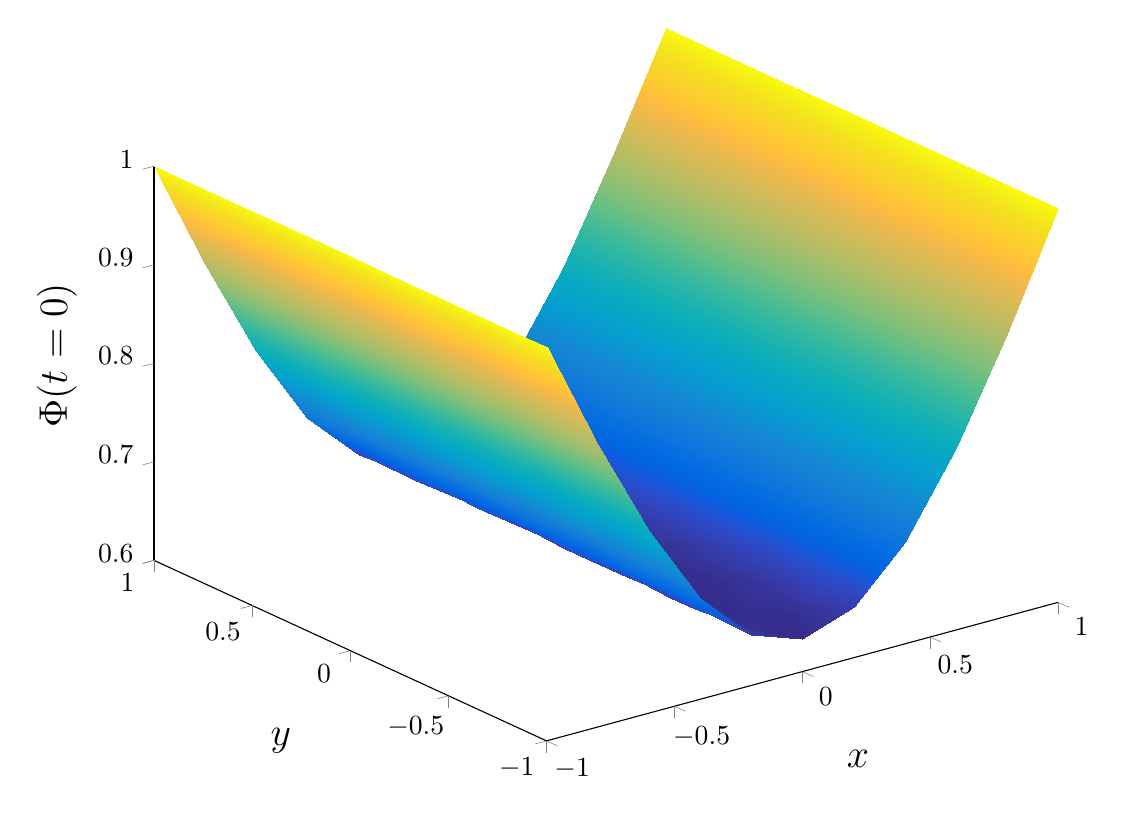
\begin{tikzpicture}

\begin{axis}[%
width=4.521in,
height=3.566in,
at={(0.758in,0.481in)},
scale only axis,
colormap={mymap}{[1pt] rgb(0pt)=(0.2081,0.1663,0.5292); rgb(1pt)=(0.211624,0.189781,0.577676); rgb(2pt)=(0.212252,0.213771,0.626971); rgb(3pt)=(0.2081,0.2386,0.677086); rgb(4pt)=(0.195905,0.264457,0.7279); rgb(5pt)=(0.170729,0.291938,0.779248); rgb(6pt)=(0.125271,0.324243,0.830271); rgb(7pt)=(0.0591333,0.359833,0.868333); rgb(8pt)=(0.0116952,0.38751,0.881957); rgb(9pt)=(0.00595714,0.408614,0.882843); rgb(10pt)=(0.0165143,0.4266,0.878633); rgb(11pt)=(0.0328524,0.443043,0.871957); rgb(12pt)=(0.0498143,0.458571,0.864057); rgb(13pt)=(0.0629333,0.47369,0.855438); rgb(14pt)=(0.0722667,0.488667,0.8467); rgb(15pt)=(0.0779429,0.503986,0.838371); rgb(16pt)=(0.0793476,0.520024,0.831181); rgb(17pt)=(0.0749429,0.537543,0.826271); rgb(18pt)=(0.0640571,0.556986,0.823957); rgb(19pt)=(0.0487714,0.577224,0.822829); rgb(20pt)=(0.0343429,0.596581,0.819852); rgb(21pt)=(0.0265,0.6137,0.8135); rgb(22pt)=(0.0238905,0.628662,0.803762); rgb(23pt)=(0.0230905,0.641786,0.791267); rgb(24pt)=(0.0227714,0.653486,0.776757); rgb(25pt)=(0.0266619,0.664195,0.760719); rgb(26pt)=(0.0383714,0.674271,0.743552); rgb(27pt)=(0.0589714,0.683757,0.725386); rgb(28pt)=(0.0843,0.692833,0.706167); rgb(29pt)=(0.113295,0.7015,0.685857); rgb(30pt)=(0.145271,0.709757,0.664629); rgb(31pt)=(0.180133,0.717657,0.642433); rgb(32pt)=(0.217829,0.725043,0.619262); rgb(33pt)=(0.258643,0.731714,0.595429); rgb(34pt)=(0.302171,0.737605,0.571186); rgb(35pt)=(0.348167,0.742433,0.547267); rgb(36pt)=(0.395257,0.7459,0.524443); rgb(37pt)=(0.44201,0.748081,0.503314); rgb(38pt)=(0.487124,0.749062,0.483976); rgb(39pt)=(0.530029,0.749114,0.466114); rgb(40pt)=(0.570857,0.748519,0.44939); rgb(41pt)=(0.609852,0.747314,0.433686); rgb(42pt)=(0.6473,0.7456,0.4188); rgb(43pt)=(0.683419,0.743476,0.404433); rgb(44pt)=(0.71841,0.741133,0.390476); rgb(45pt)=(0.752486,0.7384,0.376814); rgb(46pt)=(0.785843,0.735567,0.363271); rgb(47pt)=(0.818505,0.732733,0.34979); rgb(48pt)=(0.850657,0.7299,0.336029); rgb(49pt)=(0.882433,0.727433,0.3217); rgb(50pt)=(0.913933,0.725786,0.306276); rgb(51pt)=(0.944957,0.726114,0.288643); rgb(52pt)=(0.973895,0.731395,0.266648); rgb(53pt)=(0.993771,0.745457,0.240348); rgb(54pt)=(0.999043,0.765314,0.216414); rgb(55pt)=(0.995533,0.786057,0.196652); rgb(56pt)=(0.988,0.8066,0.179367); rgb(57pt)=(0.978857,0.827143,0.163314); rgb(58pt)=(0.9697,0.848138,0.147452); rgb(59pt)=(0.962586,0.870514,0.1309); rgb(60pt)=(0.958871,0.8949,0.113243); rgb(61pt)=(0.959824,0.921833,0.0948381); rgb(62pt)=(0.9661,0.951443,0.0755333); rgb(63pt)=(0.9763,0.9831,0.0538)},
xmin=-1,
xmax=1,
tick align=outside,
xlabel={$x$},
xlabel style={font=\Large},
ymin=-1,
ymax=1,
ylabel={$y$},
ylabel style={font=\Large},
zmin=0.6,
zmax=1,
zlabel={$\Phi\text{(t=0)}$},
zlabel style={font=\Large},
view={-37.5}{30},
axis background/.style={fill=white},
axis x line*=bottom,
axis y line*=left,
axis z line*=left
]

\addplot3[area legend,solid,table/row sep=crcr,patch,shader=interp,forget plot,patch table={%
0	1	2\\
3	4	5\\
6	7	8\\
9	10	11\\
12	13	14\\
15	16	17\\
18	19	20\\
21	22	23\\
24	25	26\\
27	28	29\\
30	31	32\\
33	34	35\\
36	37	38\\
39	40	41\\
42	43	44\\
45	46	47\\
48	49	50\\
51	52	53\\
54	55	56\\
57	58	59\\
60	61	62\\
63	64	65\\
66	67	68\\
69	70	71\\
72	73	74\\
75	76	77\\
78	79	80\\
81	82	83\\
84	85	86\\
87	88	89\\
90	91	92\\
93	94	95\\
96	97	98\\
99	100	101\\
102	103	104\\
105	106	107\\
108	109	110\\
111	112	113\\
114	115	116\\
117	118	119\\
120	121	122\\
123	124	125\\
126	127	128\\
129	130	131\\
132	133	134\\
135	136	137\\
138	139	140\\
141	142	143\\
144	145	146\\
147	148	149\\
150	151	152\\
153	154	155\\
156	157	158\\
159	160	161\\
162	163	164\\
165	166	167\\
168	169	170\\
171	172	173\\
174	175	176\\
177	178	179\\
180	181	182\\
183	184	185\\
186	187	188\\
189	190	191\\
192	193	194\\
195	196	197\\
198	199	200\\
201	202	203\\
204	205	206\\
207	208	209\\
210	211	212\\
213	214	215\\
216	217	218\\
219	220	221\\
222	223	224\\
225	226	227\\
228	229	230\\
231	232	233\\
234	235	236\\
237	238	239\\
240	241	242\\
243	244	245\\
246	247	248\\
249	250	251\\
252	253	254\\
255	256	257\\
258	259	260\\
261	262	263\\
264	265	266\\
267	268	269\\
270	271	272\\
273	274	275\\
276	277	278\\
279	280	281\\
282	283	284\\
285	286	287\\
288	289	290\\
291	292	293\\
294	295	296\\
297	298	299\\
300	301	302\\
303	304	305\\
306	307	308\\
309	310	311\\
312	313	314\\
315	316	317\\
318	319	320\\
321	322	323\\
324	325	326\\
327	328	329\\
330	331	332\\
333	334	335\\
336	337	338\\
339	340	341\\
342	343	344\\
345	346	347\\
348	349	350\\
351	352	353\\
354	355	356\\
357	358	359\\
360	361	362\\
363	364	365\\
366	367	368\\
369	370	371\\
372	373	374\\
375	376	377\\
378	379	380\\
381	382	383\\
384	385	386\\
387	388	389\\
390	391	392\\
393	394	395\\
396	397	398\\
399	400	401\\
402	403	404\\
405	406	407\\
408	409	410\\
411	412	413\\
414	415	416\\
417	418	419\\
420	421	422\\
423	424	425\\
426	427	428\\
429	430	431\\
432	433	434\\
435	436	437\\
438	439	440\\
441	442	443\\
444	445	446\\
447	448	449\\
450	451	452\\
453	454	455\\
456	457	458\\
459	460	461\\
462	463	464\\
465	466	467\\
468	469	470\\
471	472	473\\
474	475	476\\
477	478	479\\
480	481	482\\
483	484	485\\
486	487	488\\
489	490	491\\
492	493	494\\
495	496	497\\
498	499	500\\
501	502	503\\
504	505	506\\
507	508	509\\
510	511	512\\
513	514	515\\
516	517	518\\
519	520	521\\
522	523	524\\
525	526	527\\
528	529	530\\
531	532	533\\
534	535	536\\
537	538	539\\
540	541	542\\
543	544	545\\
546	547	548\\
549	550	551\\
552	553	554\\
555	556	557\\
558	559	560\\
561	562	563\\
564	565	566\\
567	568	569\\
570	571	572\\
573	574	575\\
576	577	578\\
579	580	581\\
582	583	584\\
585	586	587\\
588	589	590\\
591	592	593\\
594	595	596\\
597	598	599\\
600	601	602\\
603	604	605\\
606	607	608\\
609	610	611\\
612	613	614\\
615	616	617\\
618	619	620\\
621	622	623\\
624	625	626\\
627	628	629\\
630	631	632\\
633	634	635\\
636	637	638\\
639	640	641\\
642	643	644\\
645	646	647\\
648	649	650\\
651	652	653\\
654	655	656\\
657	658	659\\
660	661	662\\
663	664	665\\
666	667	668\\
669	670	671\\
672	673	674\\
675	676	677\\
678	679	680\\
681	682	683\\
684	685	686\\
687	688	689\\
690	691	692\\
693	694	695\\
696	697	698\\
699	700	701\\
702	703	704\\
705	706	707\\
708	709	710\\
711	712	713\\
714	715	716\\
717	718	719\\
720	721	722\\
723	724	725\\
726	727	728\\
729	730	731\\
732	733	734\\
735	736	737\\
738	739	740\\
741	742	743\\
744	745	746\\
747	748	749\\
750	751	752\\
753	754	755\\
756	757	758\\
759	760	761\\
762	763	764\\
765	766	767\\
768	769	770\\
771	772	773\\
774	775	776\\
777	778	779\\
780	781	782\\
783	784	785\\
786	787	788\\
789	790	791\\
792	793	794\\
795	796	797\\
798	799	800\\
801	802	803\\
804	805	806\\
807	808	809\\
810	811	812\\
813	814	815\\
816	817	818\\
819	820	821\\
822	823	824\\
825	826	827\\
828	829	830\\
831	832	833\\
834	835	836\\
837	838	839\\
840	841	842\\
843	844	845\\
846	847	848\\
849	850	851\\
852	853	854\\
855	856	857\\
858	859	860\\
861	862	863\\
864	865	866\\
867	868	869\\
870	871	872\\
873	874	875\\
876	877	878\\
879	880	881\\
882	883	884\\
885	886	887\\
888	889	890\\
891	892	893\\
894	895	896\\
897	898	899\\
900	901	902\\
903	904	905\\
906	907	908\\
909	910	911\\
912	913	914\\
915	916	917\\
918	919	920\\
921	922	923\\
924	925	926\\
927	928	929\\
930	931	932\\
933	934	935\\
}]
table[row sep=crcr, point meta=\thisrow{c}] {%
x	y	z	c\\
-0.8	1	0.886661502769369	0.886661502769369\\
-1	1	1	1\\
-0.870979864217162	0.874090623781756	0.926371924403184	0.926371924403184\\
-0.6	1	0.784485328696294	0.784485328696294\\
-0.8	1	0.886661502769369	0.886661502769369\\
-0.715759069893515	0.851783447512538	0.84196267634871	0.84196267634871\\
-0.4	1	0.702781277702834	0.702781277702834\\
-0.6	1	0.784485328696294	0.784485328696294\\
-0.553557227232278	0.85599352174284	0.763831325159682	0.763831325159682\\
-0.2	1	0.650629573483716	0.650629573483716\\
-0.4	1	0.702781277702834	0.702781277702834\\
-0.256371139537587	0.844436132195903	0.662879593141817	0.662879593141817\\
0	1	0.632136025890254	0.632136025890254\\
-0.2	1	0.650629573483716	0.650629573483716\\
-0.123171927132804	0.882407229449651	0.640563409449267	0.640563409449267\\
0.2	1	0.650784455386188	0.650784455386188\\
0	1	0.632136025890254	0.632136025890254\\
0.138576080047019	0.836444863570092	0.641885576816903	0.641885576816903\\
0.4	1	0.703168980579003	0.703168980579003\\
0.2	1	0.650784455386188	0.650784455386188\\
0.314746867281053	0.841650113118016	0.677236387434948	0.677236387434948\\
0.6	1	0.78448205009674	0.78448205009674\\
0.4	1	0.703168980579003	0.703168980579003\\
0.500557557249754	0.834821560479383	0.741120831557631	0.741120831557631\\
1	0.8	1	1\\
1	1	1	1\\
0.913245437763783	0.903908655259532	0.950362685209763	0.950362685209763\\
0.8	1	0.88657405843758	0.88657405843758\\
0.6	1	0.78448205009674	0.78448205009674\\
0.6908636124721	0.827426566529025	0.829083787417288	0.829083787417288\\
1	1	1	1\\
0.8	1	0.88657405843758	0.88657405843758\\
0.913245437763783	0.903908655259532	0.950362685209763	0.950362685209763\\
0.913245437763783	0.903908655259532	0.950362685209763	0.950362685209763\\
0.8	1	0.88657405843758	0.88657405843758\\
0.853111865010539	0.81689479082676	0.916326946586619	0.916326946586619\\
1	0.6	1	1\\
1	0.8	1	1\\
0.913257156072776	0.71766207885242	0.950402731824633	0.950402731824633\\
1	0.4	1	1\\
1	0.6	1	1\\
0.858172452446661	0.489687445107711	0.919175927460463	0.919175927460463\\
1	0.2	1	1\\
1	0.4	1	1\\
0.801876020058965	0.306586241275605	0.887604311618317	0.887604311618317\\
1	-0.2	1	1\\
1	0	1	1\\
0.842830738889788	-0.109162193087545	0.910650575746641	0.910650575746641\\
1	-0.4	1	1\\
1	-0.2	1	1\\
0.839553137409186	-0.294644298019888	0.908694258634168	0.908694258634168\\
1	-0.6	1	1\\
1	-0.4	1	1\\
0.825961266928206	-0.490102064147121	0.900920385850852	0.900920385850852\\
0.8	-1	0.886482880444004	0.886482880444004\\
1	-1	1	1\\
0.903543131650638	-0.913183857559471	0.944951211463095	0.944951211463095\\
1	-0.8	1	1\\
1	-0.6	1	1\\
0.822757598423982	-0.688930059869196	0.899162246555509	0.899162246555509\\
1	-1	1	1\\
1	-0.8	1	1\\
0.903543131650638	-0.913183857559471	0.944951211463095	0.944951211463095\\
0.903543131650638	-0.913183857559471	0.944951211463095	0.944951211463095\\
1	-0.8	1	1\\
0.815246907920555	-0.852962033044177	0.895288501641487	0.895288501641487\\
0.6	-1	0.784296457589665	0.784296457589665\\
0.8	-1	0.886482880444004	0.886482880444004\\
0.716262971529556	-0.913440138799354	0.842529925902384	0.842529925902384\\
0.4	-1	0.703111509399902	0.703111509399902\\
0.6	-1	0.784296457589665	0.784296457589665\\
0.486610676987292	-0.860815662729556	0.735606241744598	0.735606241744598\\
0.2	-1	0.65107448085574	0.65107448085574\\
0.4	-1	0.703111509399902	0.703111509399902\\
0.30415666992098	-0.806486553345674	0.673626853358672	0.673626853358672\\
-0.2	-1	0.650803162223099	0.650803162223099\\
0	-1	0.632867110284715	0.632867110284715\\
-0.108836774839956	-0.842631178463089	0.638332217570717	0.638332217570717\\
-0.4	-1	0.703204587981096	0.703204587981096\\
-0.2	-1	0.650803162223099	0.650803162223099\\
-0.295155054484333	-0.839202734226978	0.671924116854502	0.671924116854502\\
-0.6	-1	0.784417631343421	0.784417631343421\\
-0.4	-1	0.703204587981096	0.703204587981096\\
-0.491181950150036	-0.827450133500077	0.737178341272982	0.737178341272982\\
-1	-0.8	1	1\\
-1	-1	1	1\\
-0.913179600822541	-0.903978796898105	0.950282014739715	0.950282014739715\\
-0.8	-1	0.886486216639573	0.886486216639573\\
-0.6	-1	0.784417631343421	0.784417631343421\\
-0.689383148912005	-0.825669061227738	0.828153670218637	0.828153670218637\\
-1	-1	1	1\\
-0.8	-1	0.886486216639573	0.886486216639573\\
-0.913179600822541	-0.903978796898105	0.950282014739715	0.950282014739715\\
-0.913179600822541	-0.903978796898105	0.950282014739715	0.950282014739715\\
-0.8	-1	0.886486216639573	0.886486216639573\\
-0.852930471573381	-0.817084814175369	0.916144797873899	0.916144797873899\\
-1	-0.6	1	1\\
-1	-0.8	1	1\\
-0.913349182557632	-0.71824277938499	0.950410379967385	0.950410379967385\\
-1	-0.4	1	1\\
-1	-0.6	1	1\\
-0.858612569930114	-0.502582179815703	0.919413375191812	0.919413375191812\\
-1	-0.2	1	1\\
-1	-0.4	1	1\\
-0.875147249859378	-0.2495178793164	0.928707588314099	0.928707588314099\\
0.822757598423982	-0.688930059869196	0.899162246555509	0.899162246555509\\
1	-0.6	1	1\\
0.825961266928206	-0.490102064147121	0.900920385850852	0.900920385850852\\
-1	0.2	1	1\\
-1	0	1	1\\
-0.878430687062504	0.0687937548368703	0.930704277937362	0.930704277937362\\
-1	0.4	1	1\\
-1	0.2	1	1\\
-0.858638192546528	0.336283758462884	0.919489028593257	0.919489028593257\\
0.314746867281053	0.841650113118016	0.677236387434948	0.677236387434948\\
0.2	1	0.650784455386188	0.650784455386188\\
0.138576080047019	0.836444863570092	0.641885576816903	0.641885576816903\\
-1	0.6	1	1\\
-1	0.4	1	1\\
-0.81542002432126	0.514265339146589	0.895152687835795	0.895152687835795\\
-1	0	1	1\\
-1	-0.2	1	1\\
-0.849550627410001	-0.0857161204413969	0.914194574024607	0.914194574024607\\
-0.81542002432126	0.514265339146589	0.895152687835795	0.895152687835795\\
-1	0.4	1	1\\
-0.858638192546528	0.336283758462884	0.919489028593257	0.919489028593257\\
0	-1	0.632867110284715	0.632867110284715\\
0.2	-1	0.65107448085574	0.65107448085574\\
0.0842448278397462	-0.826656651009239	0.63604755415419	0.63604755415419\\
-0.295155054484333	-0.839202734226978	0.671924116854502	0.671924116854502\\
-0.2	-1	0.650803162223099	0.650803162223099\\
-0.108836774839956	-0.842631178463089	0.638332217570717	0.638332217570717\\
1	0	1	1\\
1	0.2	1	1\\
0.825000730866433	0.0840636812185947	0.900569694652281	0.900569694652281\\
0.839553137409186	-0.294644298019888	0.908694258634168	0.908694258634168\\
1	-0.2	1	1\\
0.842830738889788	-0.109162193087545	0.910650575746641	0.910650575746641\\
-0.421476522111469	0.76529746608585	0.710789563255218	0.710789563255218\\
-0.4	1	0.702781277702834	0.702781277702834\\
-0.553557227232278	0.85599352174284	0.763831325159682	0.763831325159682\\
-1	1	1	1\\
-1	0.8	1	1\\
-0.870979864217162	0.874090623781756	0.926371924403184	0.926371924403184\\
-1	0.8	1	1\\
-1	0.6	1	1\\
-0.838909094432717	0.717165597536304	0.908109180949002	0.908109180949002\\
-0.870979864217162	0.874090623781756	0.926371924403184	0.926371924403184\\
-1	0.8	1	1\\
-0.838909094432717	0.717165597536304	0.908109180949002	0.908109180949002\\
-0.689383148912005	-0.825669061227738	0.828153670218637	0.828153670218637\\
-0.6	-1	0.784417631343421	0.784417631343421\\
-0.491181950150036	-0.827450133500077	0.737178341272982	0.737178341272982\\
0.162899107774523	0.0782930267751429	0.645059759299502	0.645059759299502\\
-0.0145232187187818	0.0259493451768655	0.633718540987385	0.633718540987385\\
0.0995954131227801	-0.0711056079718885	0.638519798904632	0.638519798904632\\
0.6908636124721	0.827426566529025	0.829083787417288	0.829083787417288\\
0.6	1	0.78448205009674	0.78448205009674\\
0.500557557249754	0.834821560479383	0.741120831557631	0.741120831557631\\
-0.0437189086592884	-0.1794562797288	0.633632589259963	0.633632589259963\\
-0.0145232187187818	0.0259493451768655	0.633718540987385	0.633718540987385\\
-0.183666461200581	-0.0196981175980336	0.64858714731975	0.64858714731975\\
-0.183666461200581	-0.0196981175980336	0.64858714731975	0.64858714731975\\
-0.0145232187187818	0.0259493451768655	0.633718540987385	0.633718540987385\\
-0.143244730260345	0.15312684048721	0.642715109320877	0.642715109320877\\
-0.573742666641828	0.478792000601255	0.772980006673901	0.772980006673901\\
-0.435775856529045	0.402580883145608	0.71656862984604	0.71656862984604\\
-0.436448993108287	0.574739898722634	0.716346127137646	0.716346127137646\\
-0.777645420963466	0.191713474052978	0.874448623162011	0.874448623162011\\
-1	0.2	1	1\\
-0.878430687062504	0.0687937548368703	0.930704277937362	0.930704277937362\\
-0.308985524220196	-0.434191396690207	0.675725952222081	0.675725952222081\\
-0.44256229481138	-0.30475784338953	0.719056444957801	0.719056444957801\\
-0.504626867096141	-0.476494146294975	0.742748657802048	0.742748657802048\\
0.30415666992098	-0.806486553345674	0.673626853358672	0.673626853358672\\
0.4	-1	0.703111509399902	0.703111509399902\\
0.486610676987292	-0.860815662729556	0.735606241744598	0.735606241744598\\
0.0893690793198263	-0.463478876426208	0.637096459558783	0.637096459558783\\
0.261928641455601	-0.488055957894452	0.663932632345156	0.663932632345156\\
0.2060410026947	-0.342035240885369	0.653019979296508	0.653019979296508\\
0.801876020058965	0.306586241275605	0.887604311618317	0.887604311618317\\
1	0.4	1	1\\
0.858172452446661	0.489687445107711	0.919175927460463	0.919175927460463\\
0.500557557249754	0.834821560479383	0.741120831557631	0.741120831557631\\
0.4	1	0.703168980579003	0.703168980579003\\
0.314746867281053	0.841650113118016	0.677236387434948	0.677236387434948\\
-0.0174658545926647	0.801898927302032	0.634008791412185	0.634008791412185\\
0	1	0.632136025890254	0.632136025890254\\
-0.123171927132804	0.882407229449651	0.640563409449267	0.640563409449267\\
0.629591208237007	0.150059132096618	0.798255023549285	0.798255023549285\\
0.464005364535939	0.260203010616371	0.726738167526826	0.726738167526826\\
0.457941066948159	0.074681360252563	0.724409350972182	0.724409350972182\\
-0.536183382478912	-0.125067364855863	0.755757598127736	0.755757598127736\\
-0.44256229481138	-0.30475784338953	0.719056444957801	0.719056444957801\\
-0.376489904228021	-0.187383275146088	0.696362240014	0.696362240014\\
0.825961266928206	-0.490102064147121	0.900920385850852	0.900920385850852\\
1	-0.4	1	1\\
0.839553137409186	-0.294644298019888	0.908694258634168	0.908694258634168\\
-0.491181950150036	-0.827450133500077	0.737178341272982	0.737178341272982\\
-0.4	-1	0.703204587981096	0.703204587981096\\
-0.295155054484333	-0.839202734226978	0.671924116854502	0.671924116854502\\
0.151932036409303	-0.636460365815934	0.643692805956064	0.643692805956064\\
0.261928641455601	-0.488055957894452	0.663932632345156	0.663932632345156\\
0.0893690793198263	-0.463478876426208	0.637096459558783	0.637096459558783\\
-0.31111533158028	-0.281732042536466	0.67724909146464	0.67724909146464\\
-0.241660277500026	-0.172513969577467	0.659692388466087	0.659692388466087\\
-0.376489904228021	-0.187383275146088	0.696362240014	0.696362240014\\
-0.796122724389227	-0.361886425045465	0.884582357533658	0.884582357533658\\
-0.695084883753552	-0.495926997595022	0.831190603055093	0.831190603055093\\
-0.617615903555302	-0.32670910304294	0.793129540476502	0.793129540476502\\
0.321736948673632	-0.218404805181936	0.679231673171288	0.679231673171288\\
0.149400916774043	-0.200302697508326	0.643315704349224	0.643315704349224\\
0.2060410026947	-0.342035240885369	0.653019979296508	0.653019979296508\\
0.459725917575231	0.478817132146761	0.724537831702122	0.724537831702122\\
0.464005364535939	0.260203010616371	0.726738167526826	0.726738167526826\\
0.609248416595618	0.336700564235885	0.789294480401005	0.789294480401005\\
-0.591992818593216	-0.654470500305776	0.78055052322873	0.78055052322873\\
-0.368952164395011	-0.646051178924541	0.692833679100329	0.692833679100329\\
-0.504626867096141	-0.476494146294975	0.742748657802048	0.742748657802048\\
0.646526572158138	-0.5892372548303	0.806693817934909	0.806693817934909\\
0.647783933105589	-0.365727428795828	0.8070755170843	0.8070755170843\\
0.453484147433517	-0.490455219207141	0.721994331149971	0.721994331149971\\
-0.8	1	0.886661502769369	0.886661502769369\\
-0.870979864217162	0.874090623781756	0.926371924403184	0.926371924403184\\
-0.715759069893515	0.851783447512538	0.84196267634871	0.84196267634871\\
-0.436448993108287	0.574739898722634	0.716346127137646	0.716346127137646\\
-0.435775856529045	0.402580883145608	0.71656862984604	0.71656862984604\\
-0.305196827885855	0.481941510996423	0.675471802226354	0.675471802226354\\
0.651531723544283	-0.800304145152872	0.809208076605386	0.809208076605386\\
0.6	-1	0.784296457589665	0.784296457589665\\
0.716262971529556	-0.913440138799354	0.842529925902384	0.842529925902384\\
0.651531723544283	-0.800304145152872	0.809208076605386	0.809208076605386\\
0.822757598423982	-0.688930059869196	0.899162246555509	0.899162246555509\\
0.646526572158138	-0.5892372548303	0.806693817934909	0.806693817934909\\
0.457941066948159	0.074681360252563	0.724409350972182	0.724409350972182\\
0.464005364535939	0.260203010616371	0.726738167526826	0.726738167526826\\
0.313359205867812	0.176240487473655	0.676715887699215	0.676715887699215\\
0.799426193403826	0.656174087711846	0.886260631781478	0.886260631781478\\
1	0.6	1	1\\
0.913257156072776	0.71766207885242	0.950402731824633	0.950402731824633\\
-0.800381152695487	-0.658205081403852	0.886688421144949	0.886688421144949\\
-1	-0.6	1	1\\
-0.913349182557632	-0.71824277938499	0.950410379967385	0.950410379967385\\
-0.800381152695487	-0.658205081403852	0.886688421144949	0.886688421144949\\
-0.689383148912005	-0.825669061227738	0.828153670218637	0.828153670218637\\
-0.591992818593216	-0.654470500305776	0.78055052322873	0.78055052322873\\
-0.131538906378604	0.468005506270669	0.640754428869951	0.640754428869951\\
0.0468419620052357	0.523978954343319	0.634387932516724	0.634387932516724\\
-0.0677763280124889	0.648507972991784	0.635453761471089	0.635453761471089\\
0.172508063347201	0.422930104621211	0.646971834078828	0.646971834078828\\
0.0468419620052357	0.523978954343319	0.634387932516724	0.634387932516724\\
0.0285171270359044	0.362157622648837	0.633906337560461	0.633906337560461\\
0.453484147433517	-0.490455219207141	0.721994331149971	0.721994331149971\\
0.261928641455601	-0.488055957894452	0.663932632345156	0.663932632345156\\
0.32991065048365	-0.623943472007708	0.681939815211704	0.681939815211704\\
0.0893690793198263	-0.463478876426208	0.637096459558783	0.637096459558783\\
-0.0468923144628943	-0.37201189317892	0.635212674981464	0.635212674981464\\
-0.0519572972000214	-0.516668038614571	0.635383314295437	0.635383314295437\\
0.801876020058965	0.306586241275605	0.887604311618317	0.887604311618317\\
0.687082418720278	0.487393175878324	0.826967797902895	0.826967797902895\\
0.609248416595618	0.336700564235885	0.789294480401005	0.789294480401005\\
0.457941066948159	0.074681360252563	0.724409350972182	0.724409350972182\\
0.386220146013541	-0.0691483215457924	0.699337607275974	0.699337607275974\\
0.521855887175084	-0.0613271652026621	0.750290590365668	0.750290590365668\\
0.0893728715906334	0.678554065055819	0.637164086828247	0.637164086828247\\
0.0468419620052357	0.523978954343319	0.634387932516724	0.634387932516724\\
0.193142943255321	0.563632036809665	0.65047130858186	0.65047130858186\\
-0.467792458521678	0.219937427890346	0.727668371205196	0.727668371205196\\
-0.435775856529045	0.402580883145608	0.71656862984604	0.71656862984604\\
-0.560240270361451	0.344844062180542	0.766988939272872	0.766988939272872\\
0.0172621493060368	0.196448852647962	0.633713314361824	0.633713314361824\\
0.167453556422288	0.263155683226473	0.64603950792469	0.64603950792469\\
0.0285171270359044	0.362157622648837	0.633906337560461	0.633906337560461\\
-0.777645420963466	0.191713474052978	0.874448623162011	0.874448623162011\\
-0.617913717697813	0.079971000861777	0.792955541583216	0.792955541583216\\
-0.624616411644707	0.242665578371416	0.796542846610872	0.796542846610872\\
-0.536183382478912	-0.125067364855863	0.755757598127736	0.755757598127736\\
-0.617913717697813	0.079971000861777	0.792955541583216	0.792955541583216\\
-0.699519166874299	-0.0584145433376073	0.833664955062639	0.833664955062639\\
-0.421476522111469	0.76529746608585	0.710789563255218	0.710789563255218\\
-0.629666025324687	0.659481894250005	0.797657769267581	0.797657769267581\\
-0.436448993108287	0.574739898722634	0.716346127137646	0.716346127137646\\
-0.467792458521678	0.219937427890346	0.727668371205196	0.727668371205196\\
-0.617913717697813	0.079971000861777	0.792955541583216	0.792955541583216\\
-0.456541297467842	0.0462574378515442	0.724331567787662	0.724331567787662\\
-0.796122724389227	-0.361886425045465	0.884582357533658	0.884582357533658\\
-1	-0.4	1	1\\
-0.858612569930114	-0.502582179815703	0.919413375191812	0.919413375191812\\
0.30415666992098	-0.806486553345674	0.673626853358672	0.673626853358672\\
0.478214140797659	-0.695585476223675	0.731941724196132	0.731941724196132\\
0.32991065048365	-0.623943472007708	0.681939815211704	0.681939815211704\\
-0.350427977113875	-0.0568798710953585	0.687527845399035	0.687527845399035\\
-0.241660277500026	-0.172513969577467	0.659692388466087	0.659692388466087\\
-0.183666461200581	-0.0196981175980336	0.64858714731975	0.64858714731975\\
0.521855887175084	-0.0613271652026621	0.750290590365668	0.750290590365668\\
0.386220146013541	-0.0691483215457924	0.699337607275974	0.699337607275974\\
0.456651668322266	-0.168447833276863	0.724472173228028	0.724472173228028\\
-0.256371139537587	0.844436132195903	0.662879593141817	0.662879593141817\\
-0.251840934393812	0.65073582839654	0.661191483037017	0.661191483037017\\
-0.14310781983293	0.765817634248709	0.643111778521292	0.643111778521292\\
1	0.8	1	1\\
0.913245437763783	0.903908655259532	0.950362685209763	0.950362685209763\\
0.853111865010539	0.81689479082676	0.916326946586619	0.916326946586619\\
-0.131538906378604	0.468005506270669	0.640754428869951	0.640754428869951\\
-0.0999792356165469	0.29750658388758	0.638572579319181	0.638572579319181\\
0.0285171270359044	0.362157622648837	0.633906337560461	0.633906337560461\\
0.799426193403826	0.656174087711846	0.886260631781478	0.886260631781478\\
0.687082418720278	0.487393175878324	0.826967797902895	0.826967797902895\\
0.858172452446661	0.489687445107711	0.919175927460463	0.919175927460463\\
0.239679041234336	-0.0747988778282174	0.659571694557361	0.659571694557361\\
0.386220146013541	-0.0691483215457924	0.699337607275974	0.699337607275974\\
0.312829618686655	0.0361464359017708	0.677332550335988	0.677332550335988\\
0.651531723544283	-0.800304145152872	0.809208076605386	0.809208076605386\\
0.478214140797659	-0.695585476223675	0.731941724196132	0.731941724196132\\
0.486610676987292	-0.860815662729556	0.735606241744598	0.735606241744598\\
-0.0437189086592884	-0.1794562797288	0.633632589259963	0.633632589259963\\
-0.0468923144628943	-0.37201189317892	0.635212674981464	0.635212674981464\\
0.0706839927525276	-0.312287735493971	0.636585029966717	0.636585029966717\\
-0.617615903555302	-0.32670910304294	0.793129540476502	0.793129540476502\\
-0.695084883753552	-0.495926997595022	0.831190603055093	0.831190603055093\\
-0.504626867096141	-0.476494146294975	0.742748657802048	0.742748657802048\\
-0.308985524220196	-0.434191396690207	0.675725952222081	0.675725952222081\\
-0.368952164395011	-0.646051178924541	0.692833679100329	0.692833679100329\\
-0.188699779816531	-0.572089273359516	0.64914787186478	0.64914787186478\\
0.467892646677106	-0.300972929247376	0.728351764655454	0.728351764655454\\
0.647783933105589	-0.365727428795828	0.8070755170843	0.8070755170843\\
0.581538749766835	-0.190353470678335	0.7766731281901	0.7766731281901\\
0.321736948673632	-0.218404805181936	0.679231673171288	0.679231673171288\\
0.386220146013541	-0.0691483215457924	0.699337607275974	0.699337607275974\\
0.239679041234336	-0.0747988778282174	0.659571694557361	0.659571694557361\\
0.6908636124721	0.827426566529025	0.829083787417288	0.829083787417288\\
0.500557557249754	0.834821560479383	0.741120831557631	0.741120831557631\\
0.590963022235164	0.660549521945042	0.78045897621863	0.78045897621863\\
0.590963022235164	0.660549521945042	0.78045897621863	0.78045897621863\\
0.500557557249754	0.834821560479383	0.741120831557631	0.741120831557631\\
0.404778435204039	0.681910640519122	0.705322308470187	0.705322308470187\\
-0.838909094432717	0.717165597536304	0.908109180949002	0.908109180949002\\
-1	0.6	1	1\\
-0.81542002432126	0.514265339146589	0.895152687835795	0.895152687835795\\
-0.573742666641828	0.478792000601255	0.772980006673901	0.772980006673901\\
-0.629666025324687	0.659481894250005	0.797657769267581	0.797657769267581\\
-0.67998691843914	0.507882653342416	0.824077199693341	0.824077199693341\\
-1	-0.8	1	1\\
-0.913179600822541	-0.903978796898105	0.950282014739715	0.950282014739715\\
-0.852930471573381	-0.817084814175369	0.916144797873899	0.916144797873899\\
-0.491181950150036	-0.827450133500077	0.737178341272982	0.737178341272982\\
-0.368952164395011	-0.646051178924541	0.692833679100329	0.692833679100329\\
-0.591992818593216	-0.654470500305776	0.78055052322873	0.78055052322873\\
0.590963022235164	0.660549521945042	0.78045897621863	0.78045897621863\\
0.687082418720278	0.487393175878324	0.826967797902895	0.826967797902895\\
0.799426193403826	0.656174087711846	0.886260631781478	0.886260631781478\\
0.6908636124721	0.827426566529025	0.829083787417288	0.829083787417288\\
0.590963022235164	0.660549521945042	0.78045897621863	0.78045897621863\\
0.799426193403826	0.656174087711846	0.886260631781478	0.886260631781478\\
0.8	-1	0.886482880444004	0.886482880444004\\
0.903543131650638	-0.913183857559471	0.944951211463095	0.944951211463095\\
0.815246907920555	-0.852962033044177	0.895288501641487	0.895288501641487\\
0.825961266928206	-0.490102064147121	0.900920385850852	0.900920385850852\\
0.647783933105589	-0.365727428795828	0.8070755170843	0.8070755170843\\
0.646526572158138	-0.5892372548303	0.806693817934909	0.806693817934909\\
-0.188699779816531	-0.572089273359516	0.64914787186478	0.64914787186478\\
-0.368952164395011	-0.646051178924541	0.692833679100329	0.692833679100329\\
-0.201012514379659	-0.715085349646872	0.651680503771696	0.651680503771696\\
-0.536183382478912	-0.125067364855863	0.755757598127736	0.755757598127736\\
-0.729105054552535	-0.200822554621074	0.848661246849363	0.848661246849363\\
-0.617615903555302	-0.32670910304294	0.793129540476502	0.793129540476502\\
0.581538749766835	-0.190353470678335	0.7766731281901	0.7766731281901\\
0.647783933105589	-0.365727428795828	0.8070755170843	0.8070755170843\\
0.717419694116031	-0.201076983778939	0.843200526258198	0.843200526258198\\
0.151932036409303	-0.636460365815934	0.643692805956064	0.643692805956064\\
0.30415666992098	-0.806486553345674	0.673626853358672	0.673626853358672\\
0.32991065048365	-0.623943472007708	0.681939815211704	0.681939815211704\\
-0.0519572972000214	-0.516668038614571	0.635383314295437	0.635383314295437\\
-0.0468923144628943	-0.37201189317892	0.635212674981464	0.635212674981464\\
-0.156991111184629	-0.442497792882714	0.645281855404122	0.645281855404122\\
-0.31111533158028	-0.281732042536466	0.67724909146464	0.67724909146464\\
-0.308985524220196	-0.434191396690207	0.675725952222081	0.675725952222081\\
-0.185241010817594	-0.314270126024311	0.649286897765554	0.649286897765554\\
-0.467792458521678	0.219937427890346	0.727668371205196	0.727668371205196\\
-0.311591314295825	0.109324344546677	0.676712405608614	0.676712405608614\\
-0.270562051272334	0.305759011517556	0.665661366211183	0.665661366211183\\
0.162899107774523	0.0782930267751429	0.645059759299502	0.645059759299502\\
0.167453556422288	0.263155683226473	0.64603950792469	0.64603950792469\\
0.0172621493060368	0.196448852647962	0.633713314361824	0.633713314361824\\
0.629591208237007	0.150059132096618	0.798255023549285	0.798255023549285\\
0.801876020058965	0.306586241275605	0.887604311618317	0.887604311618317\\
0.609248416595618	0.336700564235885	0.789294480401005	0.789294480401005\\
0.314746867281053	0.841650113118016	0.677236387434948	0.677236387434948\\
0.243215438556557	0.696935801995676	0.659922694284321	0.659922694284321\\
0.404778435204039	0.681910640519122	0.705322308470187	0.705322308470187\\
-0.421476522111469	0.76529746608585	0.710789563255218	0.710789563255218\\
-0.251840934393812	0.65073582839654	0.661191483037017	0.661191483037017\\
-0.256371139537587	0.844436132195903	0.662879593141817	0.662879593141817\\
0.404778435204039	0.681910640519122	0.705322308470187	0.705322308470187\\
0.243215438556557	0.696935801995676	0.659922694284321	0.659922694284321\\
0.318221535321866	0.579996560046282	0.6787136032951	0.6787136032951\\
0.581538749766835	-0.190353470678335	0.7766731281901	0.7766731281901\\
0.671060117555799	-0.0425238644998574	0.819247847139564	0.819247847139564\\
0.521855887175084	-0.0613271652026621	0.750290590365668	0.750290590365668\\
0.842830738889788	-0.109162193087545	0.910650575746641	0.910650575746641\\
1	0	1	1\\
0.825000730866433	0.0840636812185947	0.900569694652281	0.900569694652281\\
-0.188699779816531	-0.572089273359516	0.64914787186478	0.64914787186478\\
-0.0400681817402094	-0.67007462624905	0.633579437741755	0.633579437741755\\
-0.0519572972000214	-0.516668038614571	0.635383314295437	0.635383314295437\\
-0.108836774839956	-0.842631178463089	0.638332217570717	0.638332217570717\\
0	-1	0.632867110284715	0.632867110284715\\
0.0842448278397462	-0.826656651009239	0.63604755415419	0.63604755415419\\
-0.838909094432717	0.717165597536304	0.908109180949002	0.908109180949002\\
-0.629666025324687	0.659481894250005	0.797657769267581	0.797657769267581\\
-0.715759069893515	0.851783447512538	0.84196267634871	0.84196267634871\\
-0.131538906378604	0.468005506270669	0.640754428869951	0.640754428869951\\
-0.251840934393812	0.65073582839654	0.661191483037017	0.661191483037017\\
-0.305196827885855	0.481941510996423	0.675471802226354	0.675471802226354\\
-0.573742666641828	0.478792000601255	0.772980006673901	0.772980006673901\\
-0.698784277302622	0.374550558446254	0.833093229035267	0.833093229035267\\
-0.560240270361451	0.344844062180542	0.766988939272872	0.766988939272872\\
-0.849550627410001	-0.0857161204413969	0.914194574024607	0.914194574024607\\
-1	-0.2	1	1\\
-0.875147249859378	-0.2495178793164	0.928707588314099	0.928707588314099\\
0.629591208237007	0.150059132096618	0.798255023549285	0.798255023549285\\
0.671060117555799	-0.0425238644998574	0.819247847139564	0.819247847139564\\
0.825000730866433	0.0840636812185947	0.900569694652281	0.900569694652281\\
0.647783933105589	-0.365727428795828	0.8070755170843	0.8070755170843\\
0.825961266928206	-0.490102064147121	0.900920385850852	0.900920385850852\\
0.839553137409186	-0.294644298019888	0.908694258634168	0.908694258634168\\
0.151932036409303	-0.636460365815934	0.643692805956064	0.643692805956064\\
-0.0400681817402094	-0.67007462624905	0.633579437741755	0.633579437741755\\
0.0842448278397462	-0.826656651009239	0.63604755415419	0.63604755415419\\
-0.368952164395011	-0.646051178924541	0.692833679100329	0.692833679100329\\
-0.491181950150036	-0.827450133500077	0.737178341272982	0.737178341272982\\
-0.295155054484333	-0.839202734226978	0.671924116854502	0.671924116854502\\
-0.849550627410001	-0.0857161204413969	0.914194574024607	0.914194574024607\\
-0.729105054552535	-0.200822554621074	0.848661246849363	0.848661246849363\\
-0.699519166874299	-0.0584145433376073	0.833664955062639	0.833664955062639\\
-0.270562051272334	0.305759011517556	0.665661366211183	0.665661366211183\\
-0.311591314295825	0.109324344546677	0.676712405608614	0.676712405608614\\
-0.143244730260345	0.15312684048721	0.642715109320877	0.642715109320877\\
-0.44256229481138	-0.30475784338953	0.719056444957801	0.719056444957801\\
-0.308985524220196	-0.434191396690207	0.675725952222081	0.675725952222081\\
-0.31111533158028	-0.281732042536466	0.67724909146464	0.67724909146464\\
-0.251840934393812	0.65073582839654	0.661191483037017	0.661191483037017\\
-0.421476522111469	0.76529746608585	0.710789563255218	0.710789563255218\\
-0.436448993108287	0.574739898722634	0.716346127137646	0.716346127137646\\
-0.0437189086592884	-0.1794562797288	0.633632589259963	0.633632589259963\\
0.149400916774043	-0.200302697508326	0.643315704349224	0.643315704349224\\
0.0995954131227801	-0.0711056079718885	0.638519798904632	0.638519798904632\\
0.459725917575231	0.478817132146761	0.724537831702122	0.724537831702122\\
0.29046632350991	0.478227595927983	0.671299959683791	0.671299959683791\\
0.311159739978053	0.346682633914339	0.676095049525489	0.676095049525489\\
-0.695084883753552	-0.495926997595022	0.831190603055093	0.831190603055093\\
-0.800381152695487	-0.658205081403852	0.886688421144949	0.886688421144949\\
-0.591992818593216	-0.654470500305776	0.78055052322873	0.78055052322873\\
-0.689383148912005	-0.825669061227738	0.828153670218637	0.828153670218637\\
-0.491181950150036	-0.827450133500077	0.737178341272982	0.737178341272982\\
-0.591992818593216	-0.654470500305776	0.78055052322873	0.78055052322873\\
0.478214140797659	-0.695585476223675	0.731941724196132	0.731941724196132\\
0.651531723544283	-0.800304145152872	0.809208076605386	0.809208076605386\\
0.646526572158138	-0.5892372548303	0.806693817934909	0.806693817934909\\
0.822757598423982	-0.688930059869196	0.899162246555509	0.899162246555509\\
0.825961266928206	-0.490102064147121	0.900920385850852	0.900920385850852\\
0.646526572158138	-0.5892372548303	0.806693817934909	0.806693817934909\\
-0.777645420963466	0.191713474052978	0.874448623162011	0.874448623162011\\
-0.698784277302622	0.374550558446254	0.833093229035267	0.833093229035267\\
-0.858638192546528	0.336283758462884	0.919489028593257	0.919489028593257\\
-0.629666025324687	0.659481894250005	0.797657769267581	0.797657769267581\\
-0.838909094432717	0.717165597536304	0.908109180949002	0.908109180949002\\
-0.81542002432126	0.514265339146589	0.895152687835795	0.895152687835795\\
-0.870979864217162	0.874090623781756	0.926371924403184	0.926371924403184\\
-0.838909094432717	0.717165597536304	0.908109180949002	0.908109180949002\\
-0.715759069893515	0.851783447512538	0.84196267634871	0.84196267634871\\
-0.715759069893515	0.851783447512538	0.84196267634871	0.84196267634871\\
-0.629666025324687	0.659481894250005	0.797657769267581	0.797657769267581\\
-0.553557227232278	0.85599352174284	0.763831325159682	0.763831325159682\\
-0.44256229481138	-0.30475784338953	0.719056444957801	0.719056444957801\\
-0.536183382478912	-0.125067364855863	0.755757598127736	0.755757598127736\\
-0.617615903555302	-0.32670910304294	0.793129540476502	0.793129540476502\\
-0.800381152695487	-0.658205081403852	0.886688421144949	0.886688421144949\\
-0.695084883753552	-0.495926997595022	0.831190603055093	0.831190603055093\\
-0.858612569930114	-0.502582179815703	0.919413375191812	0.919413375191812\\
-0.698784277302622	0.374550558446254	0.833093229035267	0.833093229035267\\
-0.777645420963466	0.191713474052978	0.874448623162011	0.874448623162011\\
-0.624616411644707	0.242665578371416	0.796542846610872	0.796542846610872\\
-0.81542002432126	0.514265339146589	0.895152687835795	0.895152687835795\\
-0.698784277302622	0.374550558446254	0.833093229035267	0.833093229035267\\
-0.67998691843914	0.507882653342416	0.824077199693341	0.824077199693341\\
-0.617913717697813	0.079971000861777	0.792955541583216	0.792955541583216\\
-0.777645420963466	0.191713474052978	0.874448623162011	0.874448623162011\\
-0.764656987373661	0.0391649423298058	0.867937887168259	0.867937887168259\\
-0.796122724389227	-0.361886425045465	0.884582357533658	0.884582357533658\\
-0.729105054552535	-0.200822554621074	0.848661246849363	0.848661246849363\\
-0.875147249859378	-0.2495178793164	0.928707588314099	0.928707588314099\\
0.321736948673632	-0.218404805181936	0.679231673171288	0.679231673171288\\
0.467892646677106	-0.300972929247376	0.728351764655454	0.728351764655454\\
0.456651668322266	-0.168447833276863	0.724472173228028	0.724472173228028\\
0.842830738889788	-0.109162193087545	0.910650575746641	0.910650575746641\\
0.671060117555799	-0.0425238644998574	0.819247847139564	0.819247847139564\\
0.717419694116031	-0.201076983778939	0.843200526258198	0.843200526258198\\
-0.185241010817594	-0.314270126024311	0.649286897765554	0.649286897765554\\
-0.308985524220196	-0.434191396690207	0.675725952222081	0.675725952222081\\
-0.156991111184629	-0.442497792882714	0.645281855404122	0.645281855404122\\
-0.108836774839956	-0.842631178463089	0.638332217570717	0.638332217570717\\
-0.0400681817402094	-0.67007462624905	0.633579437741755	0.633579437741755\\
-0.201012514379659	-0.715085349646872	0.651680503771696	0.651680503771696\\
0.2	-1	0.65107448085574	0.65107448085574\\
0.30415666992098	-0.806486553345674	0.673626853358672	0.673626853358672\\
0.0842448278397462	-0.826656651009239	0.63604755415419	0.63604755415419\\
-0.368952164395011	-0.646051178924541	0.692833679100329	0.692833679100329\\
-0.295155054484333	-0.839202734226978	0.671924116854502	0.671924116854502\\
-0.201012514379659	-0.715085349646872	0.651680503771696	0.651680503771696\\
1	0.2	1	1\\
0.801876020058965	0.306586241275605	0.887604311618317	0.887604311618317\\
0.825000730866433	0.0840636812185947	0.900569694652281	0.900569694652281\\
0.647783933105589	-0.365727428795828	0.8070755170843	0.8070755170843\\
0.839553137409186	-0.294644298019888	0.908694258634168	0.908694258634168\\
0.717419694116031	-0.201076983778939	0.843200526258198	0.843200526258198\\
0.459725917575231	0.478817132146761	0.724537831702122	0.724537831702122\\
0.590963022235164	0.660549521945042	0.78045897621863	0.78045897621863\\
0.404778435204039	0.681910640519122	0.705322308470187	0.705322308470187\\
0.172508063347201	0.422930104621211	0.646971834078828	0.646971834078828\\
0.29046632350991	0.478227595927983	0.671299959683791	0.671299959683791\\
0.193142943255321	0.563632036809665	0.65047130858186	0.65047130858186\\
-0.368952164395011	-0.646051178924541	0.692833679100329	0.692833679100329\\
-0.308985524220196	-0.434191396690207	0.675725952222081	0.675725952222081\\
-0.504626867096141	-0.476494146294975	0.742748657802048	0.742748657802048\\
-0.729105054552535	-0.200822554621074	0.848661246849363	0.848661246849363\\
-0.796122724389227	-0.361886425045465	0.884582357533658	0.884582357533658\\
-0.617615903555302	-0.32670910304294	0.793129540476502	0.793129540476502\\
0.687082418720278	0.487393175878324	0.826967797902895	0.826967797902895\\
0.801876020058965	0.306586241275605	0.887604311618317	0.887604311618317\\
0.858172452446661	0.489687445107711	0.919175927460463	0.919175927460463\\
1	0.6	1	1\\
0.799426193403826	0.656174087711846	0.886260631781478	0.886260631781478\\
0.858172452446661	0.489687445107711	0.919175927460463	0.919175927460463\\
0.478214140797659	-0.695585476223675	0.731941724196132	0.731941724196132\\
0.30415666992098	-0.806486553345674	0.673626853358672	0.673626853358672\\
0.486610676987292	-0.860815662729556	0.735606241744598	0.735606241744598\\
0.6	-1	0.784296457589665	0.784296457589665\\
0.651531723544283	-0.800304145152872	0.809208076605386	0.809208076605386\\
0.486610676987292	-0.860815662729556	0.735606241744598	0.735606241744598\\
0.453484147433517	-0.490455219207141	0.721994331149971	0.721994331149971\\
0.467892646677106	-0.300972929247376	0.728351764655454	0.728351764655454\\
0.342470518429332	-0.368426311537438	0.685896829957179	0.685896829957179\\
0.0995954131227801	-0.0711056079718885	0.638519798904632	0.638519798904632\\
0.149400916774043	-0.200302697508326	0.643315704349224	0.643315704349224\\
0.239679041234336	-0.0747988778282174	0.659571694557361	0.659571694557361\\
-0.8	-1	0.886486216639573	0.886486216639573\\
-0.689383148912005	-0.825669061227738	0.828153670218637	0.828153670218637\\
-0.852930471573381	-0.817084814175369	0.916144797873899	0.916144797873899\\
-0.689383148912005	-0.825669061227738	0.828153670218637	0.828153670218637\\
-0.800381152695487	-0.658205081403852	0.886688421144949	0.886688421144949\\
-0.852930471573381	-0.817084814175369	0.916144797873899	0.916144797873899\\
0.8	1	0.88657405843758	0.88657405843758\\
0.6908636124721	0.827426566529025	0.829083787417288	0.829083787417288\\
0.853111865010539	0.81689479082676	0.916326946586619	0.916326946586619\\
0.6908636124721	0.827426566529025	0.829083787417288	0.829083787417288\\
0.799426193403826	0.656174087711846	0.886260631781478	0.886260631781478\\
0.853111865010539	0.81689479082676	0.916326946586619	0.916326946586619\\
1	-0.8	1	1\\
0.822757598423982	-0.688930059869196	0.899162246555509	0.899162246555509\\
0.815246907920555	-0.852962033044177	0.895288501641487	0.895288501641487\\
0.822757598423982	-0.688930059869196	0.899162246555509	0.899162246555509\\
0.651531723544283	-0.800304145152872	0.809208076605386	0.809208076605386\\
0.815246907920555	-0.852962033044177	0.895288501641487	0.895288501641487\\
0.0172621493060368	0.196448852647962	0.633713314361824	0.633713314361824\\
-0.0999792356165469	0.29750658388758	0.638572579319181	0.638572579319181\\
-0.143244730260345	0.15312684048721	0.642715109320877	0.642715109320877\\
0.0893728715906334	0.678554065055819	0.637164086828247	0.637164086828247\\
-0.0174658545926647	0.801898927302032	0.634008791412185	0.634008791412185\\
-0.0677763280124889	0.648507972991784	0.635453761471089	0.635453761471089\\
0.30415666992098	-0.806486553345674	0.673626853358672	0.673626853358672\\
0.151932036409303	-0.636460365815934	0.643692805956064	0.643692805956064\\
0.0842448278397462	-0.826656651009239	0.63604755415419	0.63604755415419\\
-0.0400681817402094	-0.67007462624905	0.633579437741755	0.633579437741755\\
-0.108836774839956	-0.842631178463089	0.638332217570717	0.638332217570717\\
0.0842448278397462	-0.826656651009239	0.63604755415419	0.63604755415419\\
0.801876020058965	0.306586241275605	0.887604311618317	0.887604311618317\\
0.629591208237007	0.150059132096618	0.798255023549285	0.798255023549285\\
0.825000730866433	0.0840636812185947	0.900569694652281	0.900569694652281\\
0.671060117555799	-0.0425238644998574	0.819247847139564	0.819247847139564\\
0.842830738889788	-0.109162193087545	0.910650575746641	0.910650575746641\\
0.825000730866433	0.0840636812185947	0.900569694652281	0.900569694652281\\
0.342470518429332	-0.368426311537438	0.685896829957179	0.685896829957179\\
0.321736948673632	-0.218404805181936	0.679231673171288	0.679231673171288\\
0.2060410026947	-0.342035240885369	0.653019979296508	0.653019979296508\\
-0.241660277500026	-0.172513969577467	0.659692388466087	0.659692388466087\\
-0.0437189086592884	-0.1794562797288	0.633632589259963	0.633632589259963\\
-0.183666461200581	-0.0196981175980336	0.64858714731975	0.64858714731975\\
0.521855887175084	-0.0613271652026621	0.750290590365668	0.750290590365668\\
0.671060117555799	-0.0425238644998574	0.819247847139564	0.819247847139564\\
0.571417049604729	0.030140472637374	0.772254494140605	0.772254494140605\\
0.311159739978053	0.346682633914339	0.676095049525489	0.676095049525489\\
0.167453556422288	0.263155683226473	0.64603950792469	0.64603950792469\\
0.313359205867812	0.176240487473655	0.676715887699215	0.676715887699215\\
0.467892646677106	-0.300972929247376	0.728351764655454	0.728351764655454\\
0.321736948673632	-0.218404805181936	0.679231673171288	0.679231673171288\\
0.342470518429332	-0.368426311537438	0.685896829957179	0.685896829957179\\
-0.0519572972000214	-0.516668038614571	0.635383314295437	0.635383314295437\\
-0.0400681817402094	-0.67007462624905	0.633579437741755	0.633579437741755\\
0.0365478764267567	-0.57281221203974	0.635349301782532	0.635349301782532\\
0.687082418720278	0.487393175878324	0.826967797902895	0.826967797902895\\
0.590963022235164	0.660549521945042	0.78045897621863	0.78045897621863\\
0.459725917575231	0.478817132146761	0.724537831702122	0.724537831702122\\
0.193142943255321	0.563632036809665	0.65047130858186	0.65047130858186\\
0.29046632350991	0.478227595927983	0.671299959683791	0.671299959683791\\
0.318221535321866	0.579996560046282	0.6787136032951	0.6787136032951\\
-0.629666025324687	0.659481894250005	0.797657769267581	0.797657769267581\\
-0.573742666641828	0.478792000601255	0.772980006673901	0.772980006673901\\
-0.436448993108287	0.574739898722634	0.716346127137646	0.716346127137646\\
-0.270562051272334	0.305759011517556	0.665661366211183	0.665661366211183\\
-0.131538906378604	0.468005506270669	0.640754428869951	0.640754428869951\\
-0.305196827885855	0.481941510996423	0.675471802226354	0.675471802226354\\
0.647783933105589	-0.365727428795828	0.8070755170843	0.8070755170843\\
0.467892646677106	-0.300972929247376	0.728351764655454	0.728351764655454\\
0.453484147433517	-0.490455219207141	0.721994331149971	0.721994331149971\\
0.478214140797659	-0.695585476223675	0.731941724196132	0.731941724196132\\
0.646526572158138	-0.5892372548303	0.806693817934909	0.806693817934909\\
0.453484147433517	-0.490455219207141	0.721994331149971	0.721994331149971\\
-0.695084883753552	-0.495926997595022	0.831190603055093	0.831190603055093\\
-0.591992818593216	-0.654470500305776	0.78055052322873	0.78055052322873\\
-0.504626867096141	-0.476494146294975	0.742748657802048	0.742748657802048\\
-0.44256229481138	-0.30475784338953	0.719056444957801	0.719056444957801\\
-0.617615903555302	-0.32670910304294	0.793129540476502	0.793129540476502\\
-0.504626867096141	-0.476494146294975	0.742748657802048	0.742748657802048\\
0.500557557249754	0.834821560479383	0.741120831557631	0.741120831557631\\
0.314746867281053	0.841650113118016	0.677236387434948	0.677236387434948\\
0.404778435204039	0.681910640519122	0.705322308470187	0.705322308470187\\
0.29046632350991	0.478227595927983	0.671299959683791	0.671299959683791\\
0.459725917575231	0.478817132146761	0.724537831702122	0.724537831702122\\
0.318221535321866	0.579996560046282	0.6787136032951	0.6787136032951\\
0.464005364535939	0.260203010616371	0.726738167526826	0.726738167526826\\
0.629591208237007	0.150059132096618	0.798255023549285	0.798255023549285\\
0.609248416595618	0.336700564235885	0.789294480401005	0.789294480401005\\
0.687082418720278	0.487393175878324	0.826967797902895	0.826967797902895\\
0.459725917575231	0.478817132146761	0.724537831702122	0.724537831702122\\
0.609248416595618	0.336700564235885	0.789294480401005	0.789294480401005\\
-0.0677763280124889	0.648507972991784	0.635453761471089	0.635453761471089\\
-0.0174658545926647	0.801898927302032	0.634008791412185	0.634008791412185\\
-0.14310781983293	0.765817634248709	0.643111778521292	0.643111778521292\\
-0.4	1	0.702781277702834	0.702781277702834\\
-0.421476522111469	0.76529746608585	0.710789563255218	0.710789563255218\\
-0.256371139537587	0.844436132195903	0.662879593141817	0.662879593141817\\
-0.350427977113875	-0.0568798710953585	0.687527845399035	0.687527845399035\\
-0.311591314295825	0.109324344546677	0.676712405608614	0.676712405608614\\
-0.456541297467842	0.0462574378515442	0.724331567787662	0.724331567787662\\
-0.617913717697813	0.079971000861777	0.792955541583216	0.792955541583216\\
-0.536183382478912	-0.125067364855863	0.755757598127736	0.755757598127736\\
-0.456541297467842	0.0462574378515442	0.724331567787662	0.724331567787662\\
-0.435775856529045	0.402580883145608	0.71656862984604	0.71656862984604\\
-0.467792458521678	0.219937427890346	0.727668371205196	0.727668371205196\\
-0.270562051272334	0.305759011517556	0.665661366211183	0.665661366211183\\
-0.0999792356165469	0.29750658388758	0.638572579319181	0.638572579319181\\
-0.131538906378604	0.468005506270669	0.640754428869951	0.640754428869951\\
-0.270562051272334	0.305759011517556	0.665661366211183	0.665661366211183\\
0.0468419620052357	0.523978954343319	0.634387932516724	0.634387932516724\\
-0.131538906378604	0.468005506270669	0.640754428869951	0.640754428869951\\
0.0285171270359044	0.362157622648837	0.633906337560461	0.633906337560461\\
-0.0145232187187818	0.0259493451768655	0.633718540987385	0.633718540987385\\
0.162899107774523	0.0782930267751429	0.645059759299502	0.645059759299502\\
0.0172621493060368	0.196448852647962	0.633713314361824	0.633713314361824\\
-0.311591314295825	0.109324344546677	0.676712405608614	0.676712405608614\\
-0.350427977113875	-0.0568798710953585	0.687527845399035	0.687527845399035\\
-0.183666461200581	-0.0196981175980336	0.64858714731975	0.64858714731975\\
-0.0999792356165469	0.29750658388758	0.638572579319181	0.638572579319181\\
-0.270562051272334	0.305759011517556	0.665661366211183	0.665661366211183\\
-0.143244730260345	0.15312684048721	0.642715109320877	0.642715109320877\\
-0.617913717697813	0.079971000861777	0.792955541583216	0.792955541583216\\
-0.467792458521678	0.219937427890346	0.727668371205196	0.727668371205196\\
-0.624616411644707	0.242665578371416	0.796542846610872	0.796542846610872\\
-0.624616411644707	0.242665578371416	0.796542846610872	0.796542846610872\\
-0.467792458521678	0.219937427890346	0.727668371205196	0.727668371205196\\
-0.560240270361451	0.344844062180542	0.766988939272872	0.766988939272872\\
-0.251840934393812	0.65073582839654	0.661191483037017	0.661191483037017\\
-0.131538906378604	0.468005506270669	0.640754428869951	0.640754428869951\\
-0.0677763280124889	0.648507972991784	0.635453761471089	0.635453761471089\\
-0.2	1	0.650629573483716	0.650629573483716\\
-0.256371139537587	0.844436132195903	0.662879593141817	0.662879593141817\\
-0.123171927132804	0.882407229449651	0.640563409449267	0.640563409449267\\
0.467892646677106	-0.300972929247376	0.728351764655454	0.728351764655454\\
0.581538749766835	-0.190353470678335	0.7766731281901	0.7766731281901\\
0.456651668322266	-0.168447833276863	0.724472173228028	0.724472173228028\\
0.671060117555799	-0.0425238644998574	0.819247847139564	0.819247847139564\\
0.629591208237007	0.150059132096618	0.798255023549285	0.798255023549285\\
0.571417049604729	0.030140472637374	0.772254494140605	0.772254494140605\\
-0.308985524220196	-0.434191396690207	0.675725952222081	0.675725952222081\\
-0.188699779816531	-0.572089273359516	0.64914787186478	0.64914787186478\\
-0.156991111184629	-0.442497792882714	0.645281855404122	0.645281855404122\\
-0.0400681817402094	-0.67007462624905	0.633579437741755	0.633579437741755\\
0.151932036409303	-0.636460365815934	0.643692805956064	0.643692805956064\\
0.0365478764267567	-0.57281221203974	0.635349301782532	0.635349301782532\\
-1	-0.6	1	1\\
-0.800381152695487	-0.658205081403852	0.886688421144949	0.886688421144949\\
-0.858612569930114	-0.502582179815703	0.919413375191812	0.919413375191812\\
-0.695084883753552	-0.495926997595022	0.831190603055093	0.831190603055093\\
-0.796122724389227	-0.361886425045465	0.884582357533658	0.884582357533658\\
-0.858612569930114	-0.502582179815703	0.919413375191812	0.919413375191812\\
-1	0.2	1	1\\
-0.777645420963466	0.191713474052978	0.874448623162011	0.874448623162011\\
-0.858638192546528	0.336283758462884	0.919489028593257	0.919489028593257\\
-0.698784277302622	0.374550558446254	0.833093229035267	0.833093229035267\\
-0.81542002432126	0.514265339146589	0.895152687835795	0.895152687835795\\
-0.858638192546528	0.336283758462884	0.919489028593257	0.919489028593257\\
0	1	0.632136025890254	0.632136025890254\\
-0.0174658545926647	0.801898927302032	0.634008791412185	0.634008791412185\\
0.138576080047019	0.836444863570092	0.641885576816903	0.641885576816903\\
0.243215438556557	0.696935801995676	0.659922694284321	0.659922694284321\\
0.314746867281053	0.841650113118016	0.677236387434948	0.677236387434948\\
0.138576080047019	0.836444863570092	0.641885576816903	0.641885576816903\\
-0.729105054552535	-0.200822554621074	0.848661246849363	0.848661246849363\\
-0.536183382478912	-0.125067364855863	0.755757598127736	0.755757598127736\\
-0.699519166874299	-0.0584145433376073	0.833664955062639	0.833664955062639\\
-0.764656987373661	0.0391649423298058	0.867937887168259	0.867937887168259\\
-0.777645420963466	0.191713474052978	0.874448623162011	0.874448623162011\\
-0.878430687062504	0.0687937548368703	0.930704277937362	0.930704277937362\\
0.167453556422288	0.263155683226473	0.64603950792469	0.64603950792469\\
0.162899107774523	0.0782930267751429	0.645059759299502	0.645059759299502\\
0.313359205867812	0.176240487473655	0.676715887699215	0.676715887699215\\
0.464005364535939	0.260203010616371	0.726738167526826	0.726738167526826\\
0.459725917575231	0.478817132146761	0.724537831702122	0.724537831702122\\
0.311159739978053	0.346682633914339	0.676095049525489	0.676095049525489\\
0.311159739978053	0.346682633914339	0.676095049525489	0.676095049525489\\
0.29046632350991	0.478227595927983	0.671299959683791	0.671299959683791\\
0.172508063347201	0.422930104621211	0.646971834078828	0.646971834078828\\
0.167453556422288	0.263155683226473	0.64603950792469	0.64603950792469\\
0.311159739978053	0.346682633914339	0.676095049525489	0.676095049525489\\
0.172508063347201	0.422930104621211	0.646971834078828	0.646971834078828\\
-0.0437189086592884	-0.1794562797288	0.633632589259963	0.633632589259963\\
-0.241660277500026	-0.172513969577467	0.659692388466087	0.659692388466087\\
-0.185241010817594	-0.314270126024311	0.649286897765554	0.649286897765554\\
-0.350427977113875	-0.0568798710953585	0.687527845399035	0.687527845399035\\
-0.536183382478912	-0.125067364855863	0.755757598127736	0.755757598127736\\
-0.376489904228021	-0.187383275146088	0.696362240014	0.696362240014\\
0.313359205867812	0.176240487473655	0.676715887699215	0.676715887699215\\
0.162899107774523	0.0782930267751429	0.645059759299502	0.645059759299502\\
0.312829618686655	0.0361464359017708	0.677332550335988	0.677332550335988\\
-0.0145232187187818	0.0259493451768655	0.633718540987385	0.633718540987385\\
-0.0437189086592884	-0.1794562797288	0.633632589259963	0.633632589259963\\
0.0995954131227801	-0.0711056079718885	0.638519798904632	0.638519798904632\\
0.138576080047019	0.836444863570092	0.641885576816903	0.641885576816903\\
-0.0174658545926647	0.801898927302032	0.634008791412185	0.634008791412185\\
0.0893728715906334	0.678554065055819	0.637164086828247	0.637164086828247\\
0.243215438556557	0.696935801995676	0.659922694284321	0.659922694284321\\
0.138576080047019	0.836444863570092	0.641885576816903	0.641885576816903\\
0.0893728715906334	0.678554065055819	0.637164086828247	0.637164086828247\\
-1	0	1	1\\
-0.849550627410001	-0.0857161204413969	0.914194574024607	0.914194574024607\\
-0.878430687062504	0.0687937548368703	0.930704277937362	0.930704277937362\\
-0.849550627410001	-0.0857161204413969	0.914194574024607	0.914194574024607\\
-0.764656987373661	0.0391649423298058	0.867937887168259	0.867937887168259\\
-0.878430687062504	0.0687937548368703	0.930704277937362	0.930704277937362\\
-0.629666025324687	0.659481894250005	0.797657769267581	0.797657769267581\\
-0.421476522111469	0.76529746608585	0.710789563255218	0.710789563255218\\
-0.553557227232278	0.85599352174284	0.763831325159682	0.763831325159682\\
-0.6	1	0.784485328696294	0.784485328696294\\
-0.715759069893515	0.851783447512538	0.84196267634871	0.84196267634871\\
-0.553557227232278	0.85599352174284	0.763831325159682	0.763831325159682\\
0.671060117555799	-0.0425238644998574	0.819247847139564	0.819247847139564\\
0.581538749766835	-0.190353470678335	0.7766731281901	0.7766731281901\\
0.717419694116031	-0.201076983778939	0.843200526258198	0.843200526258198\\
0.839553137409186	-0.294644298019888	0.908694258634168	0.908694258634168\\
0.842830738889788	-0.109162193087545	0.910650575746641	0.910650575746641\\
0.717419694116031	-0.201076983778939	0.843200526258198	0.843200526258198\\
-0.0400681817402094	-0.67007462624905	0.633579437741755	0.633579437741755\\
-0.188699779816531	-0.572089273359516	0.64914787186478	0.64914787186478\\
-0.201012514379659	-0.715085349646872	0.651680503771696	0.651680503771696\\
-0.295155054484333	-0.839202734226978	0.671924116854502	0.671924116854502\\
-0.108836774839956	-0.842631178463089	0.638332217570717	0.638332217570717\\
-0.201012514379659	-0.715085349646872	0.651680503771696	0.651680503771696\\
-1	-0.4	1	1\\
-0.796122724389227	-0.361886425045465	0.884582357533658	0.884582357533658\\
-0.875147249859378	-0.2495178793164	0.928707588314099	0.928707588314099\\
-0.729105054552535	-0.200822554621074	0.848661246849363	0.848661246849363\\
-0.849550627410001	-0.0857161204413969	0.914194574024607	0.914194574024607\\
-0.875147249859378	-0.2495178793164	0.928707588314099	0.928707588314099\\
-0.852930471573381	-0.817084814175369	0.916144797873899	0.916144797873899\\
-0.800381152695487	-0.658205081403852	0.886688421144949	0.886688421144949\\
-0.913349182557632	-0.71824277938499	0.950410379967385	0.950410379967385\\
-1	-0.8	1	1\\
-0.852930471573381	-0.817084814175369	0.916144797873899	0.916144797873899\\
-0.913349182557632	-0.71824277938499	0.950410379967385	0.950410379967385\\
0.853111865010539	0.81689479082676	0.916326946586619	0.916326946586619\\
0.799426193403826	0.656174087711846	0.886260631781478	0.886260631781478\\
0.913257156072776	0.71766207885242	0.950402731824633	0.950402731824633\\
1	0.8	1	1\\
0.853111865010539	0.81689479082676	0.916326946586619	0.916326946586619\\
0.913257156072776	0.71766207885242	0.950402731824633	0.950402731824633\\
0.815246907920555	-0.852962033044177	0.895288501641487	0.895288501641487\\
0.651531723544283	-0.800304145152872	0.809208076605386	0.809208076605386\\
0.716262971529556	-0.913440138799354	0.842529925902384	0.842529925902384\\
0.8	-1	0.886482880444004	0.886482880444004\\
0.815246907920555	-0.852962033044177	0.895288501641487	0.895288501641487\\
0.716262971529556	-0.913440138799354	0.842529925902384	0.842529925902384\\
-0.629666025324687	0.659481894250005	0.797657769267581	0.797657769267581\\
-0.81542002432126	0.514265339146589	0.895152687835795	0.895152687835795\\
-0.67998691843914	0.507882653342416	0.824077199693341	0.824077199693341\\
-0.698784277302622	0.374550558446254	0.833093229035267	0.833093229035267\\
-0.573742666641828	0.478792000601255	0.772980006673901	0.772980006673901\\
-0.67998691843914	0.507882653342416	0.824077199693341	0.824077199693341\\
0.0706839927525276	-0.312287735493971	0.636585029966717	0.636585029966717\\
0.0893690793198263	-0.463478876426208	0.637096459558783	0.637096459558783\\
0.2060410026947	-0.342035240885369	0.653019979296508	0.653019979296508\\
0.261928641455601	-0.488055957894452	0.663932632345156	0.663932632345156\\
0.453484147433517	-0.490455219207141	0.721994331149971	0.721994331149971\\
0.342470518429332	-0.368426311537438	0.685896829957179	0.685896829957179\\
0.261928641455601	-0.488055957894452	0.663932632345156	0.663932632345156\\
0.151932036409303	-0.636460365815934	0.643692805956064	0.643692805956064\\
0.32991065048365	-0.623943472007708	0.681939815211704	0.681939815211704\\
0.478214140797659	-0.695585476223675	0.731941724196132	0.731941724196132\\
0.453484147433517	-0.490455219207141	0.721994331149971	0.721994331149971\\
0.32991065048365	-0.623943472007708	0.681939815211704	0.681939815211704\\
-0.123171927132804	0.882407229449651	0.640563409449267	0.640563409449267\\
-0.256371139537587	0.844436132195903	0.662879593141817	0.662879593141817\\
-0.14310781983293	0.765817634248709	0.643111778521292	0.643111778521292\\
0.0468419620052357	0.523978954343319	0.634387932516724	0.634387932516724\\
0.0893728715906334	0.678554065055819	0.637164086828247	0.637164086828247\\
-0.0677763280124889	0.648507972991784	0.635453761471089	0.635453761471089\\
-0.0145232187187818	0.0259493451768655	0.633718540987385	0.633718540987385\\
0.0172621493060368	0.196448852647962	0.633713314361824	0.633713314361824\\
-0.143244730260345	0.15312684048721	0.642715109320877	0.642715109320877\\
-0.311591314295825	0.109324344546677	0.676712405608614	0.676712405608614\\
-0.183666461200581	-0.0196981175980336	0.64858714731975	0.64858714731975\\
-0.143244730260345	0.15312684048721	0.642715109320877	0.642715109320877\\
-0.435775856529045	0.402580883145608	0.71656862984604	0.71656862984604\\
-0.573742666641828	0.478792000601255	0.772980006673901	0.772980006673901\\
-0.560240270361451	0.344844062180542	0.766988939272872	0.766988939272872\\
-0.698784277302622	0.374550558446254	0.833093229035267	0.833093229035267\\
-0.624616411644707	0.242665578371416	0.796542846610872	0.796542846610872\\
-0.560240270361451	0.344844062180542	0.766988939272872	0.766988939272872\\
0.386220146013541	-0.0691483215457924	0.699337607275974	0.699337607275974\\
0.457941066948159	0.074681360252563	0.724409350972182	0.724409350972182\\
0.312829618686655	0.0361464359017708	0.677332550335988	0.677332550335988\\
0.464005364535939	0.260203010616371	0.726738167526826	0.726738167526826\\
0.311159739978053	0.346682633914339	0.676095049525489	0.676095049525489\\
0.313359205867812	0.176240487473655	0.676715887699215	0.676715887699215\\
-0.251840934393812	0.65073582839654	0.661191483037017	0.661191483037017\\
-0.436448993108287	0.574739898722634	0.716346127137646	0.716346127137646\\
-0.305196827885855	0.481941510996423	0.675471802226354	0.675471802226354\\
-0.435775856529045	0.402580883145608	0.71656862984604	0.71656862984604\\
-0.270562051272334	0.305759011517556	0.665661366211183	0.665661366211183\\
-0.305196827885855	0.481941510996423	0.675471802226354	0.675471802226354\\
-0.311591314295825	0.109324344546677	0.676712405608614	0.676712405608614\\
-0.467792458521678	0.219937427890346	0.727668371205196	0.727668371205196\\
-0.456541297467842	0.0462574378515442	0.724331567787662	0.724331567787662\\
-0.536183382478912	-0.125067364855863	0.755757598127736	0.755757598127736\\
-0.350427977113875	-0.0568798710953585	0.687527845399035	0.687527845399035\\
-0.456541297467842	0.0462574378515442	0.724331567787662	0.724331567787662\\
-0.0468923144628943	-0.37201189317892	0.635212674981464	0.635212674981464\\
-0.0437189086592884	-0.1794562797288	0.633632589259963	0.633632589259963\\
-0.185241010817594	-0.314270126024311	0.649286897765554	0.649286897765554\\
-0.241660277500026	-0.172513969577467	0.659692388466087	0.659692388466087\\
-0.31111533158028	-0.281732042536466	0.67724909146464	0.67724909146464\\
-0.185241010817594	-0.314270126024311	0.649286897765554	0.649286897765554\\
0.149400916774043	-0.200302697508326	0.643315704349224	0.643315704349224\\
-0.0437189086592884	-0.1794562797288	0.633632589259963	0.633632589259963\\
0.0706839927525276	-0.312287735493971	0.636585029966717	0.636585029966717\\
-0.0468923144628943	-0.37201189317892	0.635212674981464	0.635212674981464\\
0.0893690793198263	-0.463478876426208	0.637096459558783	0.637096459558783\\
0.0706839927525276	-0.312287735493971	0.636585029966717	0.636585029966717\\
-0.241660277500026	-0.172513969577467	0.659692388466087	0.659692388466087\\
-0.350427977113875	-0.0568798710953585	0.687527845399035	0.687527845399035\\
-0.376489904228021	-0.187383275146088	0.696362240014	0.696362240014\\
-0.44256229481138	-0.30475784338953	0.719056444957801	0.719056444957801\\
-0.31111533158028	-0.281732042536466	0.67724909146464	0.67724909146464\\
-0.376489904228021	-0.187383275146088	0.696362240014	0.696362240014\\
-0.0999792356165469	0.29750658388758	0.638572579319181	0.638572579319181\\
0.0172621493060368	0.196448852647962	0.633713314361824	0.633713314361824\\
0.0285171270359044	0.362157622648837	0.633906337560461	0.633906337560461\\
0.167453556422288	0.263155683226473	0.64603950792469	0.64603950792469\\
0.172508063347201	0.422930104621211	0.646971834078828	0.646971834078828\\
0.0285171270359044	0.362157622648837	0.633906337560461	0.633906337560461\\
-0.764656987373661	0.0391649423298058	0.867937887168259	0.867937887168259\\
-0.849550627410001	-0.0857161204413969	0.914194574024607	0.914194574024607\\
-0.699519166874299	-0.0584145433376073	0.833664955062639	0.833664955062639\\
-0.617913717697813	0.079971000861777	0.792955541583216	0.792955541583216\\
-0.764656987373661	0.0391649423298058	0.867937887168259	0.867937887168259\\
-0.699519166874299	-0.0584145433376073	0.833664955062639	0.833664955062639\\
0.149400916774043	-0.200302697508326	0.643315704349224	0.643315704349224\\
0.321736948673632	-0.218404805181936	0.679231673171288	0.679231673171288\\
0.239679041234336	-0.0747988778282174	0.659571694557361	0.659571694557361\\
0.162899107774523	0.0782930267751429	0.645059759299502	0.645059759299502\\
0.0995954131227801	-0.0711056079718885	0.638519798904632	0.638519798904632\\
0.239679041234336	-0.0747988778282174	0.659571694557361	0.659571694557361\\
0.0468419620052357	0.523978954343319	0.634387932516724	0.634387932516724\\
0.172508063347201	0.422930104621211	0.646971834078828	0.646971834078828\\
0.193142943255321	0.563632036809665	0.65047130858186	0.65047130858186\\
0.243215438556557	0.696935801995676	0.659922694284321	0.659922694284321\\
0.0893728715906334	0.678554065055819	0.637164086828247	0.637164086828247\\
0.193142943255321	0.563632036809665	0.65047130858186	0.65047130858186\\
0.459725917575231	0.478817132146761	0.724537831702122	0.724537831702122\\
0.404778435204039	0.681910640519122	0.705322308470187	0.705322308470187\\
0.318221535321866	0.579996560046282	0.6787136032951	0.6787136032951\\
0.243215438556557	0.696935801995676	0.659922694284321	0.659922694284321\\
0.193142943255321	0.563632036809665	0.65047130858186	0.65047130858186\\
0.318221535321866	0.579996560046282	0.6787136032951	0.6787136032951\\
0.261928641455601	-0.488055957894452	0.663932632345156	0.663932632345156\\
0.342470518429332	-0.368426311537438	0.685896829957179	0.685896829957179\\
0.2060410026947	-0.342035240885369	0.653019979296508	0.653019979296508\\
0.149400916774043	-0.200302697508326	0.643315704349224	0.643315704349224\\
0.0706839927525276	-0.312287735493971	0.636585029966717	0.636585029966717\\
0.2060410026947	-0.342035240885369	0.653019979296508	0.653019979296508\\
0.386220146013541	-0.0691483215457924	0.699337607275974	0.699337607275974\\
0.321736948673632	-0.218404805181936	0.679231673171288	0.679231673171288\\
0.456651668322266	-0.168447833276863	0.724472173228028	0.724472173228028\\
0.581538749766835	-0.190353470678335	0.7766731281901	0.7766731281901\\
0.521855887175084	-0.0613271652026621	0.750290590365668	0.750290590365668\\
0.456651668322266	-0.168447833276863	0.724472173228028	0.724472173228028\\
-0.188699779816531	-0.572089273359516	0.64914787186478	0.64914787186478\\
-0.0519572972000214	-0.516668038614571	0.635383314295437	0.635383314295437\\
-0.156991111184629	-0.442497792882714	0.645281855404122	0.645281855404122\\
-0.0468923144628943	-0.37201189317892	0.635212674981464	0.635212674981464\\
-0.185241010817594	-0.314270126024311	0.649286897765554	0.649286897765554\\
-0.156991111184629	-0.442497792882714	0.645281855404122	0.645281855404122\\
0.629591208237007	0.150059132096618	0.798255023549285	0.798255023549285\\
0.457941066948159	0.074681360252563	0.724409350972182	0.724409350972182\\
0.571417049604729	0.030140472637374	0.772254494140605	0.772254494140605\\
0.457941066948159	0.074681360252563	0.724409350972182	0.724409350972182\\
0.521855887175084	-0.0613271652026621	0.750290590365668	0.750290590365668\\
0.571417049604729	0.030140472637374	0.772254494140605	0.772254494140605\\
0.151932036409303	-0.636460365815934	0.643692805956064	0.643692805956064\\
0.0893690793198263	-0.463478876426208	0.637096459558783	0.637096459558783\\
0.0365478764267567	-0.57281221203974	0.635349301782532	0.635349301782532\\
0.0893690793198263	-0.463478876426208	0.637096459558783	0.637096459558783\\
-0.0519572972000214	-0.516668038614571	0.635383314295437	0.635383314295437\\
0.0365478764267567	-0.57281221203974	0.635349301782532	0.635349301782532\\
-0.0174658545926647	0.801898927302032	0.634008791412185	0.634008791412185\\
-0.123171927132804	0.882407229449651	0.640563409449267	0.640563409449267\\
-0.14310781983293	0.765817634248709	0.643111778521292	0.643111778521292\\
-0.251840934393812	0.65073582839654	0.661191483037017	0.661191483037017\\
-0.0677763280124889	0.648507972991784	0.635453761471089	0.635453761471089\\
-0.14310781983293	0.765817634248709	0.643111778521292	0.643111778521292\\
0.457941066948159	0.074681360252563	0.724409350972182	0.724409350972182\\
0.313359205867812	0.176240487473655	0.676715887699215	0.676715887699215\\
0.312829618686655	0.0361464359017708	0.677332550335988	0.677332550335988\\
0.162899107774523	0.0782930267751429	0.645059759299502	0.645059759299502\\
0.239679041234336	-0.0747988778282174	0.659571694557361	0.659571694557361\\
0.312829618686655	0.0361464359017708	0.677332550335988	0.677332550335988\\
};
\end{axis}
\end{tikzpicture}%
 }  
        \caption{Probability of exit.}
        \label{fig:PhiExact2DRefl}
    \end{subfigure}    
    \caption{Summary of the results for $\Phi$ in the two-dimensional case with mixed boundary conditions.}
    \label{fig:OrdersTwoDKillPhi}
\end{figure}

\subsubsection{Adaptivity}
We apply to a test case the adaptivity procedure explained in section \ref{sec:Adapt}. In particular, we fix $f = 0, g = \sigma = 1, T = 3$ and $X_0 = (0,0)^T$ in the square domain $D = \left[-1,1\right]^2$ with pure killing boundary conditions. We vary $l$ in \eqref{eq:Adaptivity} in the range $l = 0, \dots, 7$ and we consider three methods
\begin{enumerate}
	\item Adaptive method with $h_0 = T, h_{int} = 2^{-l}h_0, h_{bound} = 2^{-2l}h_0$,
	\item DEM with $h = h_{bound}$ for each timestep,
	\item CEM with $h = h_{int}$ for each timestep,
\end{enumerate}
Since $h_{bound} \sim h_ {int}^2$, we expect the three methods to have an error of order $O(h_{int})$ when estimating the mean exit time. In Figure \ref{fig:AdaptErr} it is possible to remark that the error is in fact of order $O(h_{int})$ for the three methods. Moreover, the methods have approximately the same error, \textit{i.e.}, the constant multiplying $h_{int}$ is the same for the three methods. In order to choose which method performs better from the point of view of computational cost, we compute the mean number of timesteps that they perform in order to estimate the exit time. From Figure \ref{fig:AdaptCost} it is clear that CEM with $h_{int}$ for every timestep performs better than the other two methods, with the adaptive procedure applied to DEM which implies lower computational time than DEM with constant timestep equal to $h_{bound}$. We can conclude that the approach based on Brownian bridge proposed in \cite{Gobet2001} has better performances when estimating the mean exit time from a domain.

\begin{figure}[t]
    \centering
    \begin{subfigure}{0.49\linewidth}
        \centering
        \resizebox{1\linewidth}{!}{% This file was created by matlab2tikz.
%
%The latest updates can be retrieved from
%  http://www.mathworks.com/matlabcentral/fileexchange/22022-matlab2tikz-matlab2tikz
%where you can also make suggestions and rate matlab2tikz.
%
\definecolor{mycolor1}{rgb}{0.00000,0.44700,0.74100}%
%
\begin{tikzpicture}

\begin{axis}[%
width=4.521in,
height=3.507in,
at={(0.758in,0.54in)},
scale only axis,
xmode=log,
xmin=0.01,
xmax=10,
xminorticks=true,
xlabel={$h_{int}$},
xlabel style={font=\Large},
xmajorgrids,
xminorgrids,
ymode=log,
ymin=0.001,
ymax=10,
yminorticks=true,
ylabel={error},
ylabel style={font=\Large},
ymajorgrids,
yminorgrids,
axis background/.style={fill=white},
legend style={at={(0.03,0.97)},anchor=north west,legend cell align=left,align=left,draw=white!15!black,font=\Large}
]
\addplot [color=red,solid,mark=o,mark options={solid}]
  table[row sep=crcr]{%
3	2.41079469931969\\
1.5	0.860169699319686\\
0.75	0.378032199319685\\
0.375	0.166808761819686\\
0.1875	0.0848777132218849\\
0.09375	0.0376179707148839\\
0.046875	0.026672599811998\\
0.0234375	0.0141627398021634\\
};
\addlegendentry{adaptive};

\addplot [color=blue,solid,mark=asterisk,mark options={solid}]
  table[row sep=crcr]{%
3	2.41079469931969\\
1.5	0.861894699319686\\
0.75	0.364382199319686\\
0.375	0.157658761819686\\
0.1875	0.0787564180696855\\
0.09375	0.0362689180696855\\
0.046875	0.0191677461946855\\
0.0234375	0.00641772788413864\\
};
\addlegendentry{$\text{DEM },h_{bound}$};

\addplot [color=mycolor1,solid,mark=triangle,mark options={solid,rotate=90}]
  table[row sep=crcr]{%
3	2.41079469931969\\
1.5	1.09844469931969\\
0.75	0.469194699319685\\
0.375	0.209619699319685\\
0.1875	0.102482199319685\\
0.09375	0.0472540743196855\\
0.046875	0.0251712618196854\\
0.0234375	0.00993923056968549\\
};
\addlegendentry{$\text{CEM },h_{int}$};

\addplot [color=black,solid]
  table[row sep=crcr]{%
3	3\\
1.5	1.5\\
0.75	0.75\\
0.375	0.375\\
0.1875	0.1875\\
0.09375	0.09375\\
0.046875	0.046875\\
0.0234375	0.0234375\\
};
\addlegendentry{$h_{int}$};

\end{axis}
\end{tikzpicture}%
 }  
        \caption{Convergence of the methods.}
        \label{fig:AdaptErr}
    \end{subfigure}
    \begin{subfigure}{0.49\linewidth}
        \centering
        \resizebox{1\linewidth}{!}{% This file was created by matlab2tikz.
%
%The latest updates can be retrieved from
%  http://www.mathworks.com/matlabcentral/fileexchange/22022-matlab2tikz-matlab2tikz
%where you can also make suggestions and rate matlab2tikz.
%
\definecolor{mycolor1}{rgb}{0.00000,0.44700,0.74100}%
%
\begin{tikzpicture}

\begin{axis}[%
width=4.521in,
height=3.507in,
at={(0.758in,0.54in)},
scale only axis,
xmode=log,
xmin=0.01,
xmax=10,
xminorticks=true,
xlabel={$h_{int}$},
xlabel style = {font=\Large},
xmajorgrids,
xminorgrids,
ymode=log,
ymin=1,
ymax=10000,
yminorticks=true,
ylabel={Mean number of timesteps},
ylabel style = {font=\Large},
ymajorgrids,
yminorgrids,
axis background/.style={fill=white},
legend style={legend cell align=left,align=left,draw=white!15!black,font=\Large}
]
\addplot [color=red,solid,mark=o,mark options={solid}]
  table[row sep=crcr]{%
3	1\\
1.5	1.9325\\
0.75	5.1586\\
0.375	16.1283\\
0.1875	54.5378\\
0.09375	133.727\\
0.046875	262.3522\\
0.0234375	437.5306\\
};
\addlegendentry{adaptive};

\addplot [color=blue,solid,mark=asterisk,mark options={solid}]
  table[row sep=crcr]{%
3	1\\
1.5	1.9348\\
0.75	5.0858\\
0.375	15.9331\\
0.1875	56.9994\\
0.09375	213.4952\\
0.046875	830.632\\
0.0234375	3252.8959\\
};
\addlegendentry{$\text{DEM },h_{bound}$};

\addplot [color=mycolor1,solid,mark=triangle,mark options={solid,rotate=90}]
  table[row sep=crcr]{%
3	0\\
1.5	1\\
0.75	1.3953\\
0.375	2.1258\\
0.1875	3.6868\\
0.09375	6.7879\\
0.046875	13.1052\\
0.0234375	25.5623\\
};
\addlegendentry{$\text{CEM },h_{int}$};

\end{axis}
\end{tikzpicture}%
 }  
        \caption{Computational cost.}
        \label{fig:AdaptCost}
    \end{subfigure}    
    \caption{Estimation of $\tau$ in the square domain with mixed boundary conditions. Comparison between DEM with fixed or adaptive step size.}
    \label{fig:AdaptResults}
\end{figure}



